% Options for packages loaded elsewhere
\PassOptionsToPackage{unicode}{hyperref}
\PassOptionsToPackage{hyphens}{url}
%
\documentclass[
]{book}
\usepackage{lmodern}
\usepackage{amssymb,amsmath}
\usepackage{ifxetex,ifluatex}
\ifnum 0\ifxetex 1\fi\ifluatex 1\fi=0 % if pdftex
  \usepackage[T1]{fontenc}
  \usepackage[utf8]{inputenc}
  \usepackage{textcomp} % provide euro and other symbols
\else % if luatex or xetex
  \usepackage{unicode-math}
  \defaultfontfeatures{Scale=MatchLowercase}
  \defaultfontfeatures[\rmfamily]{Ligatures=TeX,Scale=1}
\fi
% Use upquote if available, for straight quotes in verbatim environments
\IfFileExists{upquote.sty}{\usepackage{upquote}}{}
\IfFileExists{microtype.sty}{% use microtype if available
  \usepackage[]{microtype}
  \UseMicrotypeSet[protrusion]{basicmath} % disable protrusion for tt fonts
}{}
\makeatletter
\@ifundefined{KOMAClassName}{% if non-KOMA class
  \IfFileExists{parskip.sty}{%
    \usepackage{parskip}
  }{% else
    \setlength{\parindent}{0pt}
    \setlength{\parskip}{6pt plus 2pt minus 1pt}}
}{% if KOMA class
  \KOMAoptions{parskip=half}}
\makeatother
\usepackage{xcolor}
\IfFileExists{xurl.sty}{\usepackage{xurl}}{} % add URL line breaks if available
\IfFileExists{bookmark.sty}{\usepackage{bookmark}}{\usepackage{hyperref}}
\hypersetup{
  pdftitle={ ``Ciência de Dados na Educação Pública: Relatório 2021.1''},
  pdfauthor={Equipe Ciência de Dados na Educação Pública},
  hidelinks,
  pdfcreator={LaTeX via pandoc}}
\urlstyle{same} % disable monospaced font for URLs
\usepackage{longtable,booktabs}
% Correct order of tables after \paragraph or \subparagraph
\usepackage{etoolbox}
\makeatletter
\patchcmd\longtable{\par}{\if@noskipsec\mbox{}\fi\par}{}{}
\makeatother
% Allow footnotes in longtable head/foot
\IfFileExists{footnotehyper.sty}{\usepackage{footnotehyper}}{\usepackage{footnote}}
\makesavenoteenv{longtable}
\usepackage{graphicx,grffile}
\makeatletter
\def\maxwidth{\ifdim\Gin@nat@width>\linewidth\linewidth\else\Gin@nat@width\fi}
\def\maxheight{\ifdim\Gin@nat@height>\textheight\textheight\else\Gin@nat@height\fi}
\makeatother
% Scale images if necessary, so that they will not overflow the page
% margins by default, and it is still possible to overwrite the defaults
% using explicit options in \includegraphics[width, height, ...]{}
\setkeys{Gin}{width=\maxwidth,height=\maxheight,keepaspectratio}
% Set default figure placement to htbp
\makeatletter
\def\fps@figure{htbp}
\makeatother
\setlength{\emergencystretch}{3em} % prevent overfull lines
\providecommand{\tightlist}{%
  \setlength{\itemsep}{0pt}\setlength{\parskip}{0pt}}
\setcounter{secnumdepth}{5}
\usepackage{booktabs}
\usepackage{booktabs}
\usepackage{longtable}
\usepackage{array}
\usepackage{multirow}
\usepackage{wrapfig}
\usepackage{float}
\usepackage{colortbl}
\usepackage{pdflscape}
\usepackage{tabu}
\usepackage{threeparttable}
\usepackage{threeparttablex}
\usepackage[normalem]{ulem}
\usepackage{makecell}
\usepackage{xcolor}
\usepackage[]{natbib}
\bibliographystyle{apalike}

\title{
\includegraphics[width=0.25in,height=\textheight]{logo.png} ``Ciência de Dados na Educação Pública: Relatório 2021.1''}
\author{Equipe Ciência de Dados na Educação Pública}
\date{}

\begin{document}
\maketitle

{
\setcounter{tocdepth}{1}
\tableofcontents
}
\hypertarget{apresentauxe7uxe3o---relatuxf3rio-2020.1}{%
\chapter{Apresentação - Relatório 2020.1}\label{apresentauxe7uxe3o---relatuxf3rio-2020.1}}

O avanço do uso de informações para solucionar diferentes tipos de questões e problemas gerou muitas mudanças em um curto espaço de tempo na história da sociedade. Novos questionamentos e desafios surgem em um contexto marcado pela Tecnologia da Informação e Comunicação, orientada ou dominada por notícias falsas (fake news), por grandes massas de dados (Big data) e pela internet das coisas (Internet of things). O reconhecimento de problemas e oportunidades requer soluções e tomadas de decisões cada vez mais personalizadas, lançando mão dos avanços da ciência no sentido de contribuir para o incremento das formas de pensar e, com isso, para o impulso da qualidade de vida. Assim, algoritmos e tecnologias trazem na sua concepção também vieses sociais, raciais ou de gênero que beneficiam uma parte privilegiada da sociedade. Por isso, vem sendo preciso desenvolver mecanismos e oportunidades de apoio à formação de cidadãos para torná-los capazes, por exemplo, de entender como as empresas têm acesso aos seus dados, como são construídos modelos que preveem seus desejos e como algoritmos podem afetar suas decisões e seu senso crítico. Cidadãos que usem suas experiências para compreender o universo científico sob diferentes aspectos e com percepção da interdisciplinaridade de soluções de problemas cotidianos; com habilidades de exploração e abstração das diversas realidades e cenários que impactam diretamente ou tangencialmente o seu cotidiano e sua comunidade; com visões críticas ampliadas acerca da cidade e da sociedade, bem como se percebam e atuem como protagonistas de mudanças e transformações da sociedade e resilientes frente a um futuro incerto, agravado durante a pandemia.

\emph{``Não podemos inserir indivíduos menos privilegiados em uma~estrutura social que é originalmente codificada para os~privilegiados, temos que mudar a estrutura.''\\
Parafraseando Mary Beardy para Women \& Power: O Manifesto,~2017: ``You cannot easily fit women into a structure that is~already coded as male; you have to change the structure.''}

\hypertarget{objetivos}{%
\section*{Objetivos}\label{objetivos}}
\addcontentsline{toc}{section}{Objetivos}

O projeto Ciência de Dados na Educação Pública atua no desenvolvimento de ferramentas e meios para apoiar a formação de estudantes e a capacitação de professoras/es na área de ciência de dados de modo a reconhecerem, construírem e proporem soluções para problemas da sociedade.
Ampliando as ações do Projeto Meninas na Ciência de Dados, passa-se a abraçar toda comunidade escolar, estudantes do ensino fundamental II e médio, sem distinção de sexo.
A nova estratégia de ação, além de cotar com a liderança integrada entre as escolas, a universidade e a comunidade, fundamenta todo o material didático utilizado e em construção no cotidiano de vulnerabilidades sociais, raciais e de gênero, mas estende-se a outras escolas da rede pública, visando, assim, a construção de novos territórios educacionais.

\hypertarget{puxfablico-alvo}{%
\section*{Público Alvo}\label{puxfablico-alvo}}
\addcontentsline{toc}{section}{Público Alvo}

As ferramentas desenvolvidas visam beneficiar 1000 estudantes de cinco escolas públicas: Colégio Estadual Evaristo da Veiga (EV), Colégio Estadual Henriqueta Martins Catharino (HM), Colégio Estadual Ypiranga (YP), Colégio Estadual Mário Costa Neto (MC) e Escola Municipal Cidade de Jequié (CJ).
Através de uma parceria em construção com o Instituto Anísio Teixeira, trabalha-se para que todo o material desenvolvido e em desenvolvimento seja disponibilizado para toda a rede de ensino público (e privado).
Na Figura \ref{fig:estudcdnaep} é apresentada a equipe de estudantes bolsistas do projeto. Atualmente, em um contexto pandêmico, que dificulta o acesso a encontros on-line, 29 estudantes participam de modo frequente, mas este número triplicará com o retorno das atividades presenciais.

\begin{figure}
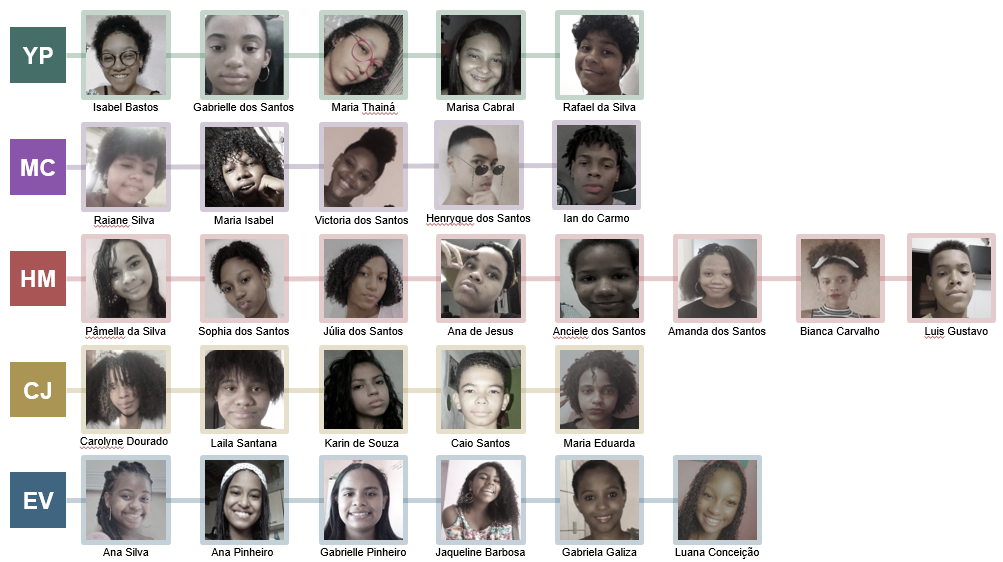
\includegraphics[width=13.93in]{images/image111} \caption{Equipe de estudantes bolsistas do projeto Ciência de Dados na Escola Pública}\label{fig:estudcdnaep}
\end{figure}

\hypertarget{equipe}{%
\section*{Equipe}\label{equipe}}
\addcontentsline{toc}{section}{Equipe}

Uma equipe multidisciplinar, composta por estudantes de graduação (5) e pós-graduação (7) e por professoras/es e profissionais que atuam em instituições de ensino superior se dividem em sete grupos de ação (ver Figura \ref{fig:profcdnaep}):

\begin{itemize}
\tightlist
\item
  Coordenação e Secretaria;
\item
  Ciência de Dados;
\item
  Inteligência Artificial;
\item
  Produção do Conhecimento Científico;
\item
  (re)Conhecendo Salvador;
\item
  Protagonismo;
\item
  Avaliação de Impactos do Projeto.
\end{itemize}

\begin{figure}
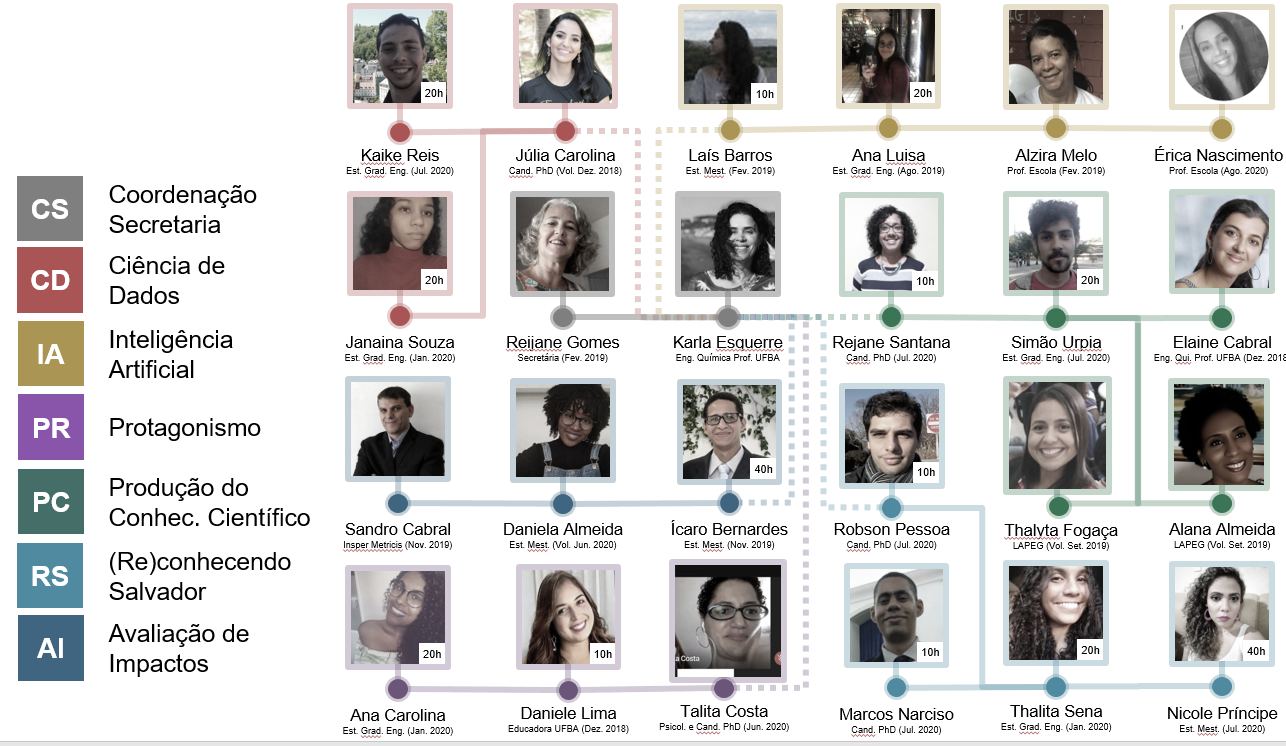
\includegraphics[width=17.86in]{images/image113} \caption{Equipe do projeto Ciência de Dados na Escola Pública}\label{fig:profcdnaep}
\end{figure}

\hypertarget{auxe7uxf5es-do-projeto}{%
\section*{Ações do Projeto}\label{auxe7uxf5es-do-projeto}}
\addcontentsline{toc}{section}{Ações do Projeto}

As atividades desenvolvidas durante o ano de 2020 podem ser agrupadas em cinco grandes ações, conforme descrito a seguir (seções 1-5). Juntamente com as demais seções, este relatório busca descrever de forma sucinta tais ações e seus resultados, assim como os desafios e dificuldades encontradas que exigiram o reajuste das atividades planejadas inicialmente.

\textbf{COLOCAR LISTA SUMARIO}

\hypertarget{construuxe7uxe3o-do-website-do-projeto}{%
\chapter{Construção do Website do Projeto}\label{construuxe7uxe3o-do-website-do-projeto}}

O \href{https://cienciadedadosep.wixsite.com/cdep/sobre}{website do Projeto} foi construído como ferramenta de compartilhamento de materiais para toda a comunidade escolar, professores, estudantes, coordenadores e gestores (ver Figura \ref{fig:pagcdnaep}). Visando facilitar o acesso ao site (de modo intuitivo) os conteúdos foram organizados e agrupados em: ``Início'', ``Sobre'', ``Café com Dados'', ``Professores'', ``Estudantes'' e ``Ferramentas'' . Na Figura \ref{fig:diagrpagcdnaep} é apresentado um mapa conceitual da página.
O site ``Ciência de Dados na Educação Pública'' foi desenvolvido em março, através do Wix, devido a facilidade apresentada pela plataforma na personalização e manipulação de conteúdo. Produzido através de um modelo de template oferecido pelo Wix, o design de interface e estrutura do site precisaram de algumas adaptações para adentrarem na identidade visual do projeto. Ademais estruturalmente, com o objetivo de ampliar a interação com os usuários, todas as páginas do site possuem um espaço para ``comentários''.
Os materiais presentes no website, foram designados de acordo com as demandas do projeto, dessa forma, a plataforma funcionava como um repositório de informações, sendo possível acessar apresentações, ferramentas, gravações e os mais diversos conteúdos apresentados pela equipe, com o intuito de facilitar as atividades assíncronas e síncronas.

\begin{figure}
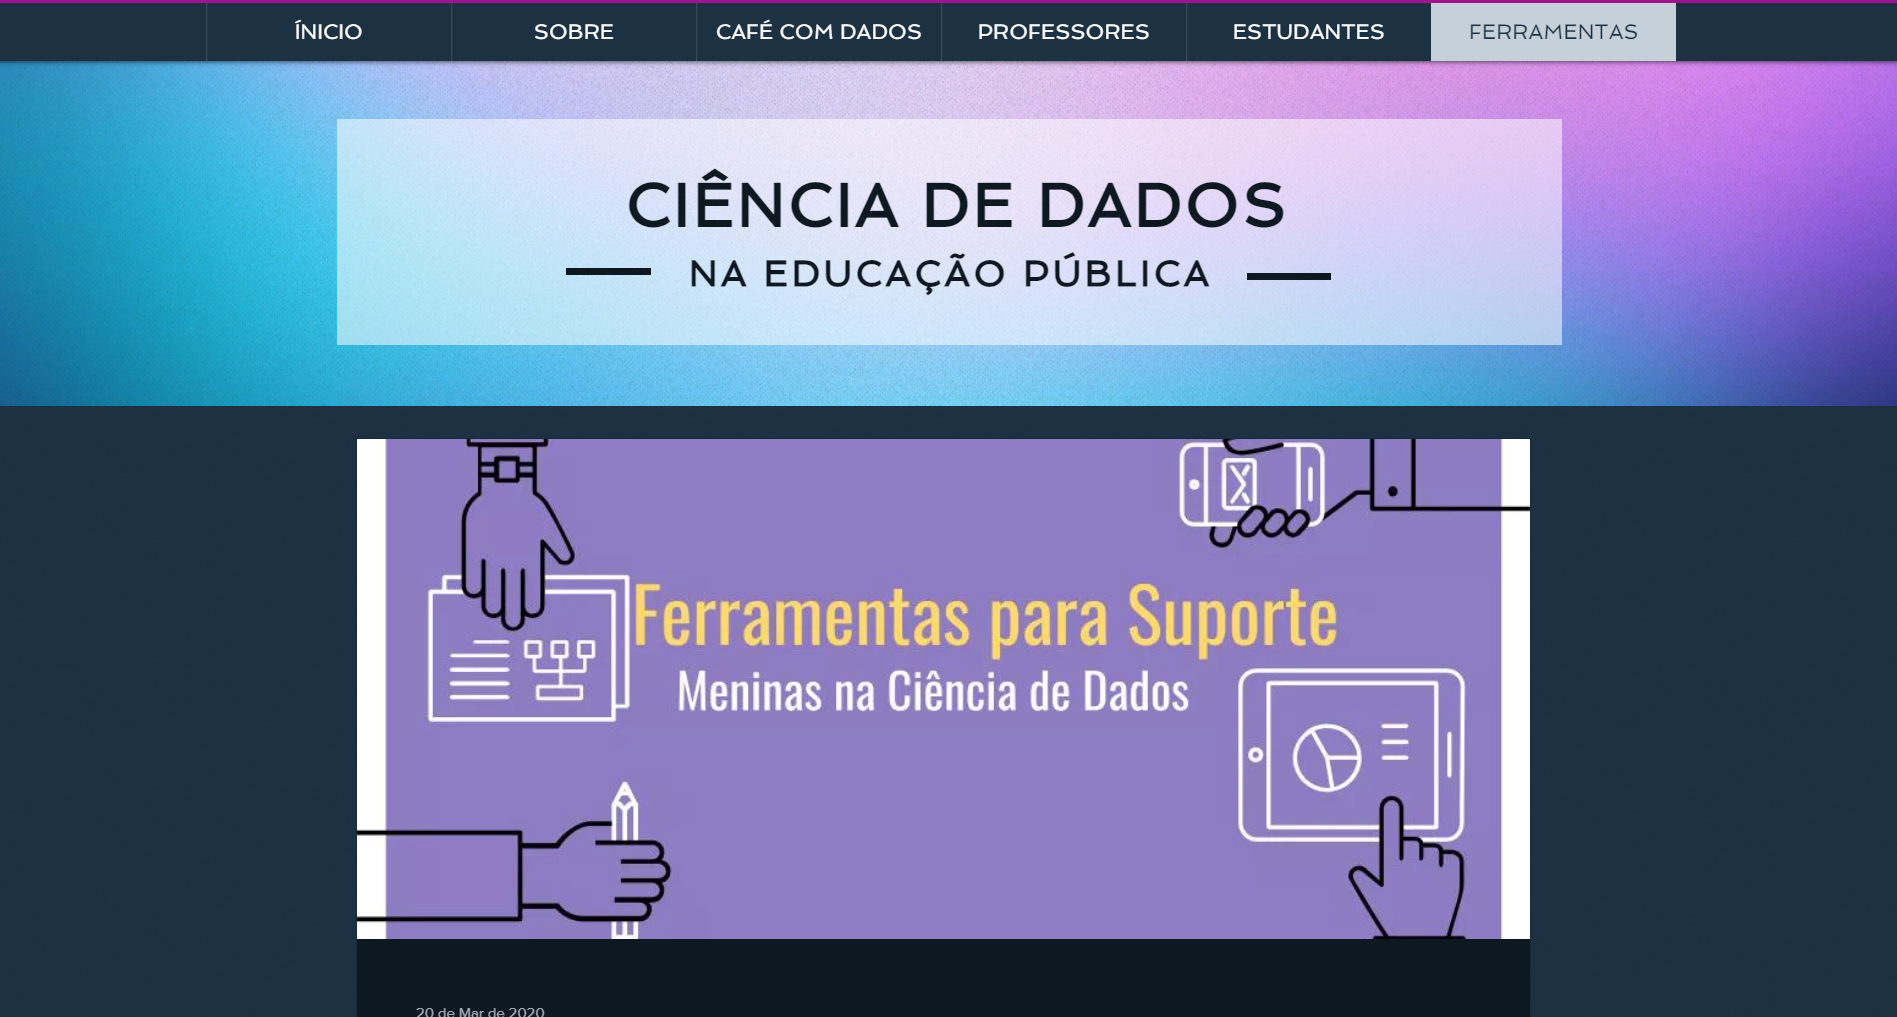
\includegraphics[width=26.35in]{images/image85} \caption{Página inicial do site do projeto Ciência de Dados na Escola Pública}\label{fig:pagcdnaep}
\end{figure}

\begin{figure}
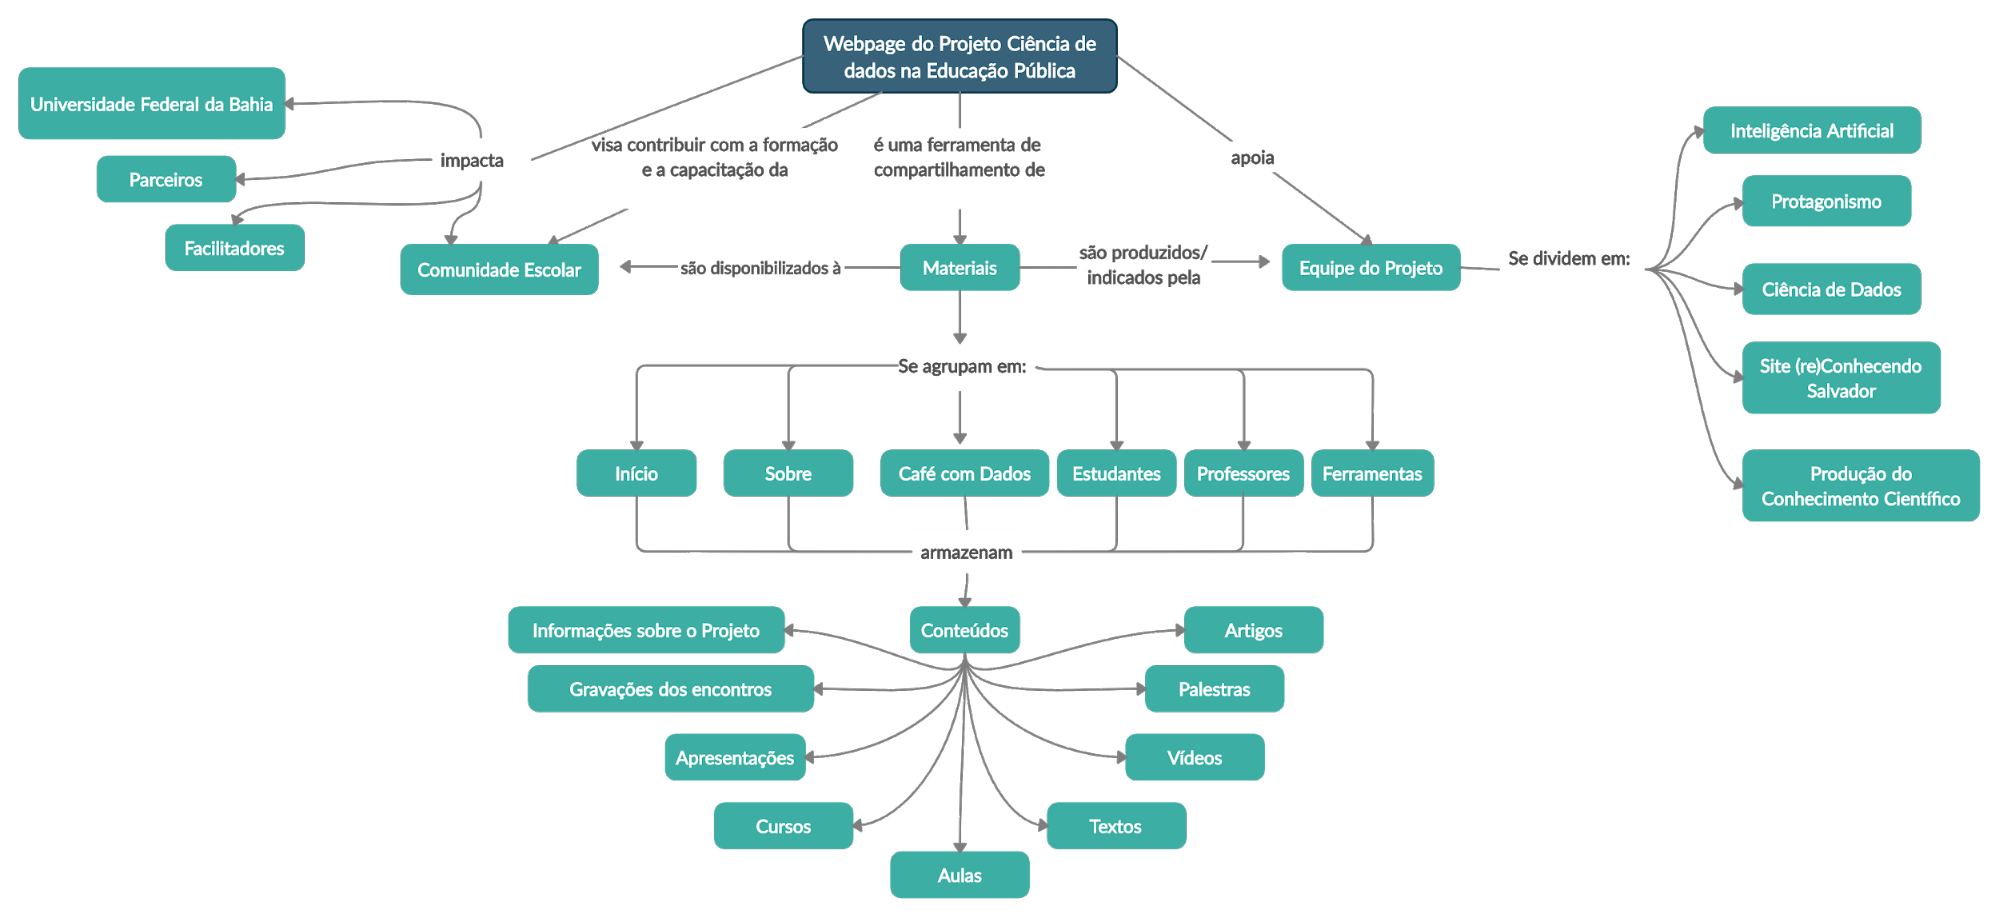
\includegraphics[width=27.76in]{images/image26} \caption{Página inicial do site do projeto Ciência de Dados na Escola Pública}\label{fig:diagrpagcdnaep}
\end{figure}

\hypertarget{puxe1ginas-do-website}{%
\section{Páginas do website}\label{puxe1ginas-do-website}}

\hypertarget{inuxedcio-e-sobre}{%
\subsection*{Início e Sobre}\label{inuxedcio-e-sobre}}
\addcontentsline{toc}{subsection}{Início e Sobre}

A página \href{https://cienciadedadosep.wixsite.com/cdep}{Início} foi projetada para ressaltar as informações de conhecimento imediato do público alvo. Desta maneira, a página contém a apresentação do projeto no Lemann Center Virtual Meeting - Stanford University, com o intuito de introduzir as ações, parcerias e resultados do projeto.
O menu \href{https://cienciadedadosep.wixsite.com/cdep/sobre}{Sobre}, descreve trajetória, proposta, idealizadores, equipe e parcerias do projeto Ciência de Dados na Educação Pública. Além de vídeos-posters sobre o projeto elaborados pelas bolsistas de graduação para a submissão no Congresso Virtual UFBA 2020.

\hypertarget{cafuxe9-com-dados}{%
\subsection*{Café com Dados}\label{cafuxe9-com-dados}}
\addcontentsline{toc}{subsection}{Café com Dados}

A página \href{https://cienciadedadosep.wixsite.com/cafecomdados}{Café com Dados} foi criada para oferecer auxílio aos professores que apresentavam algumas dificuldades para ingressar nos encontros como: pouco conhecimento do ambiente virtual dos encontros, falha na conexão com a internet, limitação de participantes na plataforma, dificuldade para visualizar a apresentação, falta de disponibilidade, dificuldade para escutar o palestrante.
Para enfrentar esses obstáculos, a Webpage dispõe dos temas, nome e atribuições dos palestrantes, slides, referências sugeridas e gravações de todas as palestras que ocorreram de 01/04/2020 à 07/10/2020 no Café com Dados.

\hypertarget{professores}{%
\subsection*{Professores}\label{professores}}
\addcontentsline{toc}{subsection}{Professores}

A seção \href{https://cienciadedadosep.wixsite.com/professores}{Professores}, foi idealizada para apresentar materiais de apoio para os docentes na área de Ciência de Dados, Inteligência Artificial, protagonismo feminino e programação. Dessa forma, o site é dividido em: ``Cursos'', ``Artigos'', ``Palestras'', ``Sites'', ``Vídeos'', ``Mulheres na Ciência'', ``Sistema de Dados'' e ``Programas''.
Alguns dos materiais sugeridos encontram-se na língua inglesa, deste modo, a equipe disponibilizou no site os tutoriais ``Como colocar legenda no vídeo do YouTube'' e ``Como traduzir uma página'' para auxiliar os professores.

\hypertarget{estudantes}{%
\subsection*{Estudantes}\label{estudantes}}
\addcontentsline{toc}{subsection}{Estudantes}

A webpage \href{https://cienciadedadosep.wixsite.com/estudantes}{estudantes} tem a finalidade de fornecer suporte e facilitar o acesso dos estudantes aos materiais manuseados pelo projeto. Inicialmente, a página continha apenas textos sobre as mulheres extraordinárias, cursos e palestras. Entretanto, no segundo semestre de 2020 o site passou a abranger os vídeos diários e os materiais utilizados nos encontros online, como apresentações, atividades e vídeos.

\hypertarget{ferramentas}{%
\subsection*{Ferramentas}\label{ferramentas}}
\addcontentsline{toc}{subsection}{Ferramentas}

A página \href{https://cienciadedadosep.wixsite.com/cdep/ferramentas}{ferramentas}, foi uma das primeiras seções a serem desenvolvidas no site, devido a urgência de instrumentos online para estimular os estudantes a manterem o interesse na escola. Dessa forma, o projeto apresentou, instruiu e disponibilizou na web page 10 ferramentas online de diversas áreas para os docentes das escolas parceiras.

\hypertarget{elaborauxe7uxe3o-de-4-e-books}{%
\chapter{\texorpdfstring{Elaboração de 4 \emph{e-books}}{Elaboração de 4 e-books}}\label{elaborauxe7uxe3o-de-4-e-books}}

O conteúdo dos E-books se subdivide em 4 temas: Ciências de dados, Inteligência artificial, Pensamento científico e Protagonismos. Os três primeiros são destinados aos estudantes e apresentam exemplos pautados na discussão sobre a cidade a partir do site (re)Conhecendo Salvador. As reflexões visam atingi-los, a fim de estimulá-los a se perceberem como protagonistas de mudanças da sociedade, capazes de promover ações nas escolas, em suas comunidades ou em outros contextos da cidade. Os capítulos dos e-books oferecem os objetivos da abordagem de cada assunto, o que se espera dos/as estudantes, sugestões de como abordar o tema em sala de aula, os principais vocábulos, sugestões de leituras, vídeos e páginas em redes sociais (Instagram, Facebook, Pinterest etc.).
O E-book sobre protagonismos social, racial e de gênero é o único volume que se destina especificamente aos professores e visa auxiliá-los na abordagem dos assuntos em sala de aula, dialogando com os conceitos de interseccionalidade (articulação entre raça, classe e gênero), autoconceito, autoestima e empoderamento. A diferenciação entre os protagonismos social, racial e de gênero é didática e visa apenas facilitar a discussão sobre os diferentes temas. Compreendemos que os sujeitos se caracterizam por distintos marcadores sociais e cotidianamente lidam com formas de discriminação sobrepostas. Por isso, necessitam se engajar em estratégias de enfrentamento de modo igualmente articulado.

\hypertarget{e-book-1.-ciuxeancia-de-dados-80-concluuxeddo}{%
\section{\texorpdfstring{\emph{e-book} 1. Ciência de Dados (\(80\%\) concluído)}{e-book 1. Ciência de Dados (80\textbackslash\% concluído)}}\label{e-book-1.-ciuxeancia-de-dados-80-concluuxeddo}}

Cap. 1 - Introduzindo a Ciência de Dados, Cap. 2 - Construindo uma Base de Dados, Cap. 3 - Visualizando Dados, Cap. 4 - Correlação e Causalidade; Cap. 5 - Estatística Inicial; Cap. 6 - Coletando Dados para Pesquisas; Cap. 7 - Distribuições, Probabilidade e Possibilidade; Cap. 8 - Entendendo e Avaliando suas Hipóteses; Cap. 9 - Classificação e Cap. 10 - Regressão.

\hypertarget{e-book-2.-inteliguxeancia-artificial-75-concluuxeddo}{%
\section{\texorpdfstring{\emph{e-book} 2. Inteligência Artificial (\(75\%\) concluído)}{e-book 2. Inteligência Artificial (75\textbackslash\% concluído)}}\label{e-book-2.-inteliguxeancia-artificial-75-concluuxeddo}}

Cap. 1. - Inteligência Artificial; Cap. 2 - Pensamento Computacional; Cap. 3 - Aprendizado de Máquina; Cap. 4 - Inteligência Artificial e Ciência de Dados; Cap. 5 - Eu como Protagonista de Mudanças na Sociedade; Cap. 5 - Planos de Aula e Materiais; Cap. 6 - Robótica e Programação Desplugada.

\hypertarget{e-book-3.-produuxe7uxe3o-do-conhecimento-cientuxedfico-50-concluuxeddo}{%
\section{\texorpdfstring{\emph{e-book} 3. Produção do Conhecimento Científico (\(50\%\) concluído)}{e-book 3. Produção do Conhecimento Científico (50\textbackslash\% concluído)}}\label{e-book-3.-produuxe7uxe3o-do-conhecimento-cientuxedfico-50-concluuxeddo}}

Cap. 1 - Origem da Ciência; Cap. 2 - Investigação Científica; Cap. 3 - Observações e Experimentos Científicos; Cap. 4 - Documento Científico; e a proposta de seis capítulos relacionados à investigação científica na prática (Quanta água tem na minha fruta? O ovo dobrável; Batata com sal, os outros capítulos estão em construção), os experimentos citados se relacionam com conhecimentos das ciências da natureza (química, física e biologia), e tem como objetivo servir de ferramenta para o professor explorar junto com os estudantes o fenômeno da evaporação, conhecimentos sobre a composição química de diferentes frutas, pH, além de possibilitar descobertas relacionadas ao seu cotidiano.

\hypertarget{e-book-4.-protagonismo-social-racial-e-de-guxeanero}{%
\section{\texorpdfstring{\emph{e-book} 4. Protagonismo Social, Racial e de Gênero}{e-book 4. Protagonismo Social, Racial e de Gênero}}\label{e-book-4.-protagonismo-social-racial-e-de-guxeanero}}

\hypertarget{protagonismo-social-proposta-em-andamento}{%
\subsection{Protagonismo Social (proposta em andamento)}\label{protagonismo-social-proposta-em-andamento}}

Cap. 1 - O Grito dos(as) Excluídos(as); Cap. 2 - Direitos e Deveres da Criança e do Adolescente. O demais capítulos estão em processo de definição.

\hypertarget{protagonismo-racial-80-concluuxeddo}{%
\subsection{\texorpdfstring{Protagonismo Racial (\(80\%\) concluído)}{Protagonismo Racial (80\textbackslash\% concluído)}}\label{protagonismo-racial-80-concluuxeddo}}

Cap. 1 - Blackface, Representatividade negra e Preconceito racial na mídia; Cap. 2 - Colorismo e branquitude; Cap. 3 - Interseccionalidade: raça, gênero e classe; Cap. 4 - Literatura negra; Cap. 5 - Mito da Democracia Racial; Cap. 6 - Necropolítica; Cap. 7 - Racismo no ambiente escolar; Cap. 8 - Racismo e Intolerância Religiosa; Cap. 9 - Políticas de Ações Afirmativas e o Dia Internacional de Luta contra a discriminação racial; Cap. 10 - Tokenismo, segregação e discriminação algorítmica na Inteligência Artificial.

\hypertarget{protagonismo-de-guxeanero-0-concluuxeddo}{%
\subsection{\texorpdfstring{Protagonismo de Gênero (\(0\%\) concluído)}{Protagonismo de Gênero (0\textbackslash\% concluído)}}\label{protagonismo-de-guxeanero-0-concluuxeddo}}

Cap. 1 - A trajetória da construção do conceito (de mulher para gênero); Cap. 2- Sexo e sexualidade; Cap. 3 - Identidade de gênero (homens e mulheres cisgênero e transgênero); Cap. 4 - Orientação sexual (heterossexualidade, homossexualidade e bissexualidade); Cap. 5 - Sexo biológico e expressão de gênero (masculina, feminina e não-binária); Cap. 6- Diversidade sexual e cidadania; Cap. 7 - Movimentos sociais LGBTQI+ e a luta/conquista de direitos; Cap. 8 - Discursos hegemônicos e narrativas sobre homens e mulheres na sociedade brasileira; atribuição de papéis e expectativas sociais; Cap. 9 - Violência de gênero e violência contra a mulher; Cap. 10 - Diversidade sexual na escola e a Atenção à criança e ao adolescente vítima de discriminação por orientação sexual e identidade de gênero; Cap. 11- Representatividade feminina nas ciências; Cap. 12- Protagonismo de gênero e Lei de Diretrizes e Bases (LDB); Cap. 13 - Protagonismo de gênero, Ciência de Dados e Inteligência Artificial (IA).
Na Figura \ref{fig:ebookcd} é apresentado o mapa conceitual do E-book 1 - Ciência de Dados e a Figura \ref{fig:ebookprotag} exemplifica a apresentação visual do conteúdo do Capítulo 2 deste mesmo e-book.

\begin{figure}
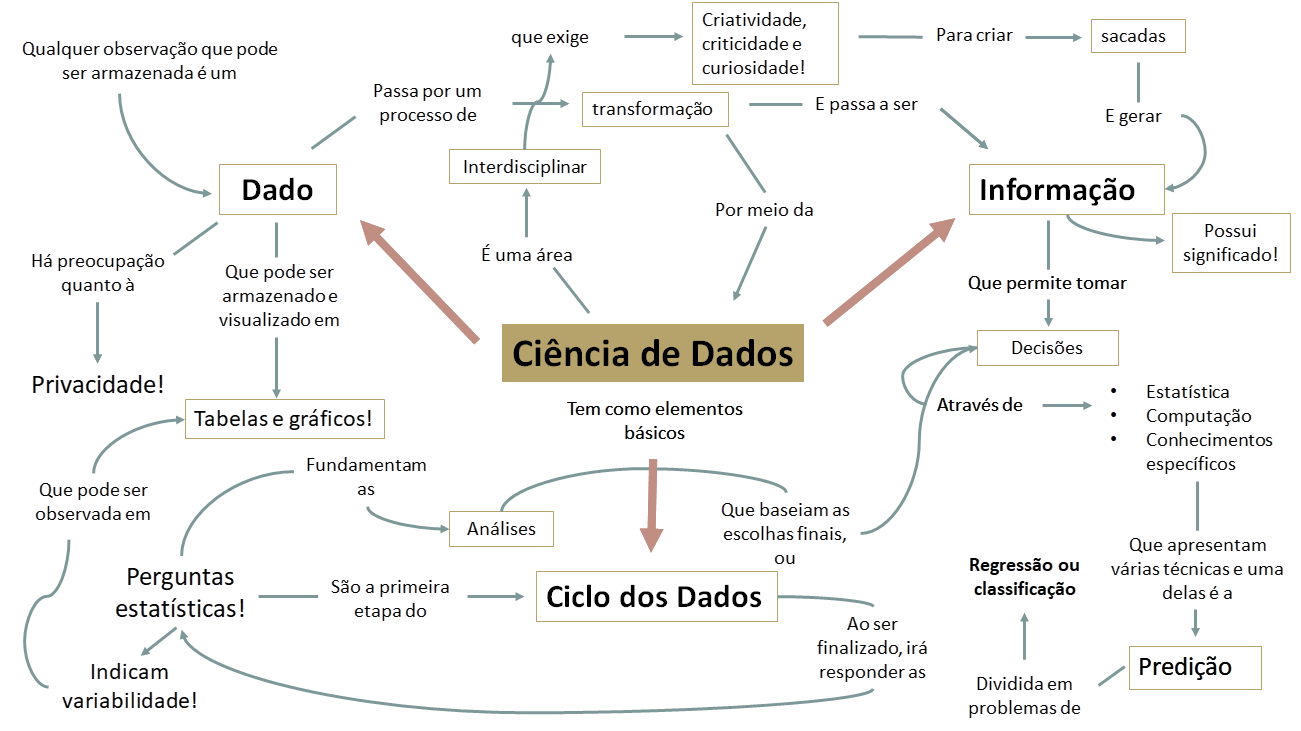
\includegraphics[width=18.07in]{images/image115} \caption{Mapa conceitual do E-book 1 – Ciência de Dados.}\label{fig:ebookcd}
\end{figure}

\begin{figure}
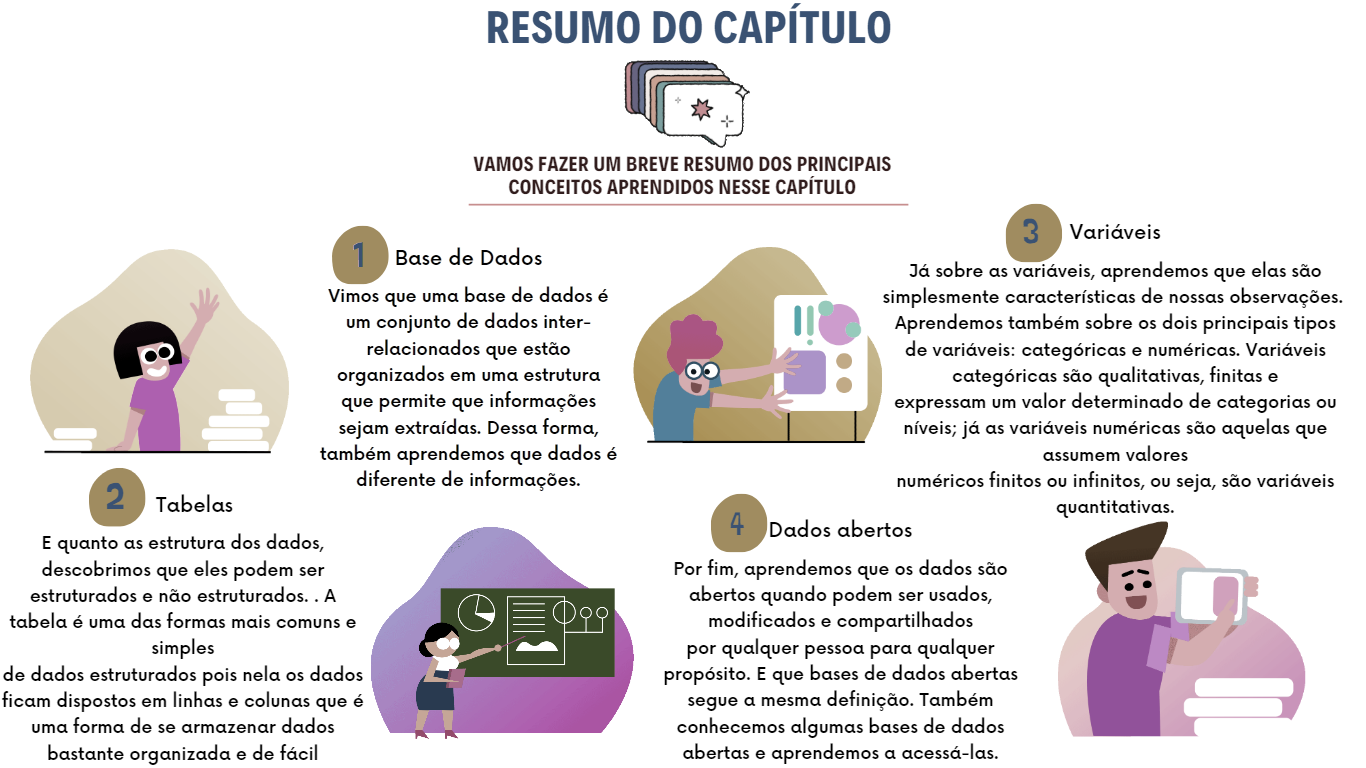
\includegraphics[width=18.97in]{images/image116} \caption{Imagem apresentada no Capítulo 2 do E-book de Ciência de Dados.}\label{fig:ebookprotag}
\end{figure}

\hypertarget{elaborauxe7uxe3o-de-site-com-estatuxedsticas-histuxf3ricas-da-cidade-de-salvador}{%
\chapter{Elaboração de site com estatísticas históricas da cidade de Salvador}\label{elaborauxe7uxe3o-de-site-com-estatuxedsticas-histuxf3ricas-da-cidade-de-salvador}}

A construção do site (re)Conhecendo Salvador requer a realização de cinco etapas: (1) Briefing; (2) Conteúdo; (3) Design; (4) Desenvolvimento e (5) Publicação. A etapa (1) está concluída. Dados e estatísticas de Salvador são explorados individualmente ou conectando os seguintes grandes temas: Educação, Turismo, Segurança, População e Famílias, Ciência e Tecnologia, Lazer e Desporto, Saúde, Transporte, Meio Ambiente e Justiça. Um mapa conceitual deste site é apresentado na Figura \ref{fig:recossa}. A partir das experiências trazidas pelos estudantes são exploradas e sua visão da cidade e sociedade ampliada com a exploração gráfica de dados e estatísticas. Tais habilidades tentam fortalecê-los ao se perceberem como agentes de mudanças da sociedade.

\begin{figure}
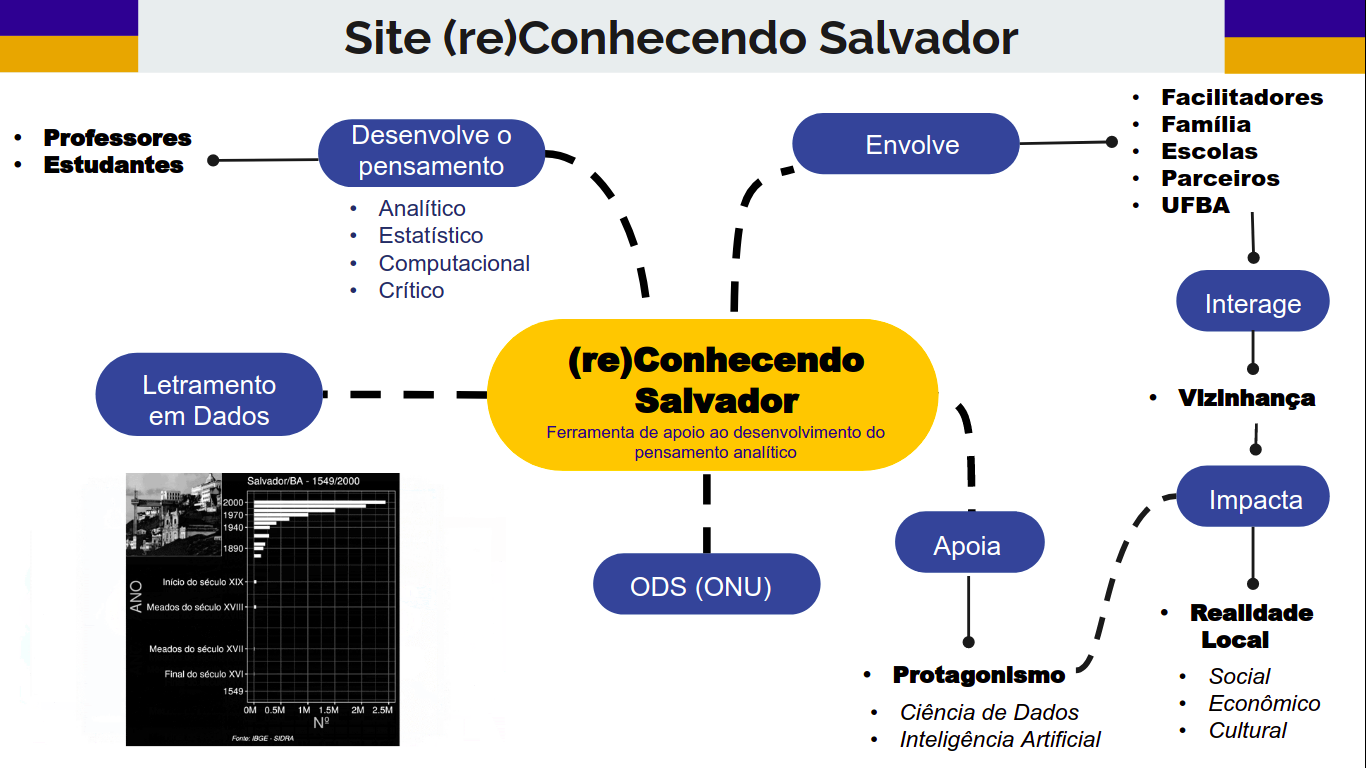
\includegraphics[width=18.97in]{images/mapaconceitualressa} \caption{Desenho esquemático do site (re)Conhecendo Salvador.}\label{fig:recossa}
\end{figure}

Um processo de licitação está em andamento para a contratação de empresa para realizar as etapas (2) e (3). A produção do conteúdo (etapa 5) está em andamento através da definição das perguntas, do levantamento (\emph{webscraping}) dos dados e estatísticas para responder a estas perguntas e da definição de gráficos que sejam visualmente atrativos e que permitam a visualização de tendências e padrões (quando existirem). No \textbf{Apêndice 12.1} são listadas perguntas trazidas pelos estudantes e levantadas pela equipe cujos dados e estatísticas já foram inferidos.

\hypertarget{construuxe7uxe3o-e-explorauxe7uxe3o-do-site-reconhecendo-salvador}{%
\section{Construção e exploração do site (re)Conhecendo Salvador}\label{construuxe7uxe3o-e-explorauxe7uxe3o-do-site-reconhecendo-salvador}}

\hypertarget{etapas-de-desenvolvimento-do-site-reconhecendo-salvador}{%
\section{Etapas de desenvolvimento do site (re)Conhecendo Salvador}\label{etapas-de-desenvolvimento-do-site-reconhecendo-salvador}}

A ideia do desenvolvimento do site (re)Conhecendo Salvador surgiu ainda no projeto \emph{Meninas na Ciência de Dados}. Ela foi inspirada no projeto \href{https://www.pordatakids.pt/Inicio}{PorData Kids}, desenvolvido pela Fundação Francisco Manuel dos Santos, que explora estatísticas de Portugal a partir de questionamentos levantados em diversas áreas como educação, saúde, meio ambiente, transportes entre outros.
O (re)Conhecendo Salvador servirá como ferramenta de apoio ao desenvolvimento do pensamento analítico a ser utilizado pelos professores e estudantes do projeto, pois irá retratar a realidade da cidade de Salvador através de questionamentos cujas respostas são fundamentadas através de dados. Para isso, algumas perguntas foram levantadas com as estudantes durante ações do próprio projeto, formando um banco de perguntas.
Para dar início ao desenvolvimento, em abril de 2020, ocorreu a primeira reunião entre as equipes do projeto e da empresa de desenvolvimento InfoJr., para fazer o primeiro briefing com o levantamento de requisitos do site e proposta orçamentária. Posteriormente, já com a equipe do site em ação, novas reuniões foram realizadas para definir o escopo do site. Portanto, as etapas de mapa do site e definição de itens estão concluídas.
O levantamento dos dados para o desenvolvimento do banco de dados responsável por abastecer o site começou em Agosto. Esta etapa ainda está em andamento em decorrência da dificuldade de encontrar dados abertos e que respondam ao nosso banco de perguntas. Para agilizar o desenvolvimento do banco de dados, algumas perguntas estão sendo reformuladas de acordo com os dados já levantados.
A Figura \ref{fig:steprecossa} apresenta as etapas de desenvolvimento do site. Em relação ao relatório de setembro, tivemos um avanço significativo a partir das entregas da logomarca e identidade visual do (re)Conhecendo Salvador. O design de interface, entretanto, é uma etapa que continua em andamento porque apenas uma tela foi desenvolvida, a tela inicial, porém, a partir dela, e da identidade visual feita pela Alinhavo Jr.~será continuado o trabalho de design de interface das páginas seguintes de forma interna.

\begin{figure}
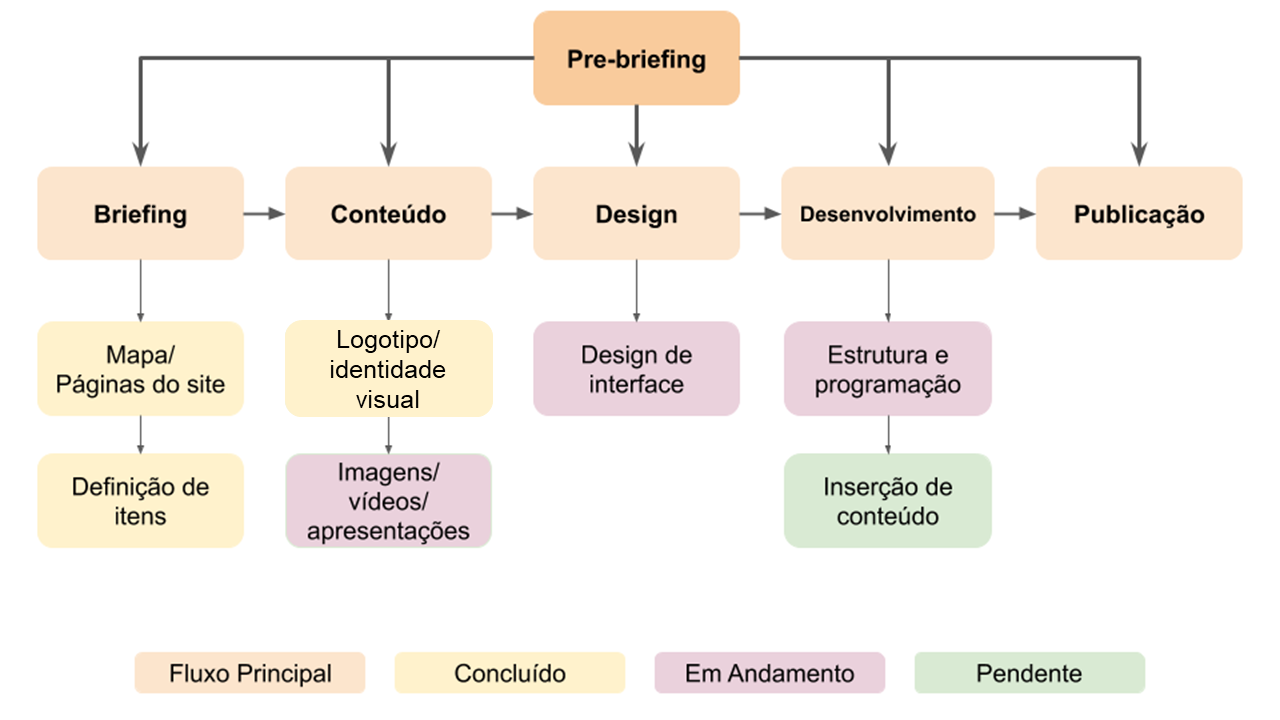
\includegraphics[width=17.78in]{images/image108} \caption{Fluxo do processo de desenvolvimento do site (re)Conhecendo Salvador.}\label{fig:steprecossa}
\end{figure}

\hypertarget{relato-da-contratauxe7uxe3o-da-empresa-de-design-gruxe1fico-alinhavo-jr.-e-entrega-da-identidade-visual-e-puxe1gina-principal-do-site-reconhecendo-salvador}{%
\section{Relato da contratação da empresa de design gráfico Alinhavo Jr.~e entrega da identidade visual e página principal do site (re)Conhecendo Salvador}\label{relato-da-contratauxe7uxe3o-da-empresa-de-design-gruxe1fico-alinhavo-jr.-e-entrega-da-identidade-visual-e-puxe1gina-principal-do-site-reconhecendo-salvador}}

No início do mês de setembro, foi enviado o Termo de Referência para
contratação de empresa especializada na prestação de serviços de design gráfico à FAPEX. Entretanto, dentro do prazo estipulado no edital, não houve submissões de empresas candidatas, fazendo-se necessária a prorrogação do prazo por três vezes. Por se tratar de um processo licitatório, era preciso ter, pelo menos, 3 propostas de empresas candidatas para realizar a contratação, entretanto, só houve uma empresa interessada e, assim, foi solicitado ao setor jurídico da FAPEX a aprovação desta proposta para dar início ao desenvolvimento da identidade visual e da interface do site (re)Conhecendo Salvador. Todo esse processo consumiu, aproximadamente, 50 dias do projeto, sendo a contratação da empresa efetivada no início do mês de novembro.
De acordo com o edital, a empresa contratada deveria desenvolver e entregar, em um prazo de 8 semanas ininterruptas, os seguintes produtos:

\begin{itemize}
\tightlist
\item
  A identidade visual do (re)Conhecendo Salvador;
\item
  A página principal do site contendo no mínimo:

  \begin{enumerate}
  \def\labelenumi{\roman{enumi}.}
  \tightlist
  \item
    Logomarca do site (Re)Conhecendo Salvador;
  \item
    Menu superior;
  \item
    Ilustração com temática de (Re)Conhecendo Salvador;
  \item
    Menu inferior.
  \end{enumerate}
\end{itemize}

A partir do aceite da FAPEX para a contratação da única empresa candidata ao edital, foram realizadas 5 reuniões da equipe do site com a empresa Alinhavo Jr.. A primeira reunião foi solicitada pela equipe do projeto para comunicar a aprovação da proposta pela FAPEX (29/10/2020). As demais reuniões foram solicitadas pela Alinhavo Jr.~para apresentar a equipe responsável por desenvolver a identidade visual e a interface do site, além do cronograma de entregas, dando início ao processo de imersão da empresa (19/11/2020), que foi continuado no na semana seguinte (26/11/2020), a partir de uma demanda da equipe do site de incluir estudantes do projeto Ciência de Dados na Educação Pública.
Posteriormente, ocorreram outras reuniões para realizar entregas parciais (11/01/2021 e 20/01/2021). Por ser um processo iterativo e incremental, o cronograma de entrega precisou ser reajustado, dadas as necessidades de mudança no processo de construção dos produtos solicitados pela própria equipe do site (re)Conhecendo Salvador. Detalhes dos encontros estão descritos a seguir.

\hypertarget{etapas-de-desenvolvimento-da-homepage-do-site-reconhecendo-salvador}{%
\section{Etapas de desenvolvimento da homepage do site (re)Conhecendo Salvador}\label{etapas-de-desenvolvimento-da-homepage-do-site-reconhecendo-salvador}}

O desenvolvimento da tela inicial do site (re)conhecendo Salvador foi
realizado de forma incremental entre as partes. Quando a equipe recebeu
a confirmação da contratação da empresa Alinhavo Jr.~pela FAPEX,
marcou-se uma reunião inicial (29/10/2020) com as duas equipes, dando
início ao alinhamento de expectativas e processo de desenvolvimento da
identidade visual e da interface do site.
Durante a reunião, novamente, foi apresentada a proposta do projeto, ressaltada a sua relevância e o seu impacto social. O site (re)Conhecendo Salvador, que foi inspirado em um site de Portugal (Pordata Kids), tem como público estudantes de escolas públicas do ensino fundamental 2, e deveria trazer um ``mapa'' da cidade como ilustração principal, sem perder o aspecto funcional da cidade, retratando suas particularidades, que incluem os contrastes sociais, sua historicidade, porém sem parecer um marketing turístico. A Alinhavo Jr.~aproveitou a oportunidade para solicitar que a equipe do site apresentasse referências para que eles pudessem começar o processo de criação dos produtos. Então, foram enviados por e-mail as principais referências de sites para a concepção do (re)Conhecendo Salvador (\href{https://www.pordatakids.pt/}{Pordatakids}; \href{https://educa.ibge.gov.br/}{Educa IBGE} e \href{https://www.youcubed.org/pt-br/}{YouCubed}), além de relatórios e apresentações sobre os projetos ``Meninas na Ciência de Dados'' e ``Ciência de Dados na Educação Pública'' e suas respectivas logomarcas.

Após a assinatura do contrato em 06 de novembro de 2020, a Alinhavo Jr.~solicitou uma nova reunião para apresentar oficialmente a equipe responsável por desenvolver o projeto de identidade visual e interface do site. A partir dessa nova reunião, a equipe do site passou a contar com a colaboração da Professora Drª. Roseline Vanessa Santos Oliveira, líder do Laboratório de Investigações de Núcleos Habitados (LIN-A), da Universidade Federal de Alagoas (UFAL). A Prof.~Roseline trouxe observações bastante pertinentes e relevantes sobre os aspectos históricos e urbanísticos da cidade de Salvador, como a percepção dos sentidos como a audição (os sons da cidade de Salvador e a sua musicalidade), o olfato e o paladar (o cheiro característico da cidade proveniente de sua cultura e culinária), além dos aspectos artístico presentes no mais diversos lugares da cidade, remontando, muitas vezes, não apenas suas origens quanto influências sofridas da fundação e desenvolvimento da cidade de Salvador. Durante essa reunião, a equipe do site solicitou que a Alinhavo Jr.~incluísse no processo de criação a participação dos estudantes atuais do projeto o que gerou a necessidade de uma reunião exclusiva com esses estudantes e uma extensão do prazo em 10 dias. Ainda nesta reunião, ficou acordado que a equipe deveria responder a um questionário elaborado pela própria empresa Jr.~assim como também seria elaborado um questionário específico para os estudantes, para captação de dados. Após essa reunião, a Alinhavo Jr.~disponibilizou os links dos formulários para serem respondidos pela equipe, e pelos estudantes. Os links foram publicados no canal geral do Slack do projeto e no grupo de WhatsApp dos estudantes, junto com uma mensagem de solicitação para o preenchimento dos formulários por todos.
Após o preenchimentos dos formulários, os estudantes foram convidados a participarem de um encontro extra (26/11/2020) sobre o desenvolvimento do site (re)Conhecendo Salvador no dia . Em função do horário da reunião divergir dos horários de atividades combinados previamente com os estudantes e seus familiares, houve pouca adesão - aproximadamente 10/25 estudantes participaram do novo encontro com a empresa Jr.~e poucos se manifestaram no chat ou por áudio. Para equilibrar a baixa interatividade dos estudantes nessa reunião e, ainda, captar mais informações deles, foi sugerido pela equipe do site que eles fizessem um esboço ou desenho sobre Salvador ou como eles imaginavam que seria o site de acordo com a proposta do projeto. A Alinhavo Jr.também elaborou um novo questionário que foi enviado aos estudantes para mais coleta de informações.
A primeira entrega parcial aconteceu no dia 11 de janeiro de 2020 na presença de toda a equipe desenvolvedora da identidade visual da Alinhavo Jr.~juntamente com a equipe do site, a Prof.~Roseline e pesquisadores do ``Ciência de Dados na Educação Pública''. Na entrega parcial foi apresentada a concepção da logomarca do site, a justificativa pela escolha das cores e como a logomarca se relaciona com o projeto. Em seguida, foi apresentada a interface da tela inicial do site, de forma detalhada, desde a apresentação dos menus, da ilustração, das seções de apresentação do site, projeto e grupo de pesquisa, apresentação da equipe, e contatos. Ao final, a equipe do site, junto com as professoras Karla Esquerre e Roseline apontaram aspectos que precisavam ser ajustados para atingir o objetivo do projeto. A ilustração principal não trazia os aspectos funcionais da cidade e nem respondiam aos temas do menu superior (como educação, saúde, emprego, ciência e tecnologia), estava muito focada nos aspectos históricos e turísticos de Salvador. Também foram solicitadas alterações menores como na cor dos botões, nas cores do logo, para ficarem mais vivas, mudança nos títulos das abas da seção ``Sobre o projeto'' de ``História'' para ``Percurso'' e ``Atividades'' para ``Dinâmicas'', mudança na seção ``nossa equipe'' por um único elemento fotográfico, além do desenho de fundo da página, e por fim, uma pequena alteração no rodapé. Ficou acordado entre as partes, o envio de uma nova versão em 48 horas.
Na nova versão, havia um esboço da ilustração inicial bastante modificada e mais adequada aos objetivos do site, mas ainda precisava de algum refinamento. Por e-mail foram solicitadas as seguintes alterações:

\textbf{Tela inicial}

\begin{itemize}
\tightlist
\item
  Substituir a ilustração do prédio da reitoria do IFBA pelo prédio do Barbalho, onde realmente estão concentrados os cursos técnicos e de graduação, pois consideramos ser uma estrutura mais marcante, além de ser a sede (IFBA Barbalho).
\item
  Colocar as comunidades de Salvador representadas em morros/encostas, uma vez que Salvador é uma cidade de geografia bastante acidentada e marcada pelos seus relevos. Pensar que essa representação poderia ficar ao fundo do hospital e se parecer com a comunidade da Gamboa (Gamboa);
\item
  Incluir a ilustração de uma baiana junto das pessoas do menu de população, sem grandes destaques, apenas como pessoa que faz parte da população de Salvador;
\item
  Manter a ilustração do Dique do Tororó com os orixás. Pensamos que, com a modificação das casas das comunidades para atrás do hospital, esse espaço poderia ser ocupado pelo TJ e, assim, o Dique poderia retornar ao espaço onde estava na primeira sugestão de ilustração, embaixo da passarela;
\item
  Adicionar na ilustração a frase ``Andar com fé eu vou que a fé não costuma faiá'' de Gilberto Gil como elemento sonoro que representa Salvador;
\item
  Adicionar na tela inicial o slogan do projeto ``Conhecer e experimentar para compreender e transformar.'';
\item
  Alterar o menu superior para um menu horizontal na versão desktop;
\item
  Aumentar a fonte das informações de contato.
\end{itemize}

\textbf{Sobre o projeto}

\begin{itemize}
\tightlist
\item
  Trocar a ilustração ao lado direito do canto superior pelo Pelourinho com a igreja azul, Nossa Senhora do Rosário dos Pretos (pode ser a ilustração da tela inicial da primeira proposta);
\item
  Substituir o rapaz negro no canto inferior esquerdo por uma mulher acompanhada de uma criança (mãe e filha);
\item
  Aumentar a fonte do texto dentro dos boxes de percurso, dinâmica e Gamma.
\end{itemize}

\textbf{Equipe}

\begin{itemize}
\tightlist
\item
  Substituir gráficos de fundo por uma ilustração da entrada da politécnica, pois representa o lugar onde a equipe está localizada (Politécnica) e a própria UFBA, que não apareceu em outros lugares do site.
\end{itemize}

A entrega dos produtos foi realizada no dia 28 de Janeiro de 2021 através do compartilhamento dos arquivos em nuvem. Abaixo, serão apresentadas a logomarca e a tela inicial do site.
A logomarca é o elemento de identidade visual mais representativo. Assim, a logomarca do projeto foi desenvolvida para conversar entre a proposta do projeto Ciência de Dados na Educação Pública e do grupo de pesquisa GAMMA. A proposta que foi apresentada pela Alinhavo Jr.~e aceita pela equipe está apresentada na Figura \ref{fig:logorecossa}.

\begin{figure}

\includegraphics[width=27.76in]{images/image100} \caption{ Logomarca oficial do site (re)Conhecendo Salvador.}\label{fig:logorecossa}
\end{figure}

A logomarca traz elementos que representam o sol e as pessoas, assim como o céu de Salvador. O movimento das ondas do mar está representado através de parábolas, que se abraçam, trazendo a sensação do afeto que é tão importante para o projeto. Os ``dedos'' também fazem alusão à representação do gráfico de barras, representando a ciência de dados e a estatística.
A interface da página inicial do site (re)Conhecendo Salvador aprovada pela equipe está apresentada nas figuras \ref{fig:ilustrecossa}, \ref{fig:sobrerecossa}, \ref{fig:equiperecossa} e \ref{fig:contatorecossa} (ilustração, sobre o projeto, equipe e contato respectivamente).

\begin{figure}
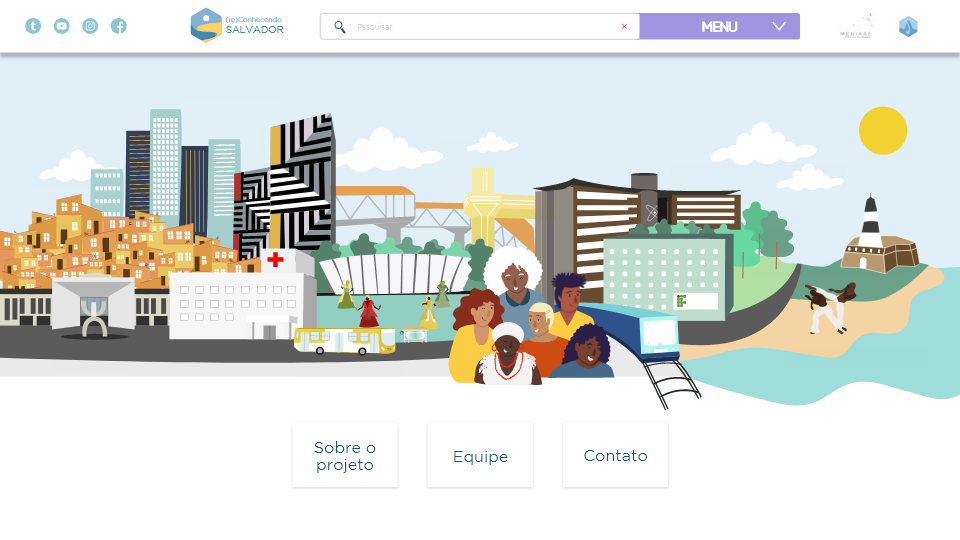
\includegraphics[width=13.33in]{images/image29} \caption{Apresentação e ilustração/menu do site (re)Conhecendo Salvador}\label{fig:ilustrecossa}
\end{figure}

\begin{figure}
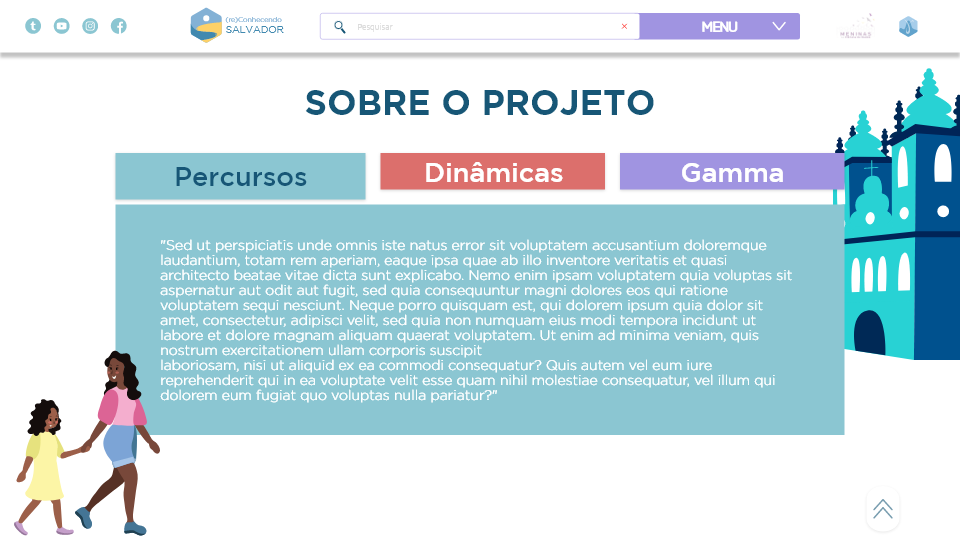
\includegraphics[width=13.33in]{images/image7} \caption{Seção “Sobre o Projeto”.}\label{fig:sobrerecossa}
\end{figure}

\begin{figure}
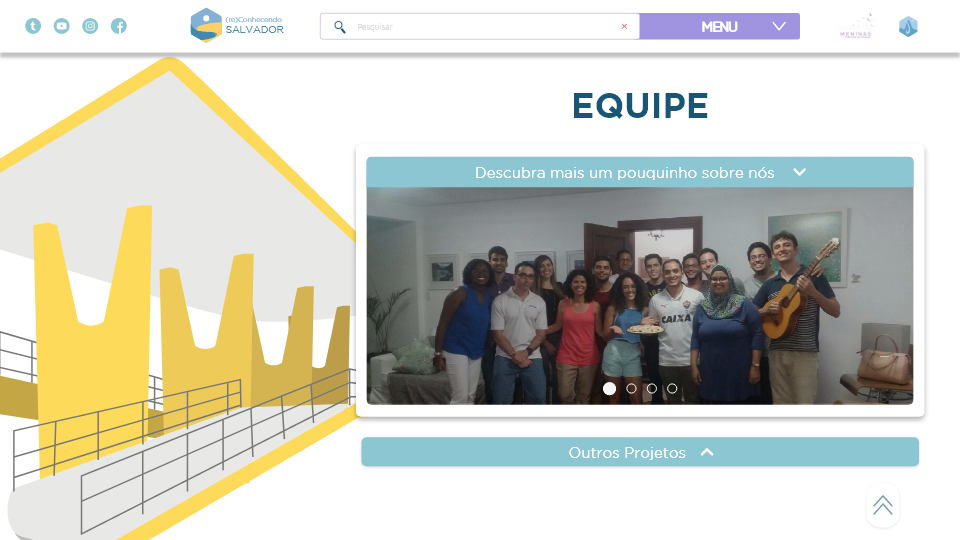
\includegraphics[width=13.33in]{images/image23} \caption{Seção “Equipe”.}\label{fig:equiperecossa}
\end{figure}

\begin{figure}
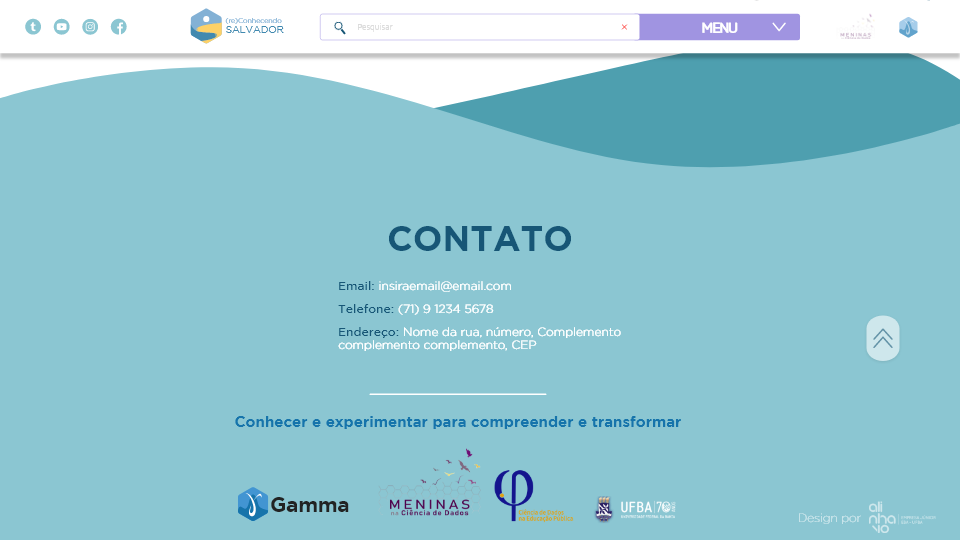
\includegraphics[width=13.33in]{images/image90} \caption{Seção “Contato”.}\label{fig:contatorecossa}
\end{figure}

Durante o período de licitação da empresa de desenvolvimento da \emph{homepage}, a equipe dedicou-se ao desenvolvimento de uma versão beta do site que é detalhado nas seções a seguir.

Durante o período de licitação da empresa de desenvolvimento da \emph{homepage}, a equipe dedicou-se ao desenvolvimento de uma versão beta do site que é detalhado nas seções a seguir.

\hypertarget{desenvolvimento-do-site-na-versuxe3o-beta-teste-com-muxf3dulos-gruxe1ficos}{%
\section{Desenvolvimento do site na versão beta (teste) com módulos gráficos}\label{desenvolvimento-do-site-na-versuxe3o-beta-teste-com-muxf3dulos-gruxe1ficos}}

Em função das dificuldades para a contratação de empresas para o
desenvolvimento do site (re)Conhecendo Salvador, a equipe resolveu
desenvolver uma versão beta (de teste) internamente utilizando o
gerenciador de conteúdo (CMS) Wordpress, que é uma plataforma
gratuita, open source bastante robusta e confiável, utilizada em sites de grandes empresas como a Walt Disney, Globo (G1), Sony Music e Toyota. Para isso, inicialmente foi feita uma capacitação online e gratuita através da plataforma Mirago.
A capacitação em Wordpress durou, aproximadamente, duas semanas, e ocorreu em paralelo às demais atividades do projeto. Para desenvolver o site (re)Conhecendo Salvador utilizando o Wordpress foi necessário instalar no computador servidores web e de banco de dados (Apache e MySQL), através do MAMP 4.2.0, que é um pacote de servidores que prepara o ambiente localhost para receber o gerenciador de conteúdos. Somente após a instalação dessa infraestrutura é possível instalar o Wordpress na máquina. Vale salientar que a versão utilizada no desenvolvimento deste site foi o Wordpress.org, e por isso foi necessário preparar o ambiente da máquina para recebê-lo. Ele foi escolhido em detrimento da versão Wordpress.com por ser mais customizável e atender melhor aos requisitos do site.
A próxima etapa de desenvolvimento do (re)Conhecendo Salvador versão beta foi a pesquisa e escolha do tema a ser utilizado no wordpress. O tema corresponde à uma estrutura básica de telas que pode ser instalada no wordpress.org e customizada de acordo com as necessidades da proposta do site. Foi feita uma pesquisa de temas para descobrir o melhor custo benefício para desempenho e funcionalidades do site. Dentro das opções gratuitas, foi escolhido o tema Neve pois apresenta uma estrutura mais robusta e flexível, permitindo customizações das telas nos mais diversos aspectos. Após a instalação do CMS e da escolha do tema, ainda foi necessário fazer a instalação do plugin Elementor, dentro do Wordpress, na versão gratuita, para aprimorar as possibilidades de construção de layouts das telas.
A diagramação das telas seguiu o fluxo de telas do site Pordata Kids: tela inicial \textgreater{} tela de submenus dos temas \textgreater{} painel de perguntas \textgreater{} dashboards com gráficos. A logomarca, os elementos do menu principal e os botões foram todos criados utilizando dos recursos gratuitos oferecidos na plataforma de design online Canva (Figura \ref{fig:logotrecossa}, \ref{fig:botaotrecossa}, \ref{fig:voltartrecossa} e \ref{fig:botaointtrecossa})

\begin{figure}
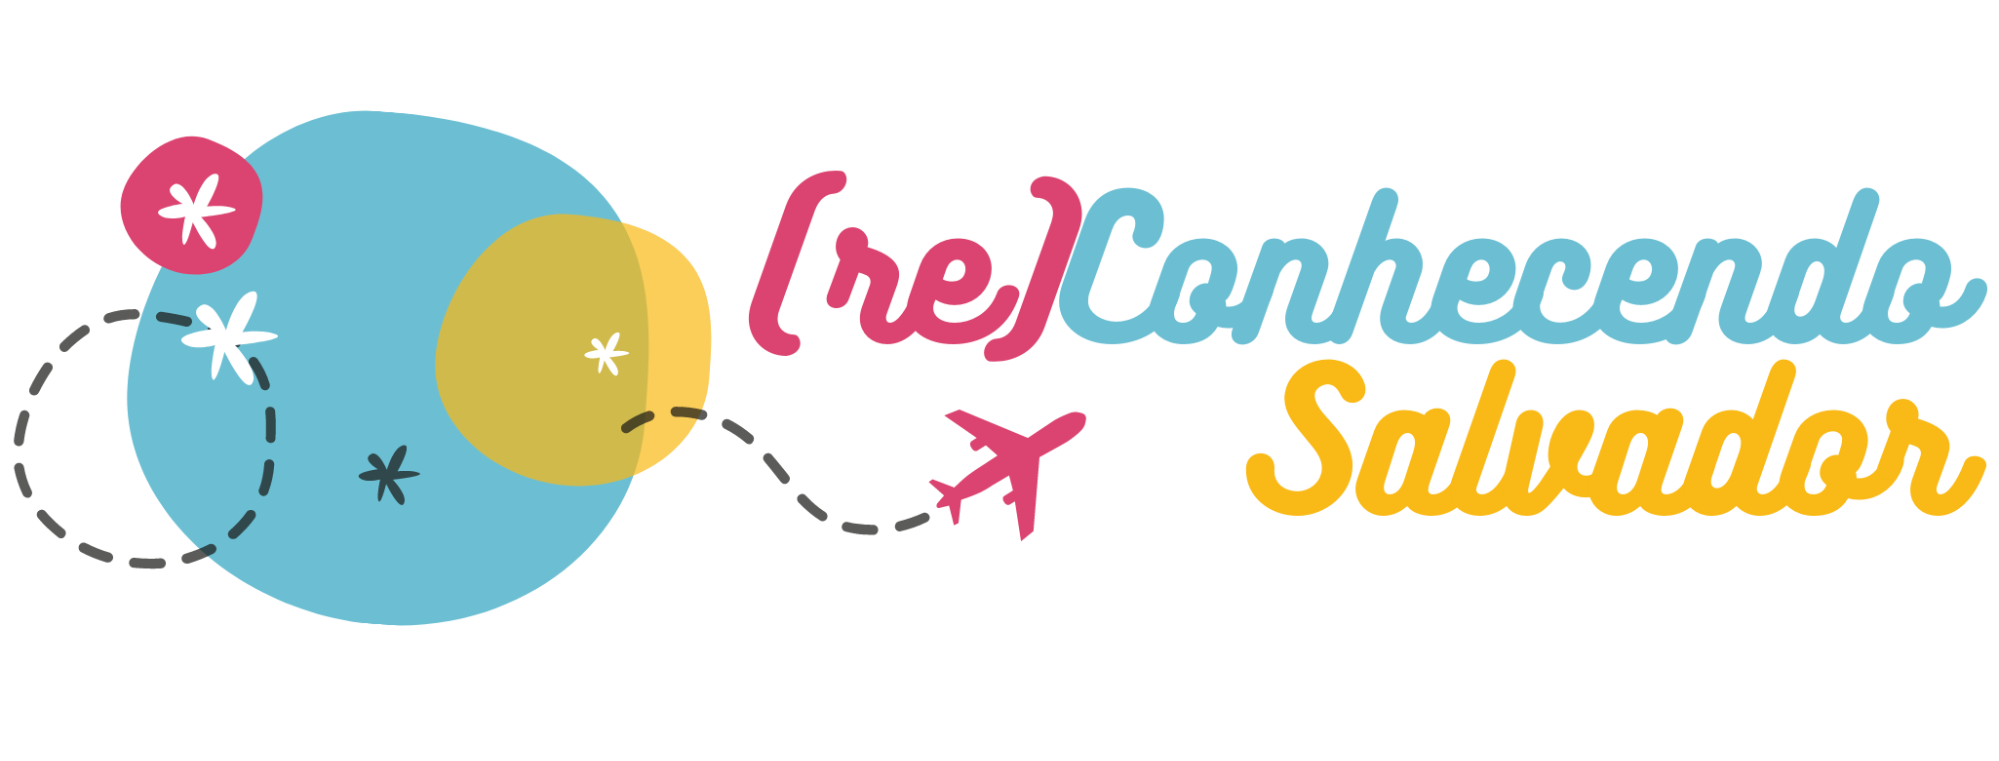
\includegraphics[width=0.5\linewidth]{images/image11} \caption{Logomarca da versão teste.}\label{fig:logotrecossa}
\end{figure}

\begin{figure}
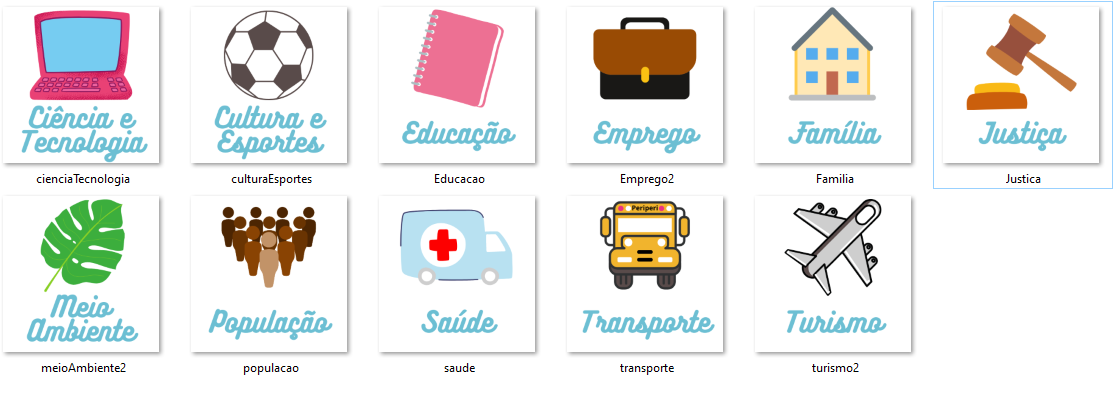
\includegraphics[width=1.5\linewidth]{images/image80} \caption{Botões do menu principal}\label{fig:botaotrecossa}
\end{figure}

\begin{figure}

\includegraphics[width=0.5\linewidth]{images/image69} \caption{Botão de rodapé.}\label{fig:voltartrecossa}
\end{figure}

\begin{figure}
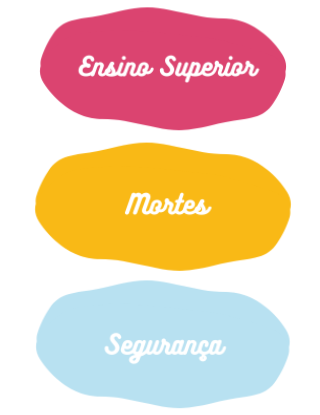
\includegraphics[width=0.5\linewidth]{images/image27} \caption{Botões dos painéis dos subtemas educação, população e segurança, de cima para baixo, respectivamente.}\label{fig:botaointtrecossa}
\end{figure}

Depois de iniciar o desenvolvimento na máquina local, optamos por transferir a versão a um servidor online e gratuito para que outros membros da equipe pudessem visualizar e até mesmo modificar a estrutura do que estava proposto. Após algumas pesquisas, o servidor escolhido foi o \href{https://www.awardspace.com/}{Awardspace}. Esse servidor oferece instalador automático do WordPress, o que facilitou bastante a migração da versão desenvolvida no computador local para o servidor online, hospedagem sem anúncios, além de ter espaço em disco igual a 1GB, largura de banda de 5GB, e banco de dados MySQL. Para fazer a migração, foi necessário instalar no wordpress da máquina o plugin All-in-One, nativo no Wordpress do Awardspace. Entretanto, após fazer a migração para o servidor online, a equipe achou melhor continuar o desenvolvimento em localhost e utilizar o servidor online apenas para apresentar e compartilhar as mudanças e evoluções nas versões.

Os dados relacionados aos temas são apresentados em dashboars, embutidos nas páginas de respostas das perguntas, desenvolvidos em R, conforme descrito na seção ``Descrição do layout dos dashboards''.

A seguir, serão apresentadas as telas da versão teste do (re)Conhecendo Salvador de acordo com o fluxo de navegação:

\begin{itemize}
\tightlist
\item
  Tela inicial (Figura \ref{fig:teleinicialtrecossa})
\item
  Painel do submenu dos Temas (Figura \ref{fig:painelsubtrecossa})
\item
  Painel de Perguntas (Figura \ref{fig:paineldisptrecossa} )
\item
  Dashboard com a apresentação dos dados em gráficos (Figura \ref{fig:dashtrecossa})
\end{itemize}

\begin{figure}
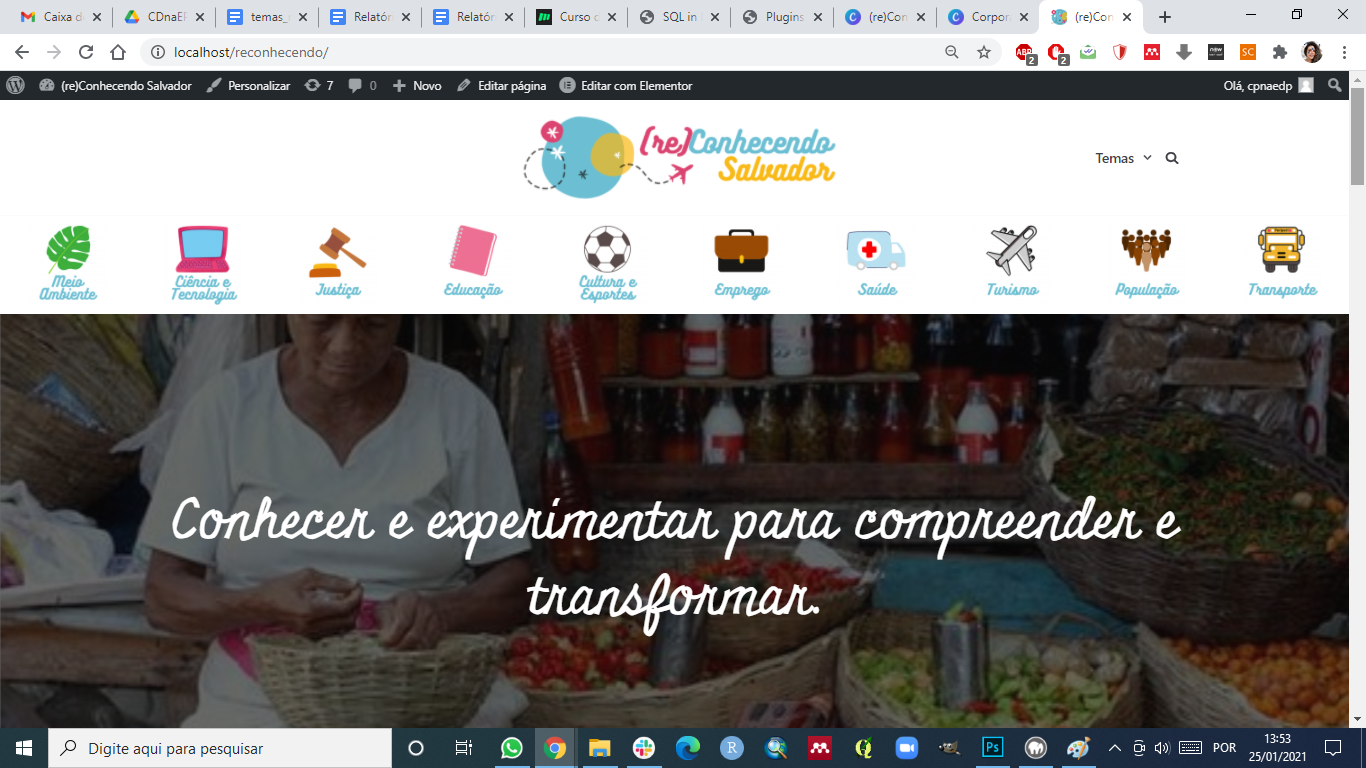
\includegraphics[width=1\linewidth]{images/image61} \caption{Tela inicial/ Página Principal.}\label{fig:teleinicialtrecossa}
\end{figure}

\begin{figure}
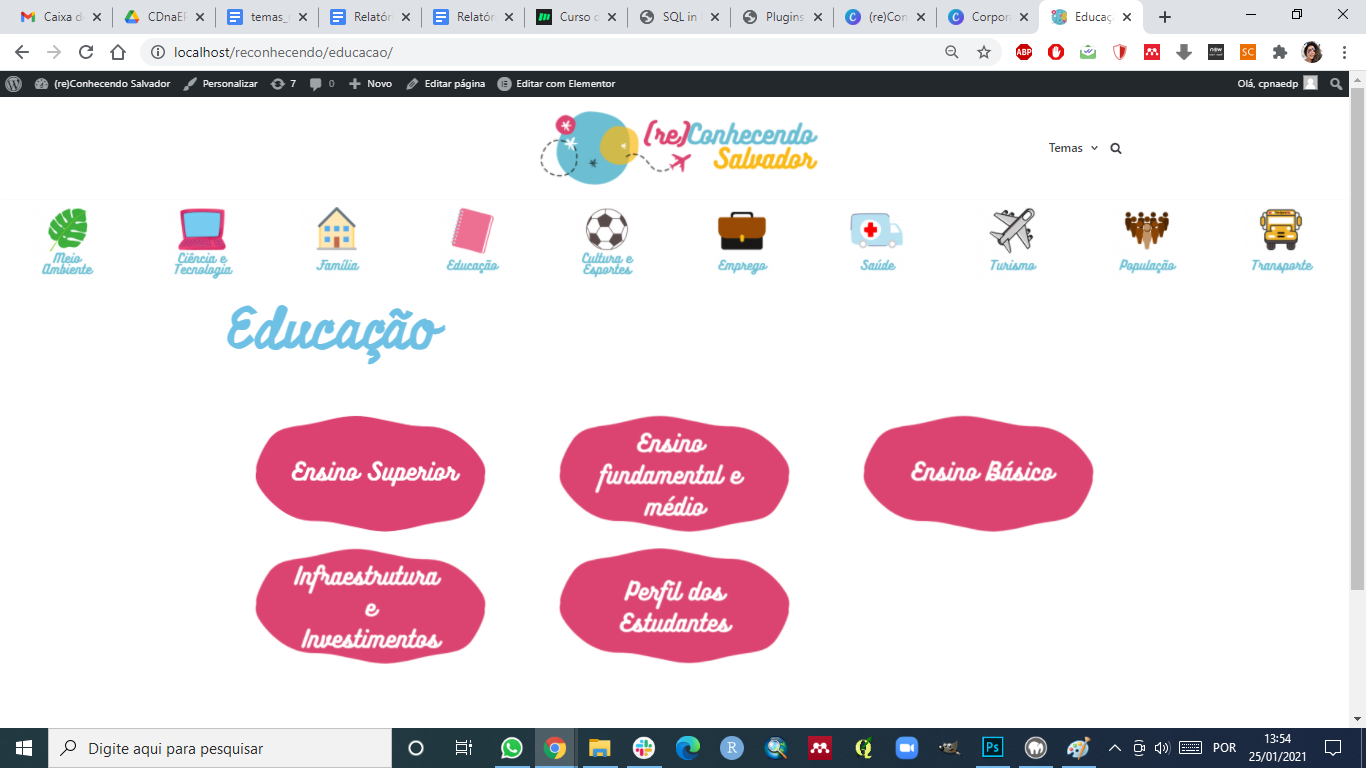
\includegraphics[width=1\linewidth]{images/image74} \caption{Painel do submenu do tema.}\label{fig:painelsubtrecossa}
\end{figure}

\begin{figure}
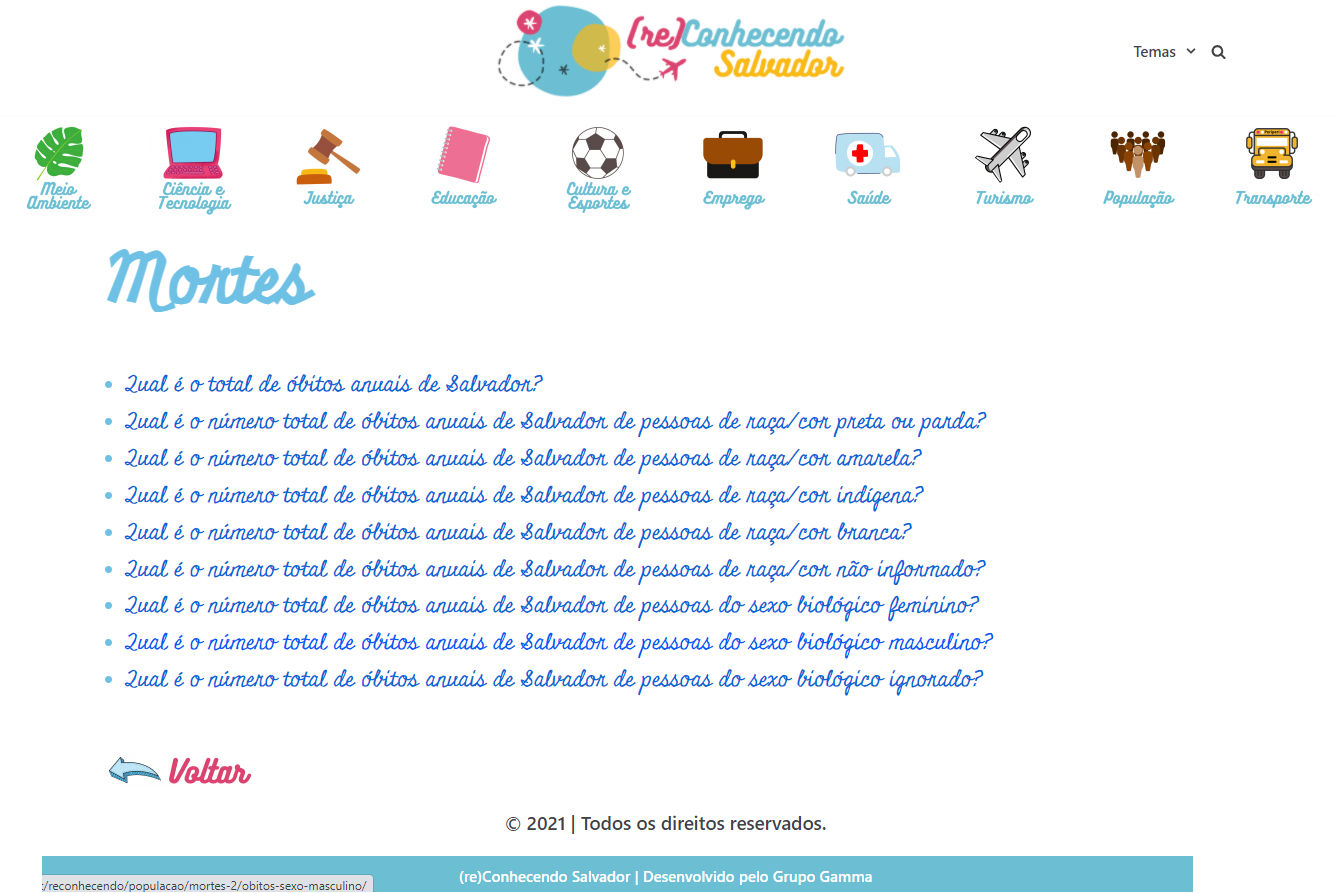
\includegraphics[width=1\linewidth]{images/image92} \caption{Painel de perguntas disparadoras.}\label{fig:paineldisptrecossa}
\end{figure}

\begin{figure}
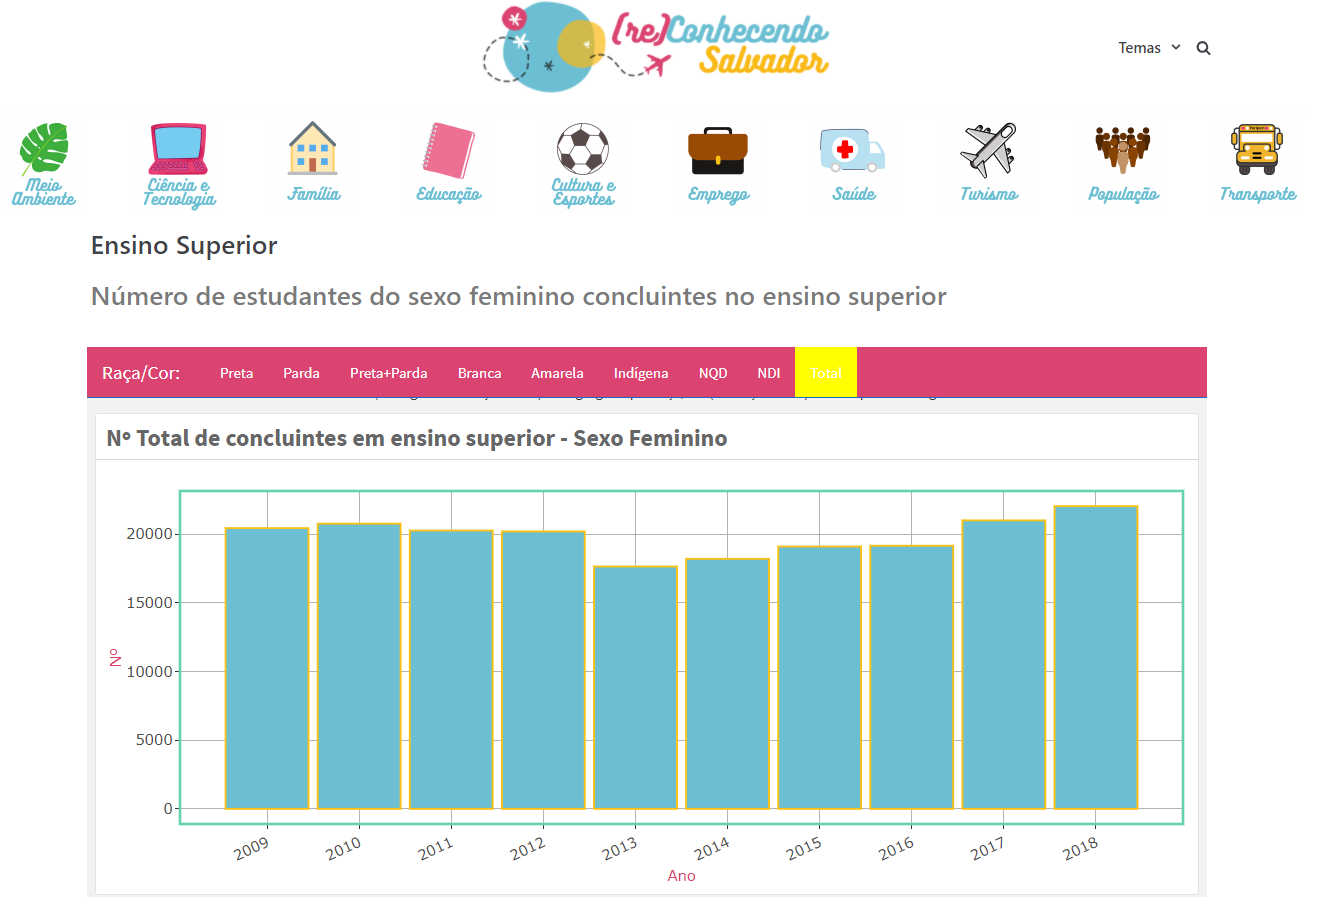
\includegraphics[width=1\linewidth]{images/image77} \caption{Painel de perguntas disparadoras.}\label{fig:dashtrecossa}
\end{figure}

\hypertarget{levantamento-dos-dados-e-informauxe7uxf5es}{%
\section{Levantamento dos Dados e Informações}\label{levantamento-dos-dados-e-informauxe7uxf5es}}

A representação gráfica de dados públicos é uma prática muito comum na área de Data Science. Entretanto, o processo de representação de informações está sujeito inicialmente à qualidade da pesquisa, ou seja, ele é tão mais relevante para sua interpretação quanto mais precisa é a informação. Mas não apenas estes elementos são importantes, a seleção adequada das formas gráficas, cores e aspectos dinâmicos podem interferir nesse desempenho do uso da informação. A ciência de dados formalmente tem as seguintes etapas: coleta, limpeza, análise exploratória, desenvolvimento e implementação do modelo. Em quase todas as etapas, a visualização de dados tem um papel fundamental como ferramenta na construção da informação. Assim, o elemento da visualização de dados pode ser utilizado como forma de introdução do estudante de escola pública na área de dados da sua cidade e em paralelo como mecanismo de familiarização com ciência de dados.
O processo de construção de informações é razoavelmente longo e pode surgir de diferentes objetivos e enfrenta limitações para realização das pesquisas de campo, bem como o registro e gestão desta informação. Estes aspectos são a priori essenciais para determinar a qualidade da informação obtida, bem como a capacidade de ajudar em análises estatísticas. O acesso aos diferentes níveis de informação, a forma como é disponibilizada também limita a capacidade de análise. O IBGE por exemplo possibilita por meio de um cadastro e treinamento para grupos pré-avaliados, a forma mais elementar da suas pesquisas num sistema chamado Banco Multidimensional de Estatísticas (BME) que contém os microdados das pesquisas e os respectivos metadados. Recentemente, a Escola Nacional de Administração Pública (Enap) vinculada ao Ministério da Economia (ME), produziu o livro Guia brasileiro de análise de dados: armadilhas \& soluções, neste documento são demonstrados de forma não tão introdutória os principais desafios em diferentes bancos de dados públicos. Ainda na apresentação do livro os autores são bem enfáticos em apontar que mesmo pesquisadores experientes, frente a um banco de dados novos, podem cometer equívocos na interpretação das informações. Alcançar o público dos estudantes não é uma tentativa isolada, é muito comum no mundo científico, especialmente em instituições de pesquisa e museus a prática de desenvolvimento de materiais didáticos, paradidáticos, jogos e ações para difusão do conhecimento científico para estudantes. Instituições como a Fiocruz, CEMADEN, Butantan, INPE e etc, promovem estes tipos de ações com recortes específicos das respectivas áreas. Quando tratamos de uma cidade, do meio urbano, da geografia temos IBGE que dispõem de ações como Educa IBGE dedicado a crianças e adolescentes. A maioria desses materiais e sistemas em certa medida estão distantes da realidade estudantil e fica necessário o papel da escola realizar esta aproximação de vivência do estudante e as informações e materiais disponíveis por essas instituições. O desenvolvimento do site por meio da visualização de dados da cidade de Salvador cumpre de forma mais adequada este papel.\\
Nas escolas públicas há uma grande variedade de experiências dos estudantes e por outro lado há uma mudança da forma de apresentação das informações que cada vez mais ampliam em qualidade e quantidade devido aos avanços tecnológicos. Devido às pressões geradas para a tomada de decisões baseada em informações de instituições ligadas ao governo federal, estadual e prefeituras municipais há uma necessidade clara da preparação do estudante para este mundo da informação e tecnologia. Letrar-se neste universo complexo e de disputas de narrativas exige o conhecimento empírico do mundo da informação como posta e a sua plena mudança. O caminho estabelecido pelo mundo das ferramentas livres, bem como a legislação de dados abertos abre possibilidades sem precedentes. A inclusão dos estudantes neste universo é uma ação de acesso a linguagem com que o mundo realiza as suas disputas, exclusões e recorte de oportunidades.\\
Desde o procedimento de pesquisa para coleta de dados de interesse públicos, o objetivo que definiu a necessidade dessa informação e a política de disponibilização de informações configuram um cenário bastante sensível às interpretações. Dado o contexto de letramento em dados deve-se considerar que devemos potencializar a aproximação dos estudantes aos dados por meio das suas próprias experiências. Neste sítio em desenvolvimento desejamos a priori que o estudante tenha uma imersão em séries históricas de dados sobre a evolução da população, crimes, eventos esportivos, educação etc. Todos esses temas relacionados à cidade de Salvador. Naturalmente, em alguma medida o estudante é capaz de interpretar informações de outras cidades e quiçá outros países, mas a hipótese essencial do projeto é que mergulhado na sua realidade o estudante vai além da interpretação ingênua. Ele torna-se capaz de argumentar sobre sua realidade. Passa dessa maneira a ser agente de proposição confrontado com pares com conhecimento e vivências similares. Essa dinâmica foi experimentada em certa medida em encontros realizados com 30 estudantes de 5 escolas públicas de Salvador.
O levantamento das informações que auxiliam nas respostas às perguntas disparadoras dos estudantes são realizadas com os seguintes pilares:

\begin{itemize}
\tightlist
\item
  Os dados tem que ser abertos;
\item
  Disponibilizados em sites de governos e organizações não governamentais, preferencialmente que sejam tabulados e rastreáveis;\\
\item
  Aqueles que promovam debates interessantes aos estudantes e professores.
\end{itemize}

Respeitado tais critérios, também é necessário algum desenvolvimento para a qualificação do dado ou informação. Dada a complexidade dos bancos de dados disponibilizados ao nível de microdados (desagregados de forma individualizada) é preciso um processo de compatibilização entre os diferentes anos e ao final é preciso uma etapa de verificação da informação. Após esta etapa, é da natureza deste trabalho a verificação visual da informação como forma de avaliação da riqueza da informação como meio de um processo educativo. Assim, essas etapas metodológicas são cumpridas por meio de recursos de programação como linguagens python, R, Bash e recursos de captura de informações de pdf.\\
Na lista abaixo descrevemos alguns avanços dos bancos de dados ligados aos temas e questões apresentados pelos estudantes e professores participantes de atividades do projeto Meninas nas Ciências de Dados - 2019:

\hypertarget{dados-de-populauxe7uxe3o}{%
\subsection{Dados de População}\label{dados-de-populauxe7uxe3o}}

Informações sobre a população brasileira em geral são disponibilizadas de forma desagregada ao nível dos municípios pelos produtos gerados pelo Instituto Brasileiro de Geografia e Estatística (IBGE), de forma organizada tais informações são encontradas no site (\url{https://cidades.ibge.gov.br/}). Particularmente no livro Geografia de Salvador de Andrade, Adriano Bittencourt (2009) é apresentado levantamento de informações sobre a dimensão da população de Salvador em épocas que precedem a existência do IBGE, partindo de meados do século XVI até o ano 2000 (Censo demográfico de 2000). O interesse dos estudantes em dados não é limitado à evolução do tamanho absoluto da população, mas suas divisões etárias, de gênero e raça que foram exploradas para composição do banco de dados do projeto. O subtema da população é muito central no debate sobre Salvador e o coloca num dos maiores desafios de desigualdade social encontrado nas metrópoles brasileiras. Portanto, o uso dos dados do Censo Demográfico são fundamentais na composição dos bancos de dados. Mas a imersão do estudante na sua localidade pode ser melhor explorada quando a informação é desagregada ao nível do seu bairro, como disponibilizado pela Casa Civil da prefeitura de Salvador (\url{http://casacivil.salvador.ba.gov.br}). O Programa das Nações Unidas para o Desenvolvimento (PNUD) construiu um resumo de informações sobre Salvador que está digitalmente apresentado na página (\url{http://www.atlasbrasil.org.br/perfil/municipio/292740\#sec-demografia}), na qual os dados estão desagregados por sexo biológico e raça. Embora sejam dados simples, eles remetem aos eixos transversais de temas críticos nas dimensões de desigualdade social.

\hypertarget{dados-de-educauxe7uxe3o}{%
\subsection{Dados de Educação}\label{dados-de-educauxe7uxe3o}}

Os dados de educação do ensino básico, fundamental e superior estão disponíveis como dados abertos no site do Instituto Nacional de Estudos e Pesquisas Anísio Teixeira - INEP. Os dados de educação utilizados são oriundos do Censo Escolar dos anos de 2009-2019, Censo do Ensino Superior de 2009-2019, dados georreferenciados das escolas públicas de Salvador (site: \url{http://educacao.salvador.ba.gov.br/educacao-em-numeros/}), arquivos vetoriais georreferenciados dos bairros e das prefeituras bairro de Salvador foram obtidos a partir de cooperação da Secretaria da Fazenda. Algumas informações foram obtidas do Atlas Brasil - PNUD Programa das Nações Unidas para o Desenvolvimento. Parte das informações construídas de tais bancos foram verificadas por meio do site: \url{https://www.qedu.org.br/}. Informações ligadas ao Ensino Superior são verificadas pela comparação entre relatórios institucionais de universidades como os gerados pela Pró-Reitoria de Planejamento e Orçamento da Universidade Federal da Bahia (Proplan/UFBA) e a agregação de microdados disponibilizados pelo Instituto Nacional de Educação Anísio Teixeira. Informações sobre a estrutura das escolas, no formato de dashboard, foram disponibilizadas pelo pesquisador em Dados Abertos Fernando Barbalho.

\hypertarget{dados-de-turismo}{%
\subsection{Dados de Turismo}\label{dados-de-turismo}}

Dados de Turismo foram coletados a partir de informações disponibilizadas a partir de relatórios das Secretaria de Turismo do Estado da Bahia -- SETUR, Superintendência de Investimentos em Zonas Turísticas -- SUINVEST, Diretoria de Planejamento Turístico -- DPT. Detalhamento sobre ocupação de hotéis, número de voos diários nacionais e internacionais foram organizados como banco de dados utilizando informações do Observatório do Turismo da Bahia (\url{http://www.observatorio.turismo.ba.gov.br/}). A natureza da sensação de segurança do turista em Salvador foi avaliado no Relatório do Perfil do Turista que visita o Carnaval de Salvador (2019). Informações disponíveis neste relatório podem auxiliar professores e estudantes a refletir sobre a interseção dos temas.

\hypertarget{dados-de-seguranuxe7a-puxfablica}{%
\subsection{Dados de segurança pública}\label{dados-de-seguranuxe7a-puxfablica}}

A Secretaria de Segurança Pública do Estado da Bahia SSP-BA (\url{http://www.ssp.ba.gov.br/}) disponibiliza seus boletins mensais de crimes violentos contra vida e crimes contra patrimônio, estas informações estão desagregadas pelas Áreas Integradas de Segurança Pública (AISP), a cidade de Salvador contém 16 AISPs. A partir de tais dados foi organizado o primeiro banco de dados de segurança com 9 crimes, entretanto tais informações não atingem o detalhamento dos temas transversais de gênero e raça. Recentemente, uma publicação realizada pela Rede de Observatórios da Segurança traz um caminho para obtenção de informações desagregadas por gênero e raça por meio dos relatórios A cor da violência na Bahia - Uma análise dos homicídios e violência sexual na última década (2017) e Racismo Motor da Violência (2020). As informações apresentadas em tais relatórios são obtidas do SINAN/DATASUS e IBGE. Entretanto, diferente do site da SSP-BA, as informações disponibilizadas de mortes por agressão do sistema CID10 - TabNet - DataSUS não são desagregadas por AISP. Algumas informações a respeito das corporações foram obtidos por meio do Painel do Perfil Nacional das Instituições de Segurança Pública (2019) que inclui informações da Polícia Militar, Polícia Civil e Corpo de Bombeiros produzido pelo Ministério da Justiça e Segurança Pública. Estes dados são desagregados por unidades da federação com os recortes dedicados às capitais.

\hypertarget{dados-da-uxe1rea-de-transporte}{%
\subsection{Dados da área de transporte}\label{dados-da-uxe1rea-de-transporte}}

Quanto aos dados da infraestrutura do sistema de transporte de Salvador foram obtidos pelo Anuário de Transportes Urbanos de 2018, produzido pela Secretaria de Mobilidade de Salvador (Semob) no qual é levantado um histórico da evolução das frotas de veículos de Salvador, informações sobre tarifas, veículos com elevadores. Os dados disponibilizados não incluem o recorte sócio-econômico do sistema de transporte urbano ou o debate do sistema cicloviário da cidade. As informações identificadas estão disponibilizadas apenas no formato pdf. Portanto, foi criado um banco de dados com tais informações bem como dados disponibilizados pela prefeitura a respeito das notificações de infrações de trânsito que são desagregadas de forma individualizada, identificando apenas o veículo pelo número da placa e o tipo de infração. Um recorte especial foi realizado para as operações da Lei Seca, que incluem dados mensais das infrações desagregadas por recusa administrativa, crimes e outras. As informações sobre o trânsito de Salvador também são acompanhadas em tempo real por meio de um painel dinâmico que apresenta as principais vias e suas velocidades e a classifica a qualidade do trânsito de Salvador. Outra forma de acompanhamento é realizada pela disponibilização de boletins diários de trânsito do Núcleo de Operação Assistida (NOA) que informam os acidentes diários ocorridos em Salvador, porém, não há disponibilização de todos os documentos, apenas do dia anterior.

\hypertarget{dados-de-sauxfade}{%
\subsection{Dados de Saúde}\label{dados-de-sauxfade}}

Os dados da área de saúde foram coletados a partir do sistema DATASUS, por meio do Tabnet atualizado pela Secretaria Municipal de Saúde de Salvador. As consultas ao sistema são realizadas via esta interface web que divide a informação em três áreas principais, Assistência a Saúde, Estatísticas Vitais e Notificações de Agravos. As informações coletadas neste banco de dados são pertinentes não só para a área de saúde mas também para a composição das classes do site como população e meio ambiente.

\hypertarget{dados-de-meio-ambiente}{%
\subsection{Dados de Meio Ambiente}\label{dados-de-meio-ambiente}}

Os dados de meio ambiente estão disponíveis no site Painel do Saneamento Brasil, desenvolvido pelo Instituto Trata Brasil. O Sistema Nacional de Informações sobre Saneamento (SNIS), disponibiliza séries históricas de dados de água, esgoto, resíduos sólidos e outras informações desagregadas por municípios. É necessário, contudo, reforçar na produção de materiais didáticos a qualidade das informações apresentadas. Frequentemente, especialistas criticam o nível de incerteza das informações disponibilizadas em nossos sistemas. Além disso, o Brasil sofre adicionalmente com a condição precária da baixa cobertura do saneamento básico.

\hypertarget{dados-de-emprego-e-trabalho}{%
\subsection{Dados de Emprego e Trabalho}\label{dados-de-emprego-e-trabalho}}

Os dados da área de Emprego e Trabalho estão disponíveis no Sistema IBGE de Recuperação Automática (SIDRA). Este sistema possui uma interface interessante para poucas coletas de dados, ou tabelas específicas. Iniciativas para facilitar a coleta de dados do sistema de forma mais ampla foi criada para a linguagem R, o pacote em questão é o sidraR. Utilizando esta biblioteca sidraR foi possível coletar dados da Pesquisa Nacional de Amostra a Domicílio (PNAD) que contém informações sobre população ocupada, população em idade de trabalhar, rendimento médio da população etc. O pacote permite que você defina tanto a abrangência temporal quanto geográfica. A frequência disponível dessas informações varia desde anual até mensal. E quanto a abrangência geográfica pode variar desde nacional até municipal. Essa integração facilita a automatização de materiais didáticos pois dispensa a necessidade de atualização do banco de dados uma vez que essa recuperação pode ser feita por meio do pacote utilizando apenas a informação do número da tabela.

Nem todas as informações coletadas durante o processo de atendimento das perguntas dos estudantes são utilizadas para este fim específico. Algumas informações são necessárias para a construção de contexto para amplo debate com o estudante. A ponte entre os materiais desenvolvidos nos ebooks e a transversalidade no contexto geral de gênero e raça são pontos focais das questões originais e no levantamento dos dados. É necessário que os professores e os estudantes debatam a origem das fontes dos dados e compreendam quais instituições têm promovido a democratização da informação para a transformação dos indivíduos.

A exploração destes dados, frente ao escopo de perguntas elaborado no projeto Meninas na Ciência de Dados, norteou a construção de visualizações gráficas, incluídas como estratégia de desenvolvimento de letramento em dados e estatística nos encontros semanais (Ver Figura \ref{fig:reunicossa}).

\begin{figure}
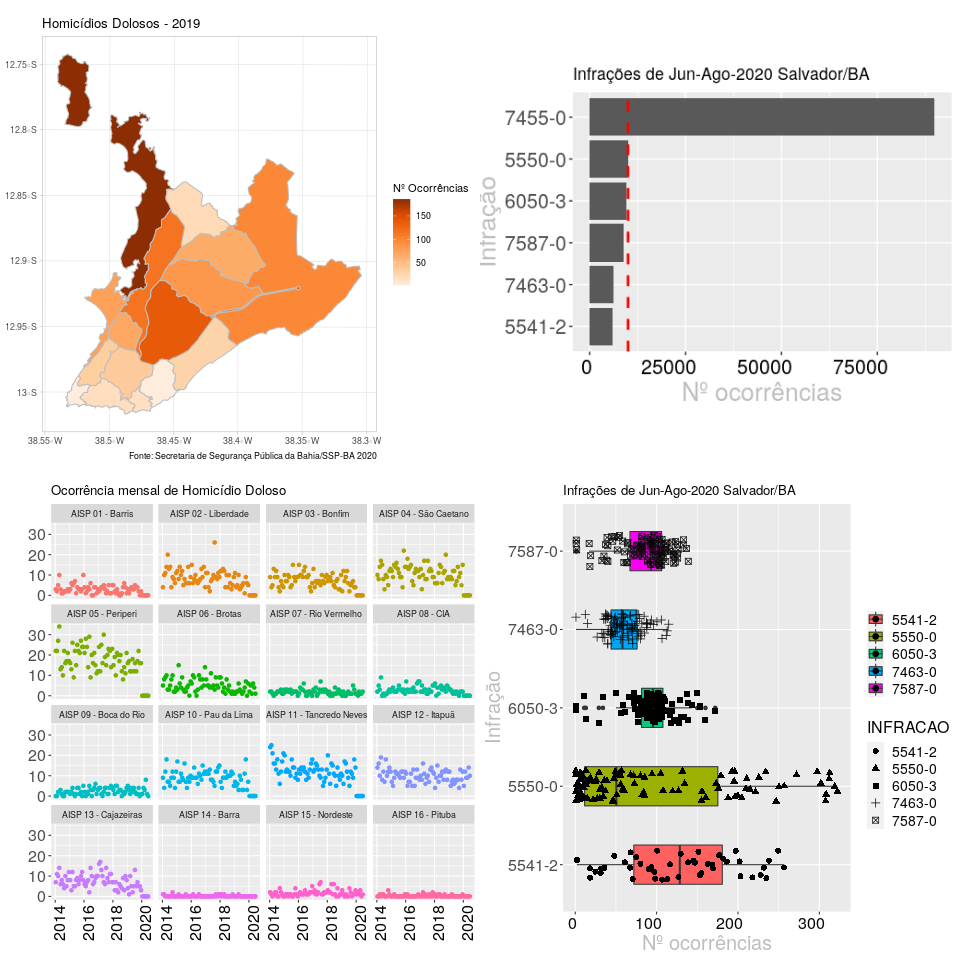
\includegraphics[width=13.33in]{images/imagereunida} \caption{Exploração dos temas de Segurança Pública e de Mobilidade Urbana.}\label{fig:reunicossa}
\end{figure}

\hypertarget{representauxe7uxe3o-gruxe1fica-dos-dados-e-desenvolvimento-dos-dashboards}{%
\section{Representação gráfica dos dados e desenvolvimento dos Dashboards}\label{representauxe7uxe3o-gruxe1fica-dos-dados-e-desenvolvimento-dos-dashboards}}

Para alcançar o desenvolvimento do ambiente de dados na forma gráfica mais apropriada para este estímulo ao conhecimento, exploramos a linguagem mais popular e de fácil implementação. Utilizamos os recursos da linguagem R, com dados na sua maioria disponibilizados no formato de csv. A linguagem R é capaz de trabalhar com um recurso amplo de ferramentas, entre suas principais qualidades está a programação com markdown. Entre as vantagens de se trabalhar com markdown no R está a produção de textos, documentos, livros e websites com estruturas muito simples de programação e a possibilidade de produção de saídas em html. Essas saídas podem ser configuradas com programação via linguagem css. Outras importante característica está na forte integração com outras linguagens amplamente utilizadas na área de ciência de dados como Python, Julia, C++ e SQL. Quando se trabalha com estas fontes de programação atuamos para o benefício de um fim público com custo muito baixo, prática muito comum da área de software livre. A linguagem R tem a seu dispor uma importante ferramenta para a produção de APIs, Shiny. Especialmente nesta estrutura é possível produzir interfaces para que o usuários seja capaz de fazer filtros, definir faixas de apresentação de informações, usufruir dos códigos de inferência do R com a flexibilidade de funcionamento em versão Desktop ou Mobile. Esta importante estrutura do R tem os elementos pré programados que aceleram a produção dessas interfaces de apresentação gráfica e interação com o usuário. Há ainda no R uma estrutura de código para produção de interfaces mais simples chamada de Flexdashboard com a vantagem de ser facilmente integrável a estruturas de sites produzidos em Wordpress.
Para o desenvolvimento dos dashboards foi optado pelo controle de versões realizado via Github na conta do projeto \href{https://github.com/orgs/cienciadedadosnaep/}{Ciência de Dados na Escola Pública}. O ambiente do github permite a publicação do do dashboard na forma de website desde que o repositório desenvolvido esteja no modo público. Assim é possível ao mesmo tempo, produzir o dashboard, realizar controle de versões, permite a integração com o desenvolvimento da Website e mantém o padrão da política de dados abertos. A disponibilidade do código dos dashboards em formato aberto tem entre outras vantagens a fácil difusão do conhecimento para que outras cidades que desejem aderir à proposta de reconhecimento das suas cidades por meio de dados. Para alguns tipos de dados como pirâmide etárias ou dados desagregados por faixa etárias foi utilizado um formato no qual o controle de versões é realizado por meio do Github porém a publicização do dashboard foi realizado no repositório Appshiny. As Figuras \ref{fig:dashm1cossa} a \ref{fig:dashm3cossa} são a representação de um dos \href{https://robsonpessoa.shinyapps.io/piramide_etaria/}{dashboards} desenvolvidos para uso do website. A Figura \ref{fig:dashm1cossa} demonstra a estrutura geral do dashboard que inclui uma estrutura de seleção da classe, que funciona como filtro para o banco de dados que são utilizados na renderização do gráfico. Esta estrutura foi desenvolvida utilizando o Flexdashboard com elemento de entrada sendo incluindo como uma funcionalidade do pacote Shiny, no preâmbulo do Flexdashboard é utilizada a linguagem yaml e assim é possível integrar estes pacotes (runtime: shiny). A Figura \ref{fig:dashm2cossa} dá destaque ao sistema de seleção com barra de rolagem. No corpo principal foi utilizado o pacote dplyr do R para gestão dos dados enquanto as figuras foram produzidas por meio do ggplot2. Algumas funcionalidades como zoom, destaque de áreas, impressão da visualização atual do gráfico e o recurso mouseover obtido pela aplicação do pacote ggplotly, na figura \ref{fig:dashm3cossa}, no canto superior direito é possível ver os botões destes recursos. Também foi testado o pacote echarts4r, com sua base em Java Script, tem forte integração com o pacote dplyr. Embora tenha uma estética simples e agradável e bom comportamento, não tem a mesma variedade de opções gráficas que ainda será necessária em futuras modificações do website.

\begin{figure}
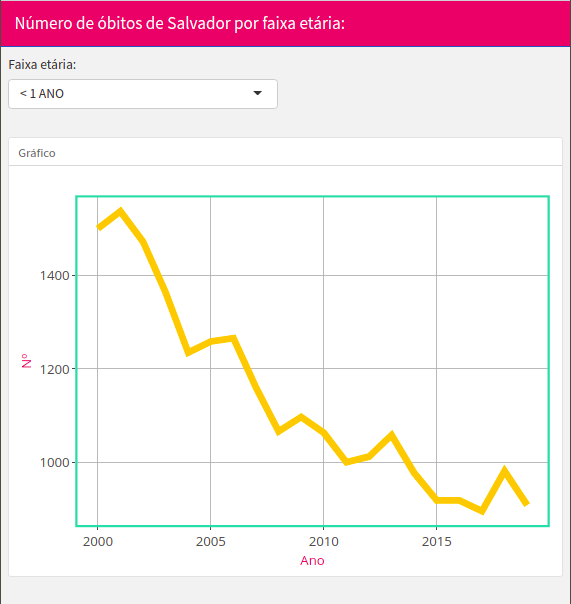
\includegraphics[width=7.93in]{images/image65} \caption{ Dashboards  com dados de número de óbitos anuais de Salvador apresentados em gráficos de linha e caixa de seleção de classe.}\label{fig:dashm1cossa}
\end{figure}

\begin{figure}
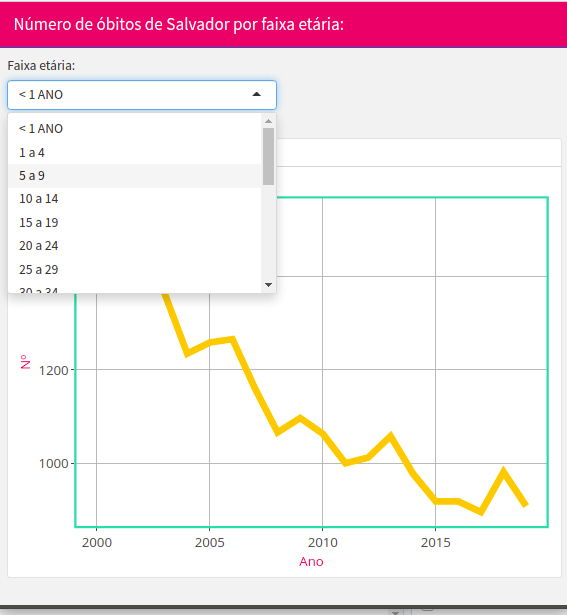
\includegraphics[width=7.88in]{images/image6} \caption{Destaque da caixa de seleção de faixas etárias.}\label{fig:dashm2cossa}
\end{figure}

\begin{figure}
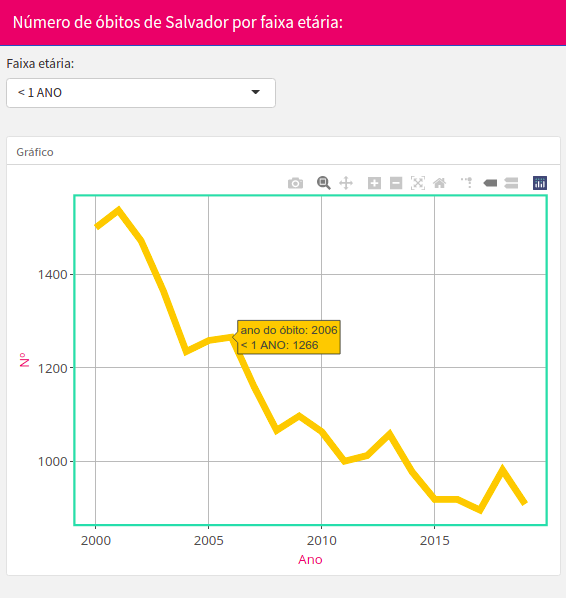
\includegraphics[width=7.86in]{images/image82} \caption{Destaque para o comportamento de resposta do gráfico ao movimento do ponteiro do mouse.}\label{fig:dashm3cossa}
\end{figure}

Também com intuito de exemplificar os dashboards desenvolvidos, demonstramos na Figura \ref{fig:dashm4cossa} construída de forma estática, ou seja, sem recursos Shiny, a possibilidade de criar uma estrutura que ao invés de filtrar dados temos as diferentes variáveis dispostas num sistema de abas com destaque em amarelo para aquela que está em uso.

\begin{figure}
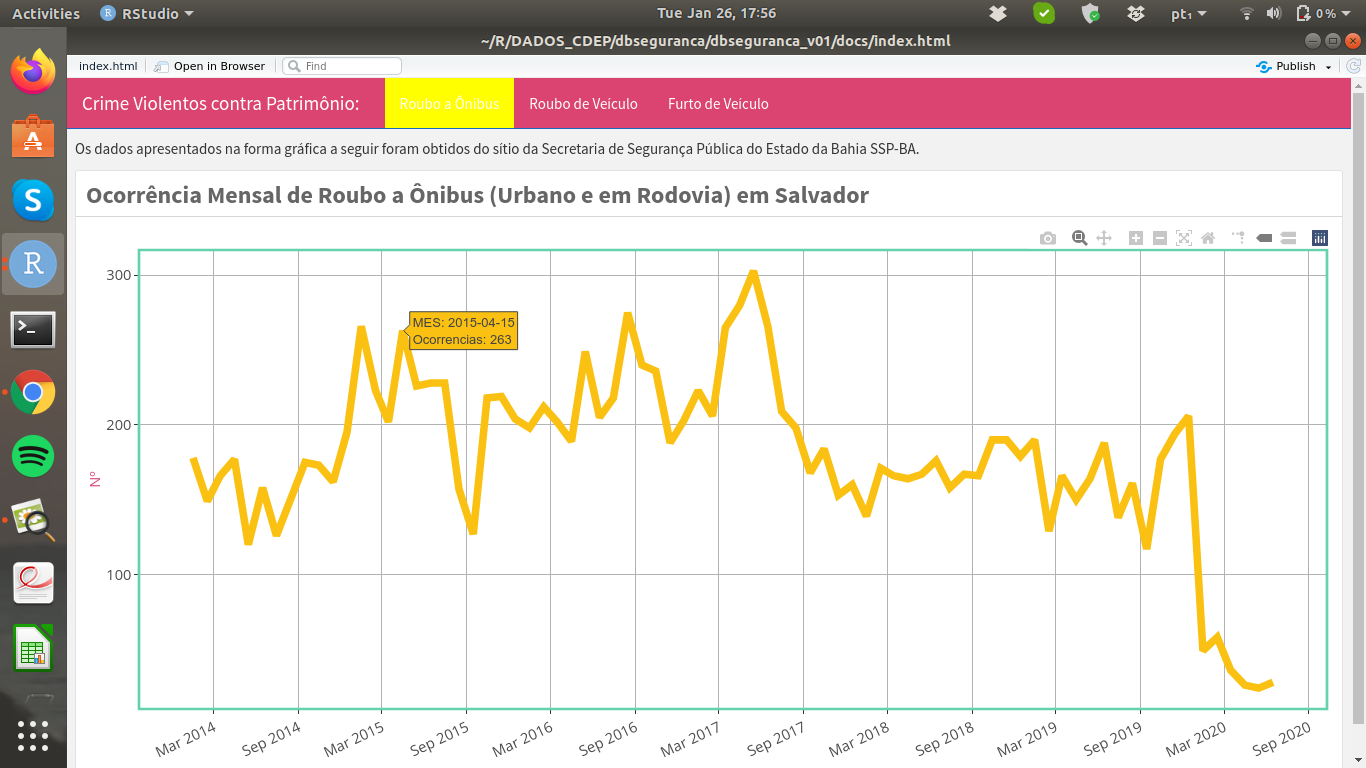
\includegraphics[width=18.97in]{images/image9} \caption{Dashboard de Crimes Violentos contra o Patrimônio, é formado por 3 abas com séries temporais dos crimes Roubo à ônibus (destacada em amarelo), Roubo de Veículo e Furto de Veículo.}\label{fig:dashm4cossa}
\end{figure}

A opção de diferentes formas gráficas e diferentes disposições do dashboard ocorre de acordo com o tipo de variável e nível de dificuldade apropriado ao estudante, vejamos os dados de população apresentada na Figura \ref{fig:dashm5cossa}. Neste dashboard foi optado pela forma gráfica recorrente no ensino fundamental para apresentação de informações por faixa etária e pirâmide etária. Ao lado da pirâmide etária é apresentado o levantamento histórico do número de pessoas residentes em Salvador desde o século XVI.

\begin{figure}
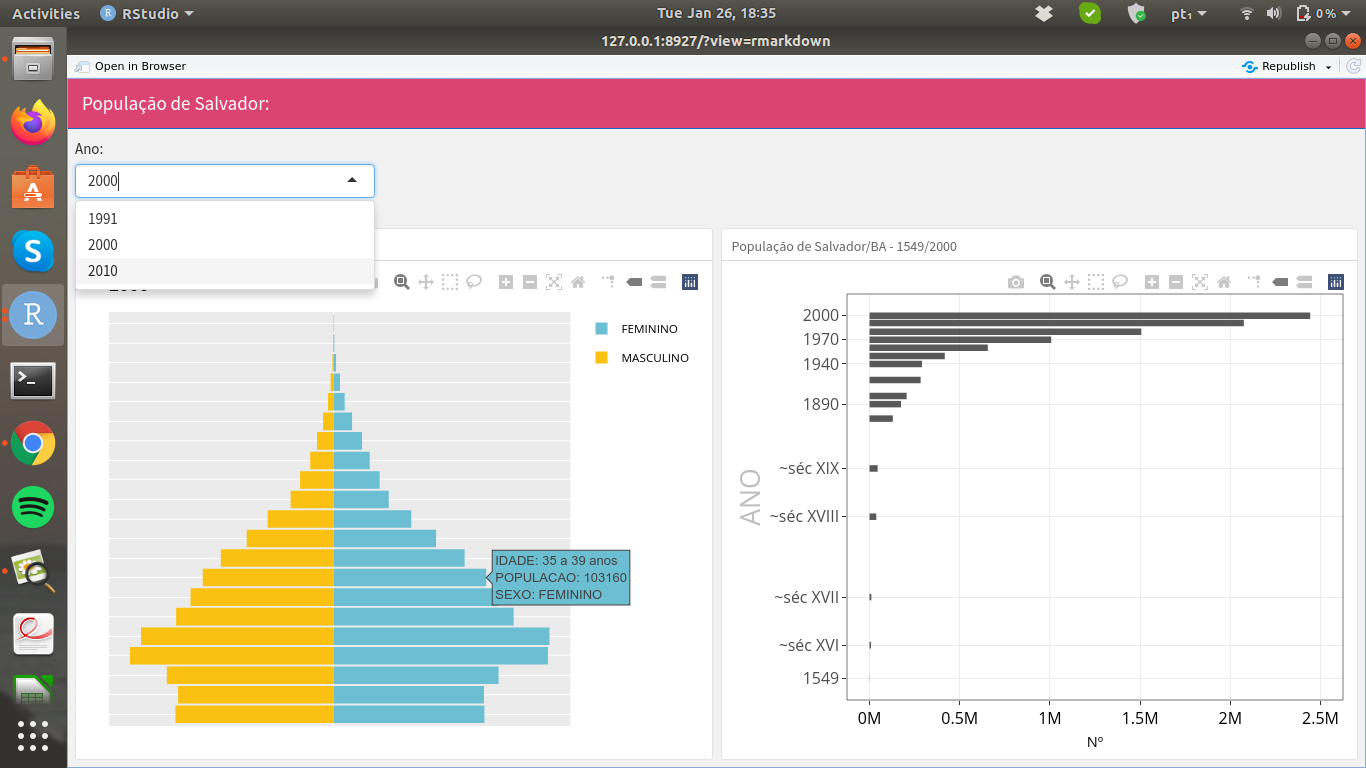
\includegraphics[width=18.97in]{images/image51} \caption{Dashboard de população com dados do Censo de 1991, 2000 e 2010 disponíveis como pirâmide etário e do lado direito a evolução da população de Salvador a partir do século XVI.}\label{fig:dashm5cossa}
\end{figure}

\hypertarget{desenvolvimento-e-acesso-de-novos-muxe9todos-e-metodologias-de-ensino-e-aprendizagem}{%
\chapter{Desenvolvimento e acesso de novos métodos e metodologias de ensino e aprendizagem}\label{desenvolvimento-e-acesso-de-novos-muxe9todos-e-metodologias-de-ensino-e-aprendizagem}}

Nos meses de novembro e dezembro de 2020 pretende-se realizar estudos avançados em metodologias de ensino voltadas para a educação pública. Serão estudadas as metodologias desenvolvidas e utilizadas pela: (1) \href{https://preuss.ucsd.edu/}{Preuss School}, escola voltada para a formação de estudantes do ensino fundamental II e médio, de baixa renda, que se esforçam para se tornarem os primeiros em suas famílias a ingressarem na universidade e concluírem o nível superior. Localizado no campus da Universidade da Califórnia San Diego (UCSD), os estudantes têm a oportunidade de utilizar a estrutura universitária da UCSD e vivenciarem um ambiente que os incentiva a tomada de riscos intelectuais, oferecendo uma variedade de apoios acadêmicos. Quase 100\% dos seus estudantes ingressam e concluem o nível universitário, concorrendo com estudantes de escolas públicas e privadas; (2) \href{https://create.ucsd.edu/}{CREATE}, órgão da UCSD que apoia e promove projetos e ações educacionais visando o desenvolvimento de estudantes e a capacitação de professores, considerando suas necessidades locais, e promovendo o seu acesso à universidade; (3) Lemann Center for Educational Entrepreneurship and Innovation in Brazil da Universidade de Stanford, que apoia uma variedade de projetos de pesquisa e inovação, com foco na melhoria das oportunidades de aprendizagem para estudantes socialmente desfavorecidos dentro e fora do sistema público de ensino; (4) \href{https://www.youcubed.org/}{You Cubed da Universidade de Stanford}, grupo de pesquisa cujos projetos visam inspirar, educar e capacitar professores de matemática e transformar as recentes pesquisas sobre matemática em formas acessíveis e práticas; (5) \href{https://tltlab.org/}{Transformative Learning Technologies Lab (TLTL) da Universidade de Columbia}, grupo multidisciplinar que projeta e pesquisa novas tecnologias para a educação. Ao final, pretende-se construir propostas de ferramentas e metodologias considerando a realidade do público escolar que faz parte do projeto e das escolas públicas de Salvador e da Bahia. Até então, os seguintes contatos foram realizados:

\begin{itemize}
\tightlist
\item
  Reunião presencial e troca de e-mails com Tamika Franklin- Diretora de Desenvolvimento da Preuss School. Apresentação do projeto e propostas de futuras parcerias (pós-pandemia), 10/03/2020.
\item
  Participação do Lemann Center Virtual Meeting da Stanford University. Apresentação dos projetos Meninas na Ciência de Dados e Ciência de Dados na Educação Pública a convite de um dos seus diretores, Prof.~Eric Bettinger, 29/09/2020.
\item
  Reunião virtual com Raquel Coelho, doutoranda em International Compatative Education and in Learning Sciences and Technology Design do Lemann Center for Educational Entrepreneurship and Innovation in Brazil, 14/10/2020.
\item
  Reunião virtual com Tatiana Hochgreb-Haegeke e Guilherme Desiderio, responsáveis pelo Programa de Especialização Docente Brasil (PED Brasil), apoiado pela Stanford University em parceria com instituições de ensino superior brasileiras, 19/01/2020.
\end{itemize}

\hypertarget{desenvolvimento-do-pensamento-cientuxedfico}{%
\chapter{Desenvolvimento do pensamento científico}\label{desenvolvimento-do-pensamento-cientuxedfico}}

As atividades relacionadas ao desenvolvimento do pensamento científico envolvem a construção do E-book (relatado na sessão 1), o fortalecimento do pensamento científico das/os estudantes nos encontros virtuais e a sua mobilização para que participem de eventos científicos.
Tais atividades se baseiam em três eixos estruturantes da alfabetização científica: (a) Compreensão básica de termos e conceitos científicos, em que são trazidos aos estudantes elementos que compõem uma investigação científica (conhecimento); (b) Compreensão da natureza da ciência e os fatores que circundam sua prática, demonstrando a importância da investigação científica e sua diversidade (reconhecimento); (c) Compreensão das relações existentes entre investigação científica, tecnologia, sociedade e meio ambiente (aplicação).
O Quadro Colaborativo ilustrado na Figura \ref{fig:prodcocient} sintetiza os elementos associados ao pensamento científico trabalhados, destaca-se que esse quadro foi construído juntamente com as/os estudantes partícipes do Projeto.

\begin{figure}
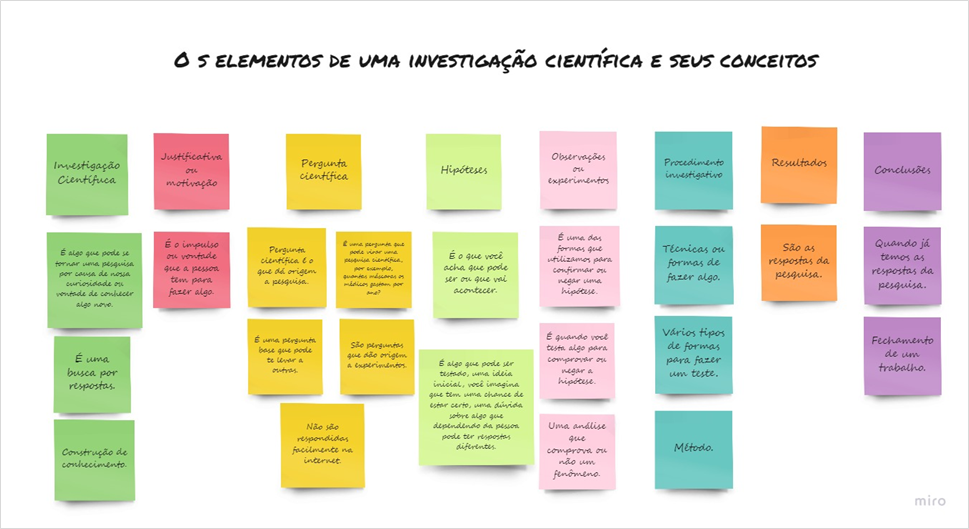
\includegraphics[width=13.46in]{images/image105} \caption{Quadro Colaborativo construído juntamente com os estudantes partícipes do Projeto.}\label{fig:prodcocient}
\end{figure}

A equipe identificou a oportunidade, durante o período das atividades, de incentivar e oferecer apoio à inscrição dos estudantes de escolas públicas em dois eventos científicos distintos: 10º Evento Jovens Cientistas da UFBA (Tabela \ref{tab:quadro1}); e a Feira de Ciências do Agreste Pernambucano - FCAP (Tabela \ref{tab:quadro2}), como forma de desenvolver na prática os conceitos explorados nos encontros e no material didático em produção, bem como seus respectivos links de acesso.

\begin{table}

\caption{\label{tab:quadro1}Resumos submetidos à Revista Jovens Cientistas da UFBA – 2020}
\centering
\begin{tabular}[t]{l|l|l}
\hline
Escola & Estudante & Título do resumo\\
\hline
Colégio Estadual Evaristo da Veiga & Ana Paula Santos Pinheiro & Minha visão da pandemia como estudante\\
\hline
 & Ana Vitória de Jesus Silva & Convivendo a pandemia\\
\hline
 & Gabrielle Santos Pinheiro & Como eu tenho estado em meio a essa tempestade que estamos passando\\
\hline
 & Jaqueline Santos Barbosa & Reflexões sobre a pandemia\\
\hline
Colégio Henriqueta Martins Catharino & Amanda Jesus Borges dos Santos & A pandemia\\
\hline
 & Ana Beatriz Santos de Jesus & Nota com café\\
\hline
 & Pâmella Brendha Santos da Silva & O mundo em luto\\
\hline
Colégio Municipal Cidade de Jequié & Carrolyne Santos Dourado & Pandemia, só que para estudante\\
\hline
 & Karin Beatriz da Silva Souza & Desabafo\\
\hline
 & Maria Eduarda Menezes de Nascimento & Mudança de vida\\
\hline
Colégio Estadual Mário Costa Neto & Vitória Nascimento de Jesus & Minha vida na quarentena\\
\hline
Colégio Estadual Ypiranga & Gabrielle Tereza dos Santos & O meu relato da quarentena\\
\hline
 & Isabele Xavier da Silva Barros & Eu e minha 40tena\\
\hline
 & Maria Thainá Mota da Silva & Rotina de um isolado\\
\hline
 & Marisa Jheymille da Silva Cabral & A pandemia\\
\hline
\end{tabular}
\end{table}

Os resumos foram revisados por um dos membros da equipe, com foco apenas em adequações de língua portuguesa, e, depois, foram submetidos pela equipe à revista.

\begin{table}

\caption{\label{tab:quadro2}Projetos submetidos e aprovados na Feira de Ciências do Agreste Pernambucano e links de acesso dos vídeos apresentados.}
\centering
\begin{tabular}[t]{l|l|l|l}
\hline
Escola / Professores responsáveis & Estudantes & Temas dos Projetos Científicos & Links dos vídeos apresentados\\
\hline
Colégio Estadual Evaristo da Veira / Erica Nascimento e Allena Araújo & Ana Paula Santos Pinheiro e Gabrielle Santos Pinheiro & Densidade de Sólidos e de Fluidos de um Campo de Petróleo: Determinação Experimental e Simulação Interativa & https://fb.watch/1gkqy8iag1/\\
\hline
 & Ana Vitória de Jesus Silva e Jaqueline Santos Barbosa & Medição do pH de soluções utilizando diferentes métodos experimentais e simulação interativa & https://fb.watch/1glpFnL8f3/\\
\hline
Colégio Estadual Ypiranga / Maysa Cavalcante Lima e Yone Santiago & Isabela Xavier da Silva Santos e Maria Thainá Mota da Silva & Rotina dos alunos do CEY na pandemia & https://www.facebook.com/watch/?v=830047974428506\\
\hline
 & Gabrielle Tereza dos Santos e Marisa Jeymille da Silva Cabral & Adubo Orgânico Caseiro & https://www.facebook.com/watch/?v=392835515207156\\
\hline
Colégio Estadual Henriqueta Martins Catharino / Alzira Melo e Cláudia Cajado & Cailane Lima de Jesus e José Carlos Archanjo de Jesus & Os postos de saúde e a qualidade do atendimento à população & https://www.facebook.com/watch/?v=1560201997515180\\
\hline
 & Igor Moreno Dórea Pinheiro dos Santos e Marcos Vinícius Carvalho Costa & Robótica – Helicóptero movido a energia solar & Vídeo não apresentado\\
\hline
\end{tabular}
\end{table}

Participaram dessa atividade, além das estudantes bolsistas, uma estudante que fez parte dos encontros formativos e informativos nas escolas em 2019, Cailane Jesus, e estudantes do sexo masculino, recém ingressos no projeto. Os projetos de ciências produzidos pelas estudantes do Colégio Estadual Evaristo da Veiga são frutos de uma parceria estabelecida com o Laboratório de Petróleo e Gás -- LAPEG, iniciada em 2019; apresentam, portanto, conteúdo ligado a ciências/química. Os projetos produzidos pelas/os estudantes do Colégio Estadual Ypiranga e Colégio Estadual Henriqueta Martins Catharino destacam-se pelo caráter social ou ambiental dos temas trabalhados, temas que foram selecionados pelas/os próprias/os estudantes.

\hypertarget{encantamento-e-capacitauxe7uxe3o-de-professores}{%
\chapter{Encantamento e capacitação de professores}\label{encantamento-e-capacitauxe7uxe3o-de-professores}}

\hypertarget{encontros-virtuais-com-professorases-cafuxe9-com-dados}{%
\section{Encontros virtuais com professoras/es (Café com Dados)}\label{encontros-virtuais-com-professorases-cafuxe9-com-dados}}

Encontros virtuais abertos a professores e comunidade escolar das cinco escolas participantes do projeto, bem como toda a sociedade ocorreram através do Café com Dados. Os encontros totalizaram uma carga horária aproximada de 40h, dividida em encontros de uma vez por semana, que duravam entre 1h a 1h30. As gravações dos encontros estão disponíveis no \href{https://cienciadedadosep.wixsite.com/cafecomdados}{site do projeto}, possibilitando, assim, que as discussões alcançassem pessoas que não estavam presentes nos momentos dos encontros. A primeira etapa, realizada de abril a julho de 2020, visou encantar e aproximar os professores e coordenadores das escolas ao tema de ciência de dados e suas relações com os demais temas (inteligência artificial, produção do conhecimento científico e protagonismos social, racial e de gênero). A segunda etapa ocorreu de agosto a outubro, no formato de mediações didáticas. Nestes encontros foram apresentados e discutidos os conteúdos trabalhados nos encontros virtuais com as/os estudantes liderados pela equipe do projeto.

\textbf{Abril 2020}
Desmistificando a ciência de dados - Profa. Karla Esquerre / UFBA; Ciência de dados na Engenharia de transportes - Prof.~Jorge Ubirajara / UFBA; Ressignificando os dados públicos sobre COVID-19: As iniciativas não governamentais - Fernando Barbalho / Tesouro Nacional; Testes diagnósticos para o COVID - 19 - Profs. Danilo Klein e Alexandre Silva / UERJ e Secretaria Extraordinária de Acompanhamento das Ações Governamentais Integradas do Covid 19 do Rio de Janeiro; Ferramentas online para suporte ao ensino - Ana Carolina Santos, Ana Luisa Nogueira, Janaina Souza, Thalita Senna e Profa. Karla Esquerre / UFBA.

\textbf{Maio 2020}

Ciência de dados na educação pública - Profa. Karla Esquerre / UFBA; Webinar: explorando um Design Universal de Aprendizagem em Programação; Pensamento Computacional - Geisa Santos / IAT; Jurimetria - Julio Trecenti; Ciência de Dados no esporte - Prof.~Daniel Takata Gomes

\textbf{Junho 2020}

Hackers na Educação - Profa. Karina Menezes / UFBA; Pesquisa em segurança pública em evidências: O caso das delegacias das mulheres - Prof.~Sandro Cabral / UFBA - Insper; A robótica transformando a educação e as pessoas - Profa. Andrea Bittencourt / IFBA; Interpretando dados para compreender fenômenos biologicamente complexos-efeitos analgésicos de células-tronco - Profa. Cristiane Flora Villarreal / UFBA

\textbf{Julho 2020}

Debatendo sobre gênero e diversidade - Profa. Maíse Zucco / UFBA; Refletindo sobre o campo dos estudos de gênero e as contribuições para uma educação inclusiva - Profa. Maíse Zucco / UFBA; A versatilidade de um cientista de dados - Gabriela de Queiroz IBM / IA Inclusive; Ações da Fundação Itaú Social na área de educação - Renato Brizzi / Fundação Itaú Social; Algoritmos e pandemia: Fatos biológicos e ficções culturais - Profa. Jamile Borges / UFBA; Educação para justiça social: Conceito e métricas - Icaro Bernardes / UFBA (Set 2020).

Contribuíram como palestrantes professores, profissionais, estudantes de graduação e pós-graduação compartilhando as suas experiências nas mais diversas áreas. Destaca-se a participação das professoras Alzira Melo e Érica Nascimento, do Colégio Estadual Henriqueta Martins Catharino e do Colégio Estadual Evaristo da Veiga, respectivamente, que apresentaram suas experiências ministrando a disciplina Introdução à Inteligência Artificial juntamente com a graduanda Ana Luisa Nogueira e a mestranda Laís Bastos, ambas bolsistas do projeto. A Figura \ref{fig:cafe} apresenta um registro desse encontro.

\begin{figure}
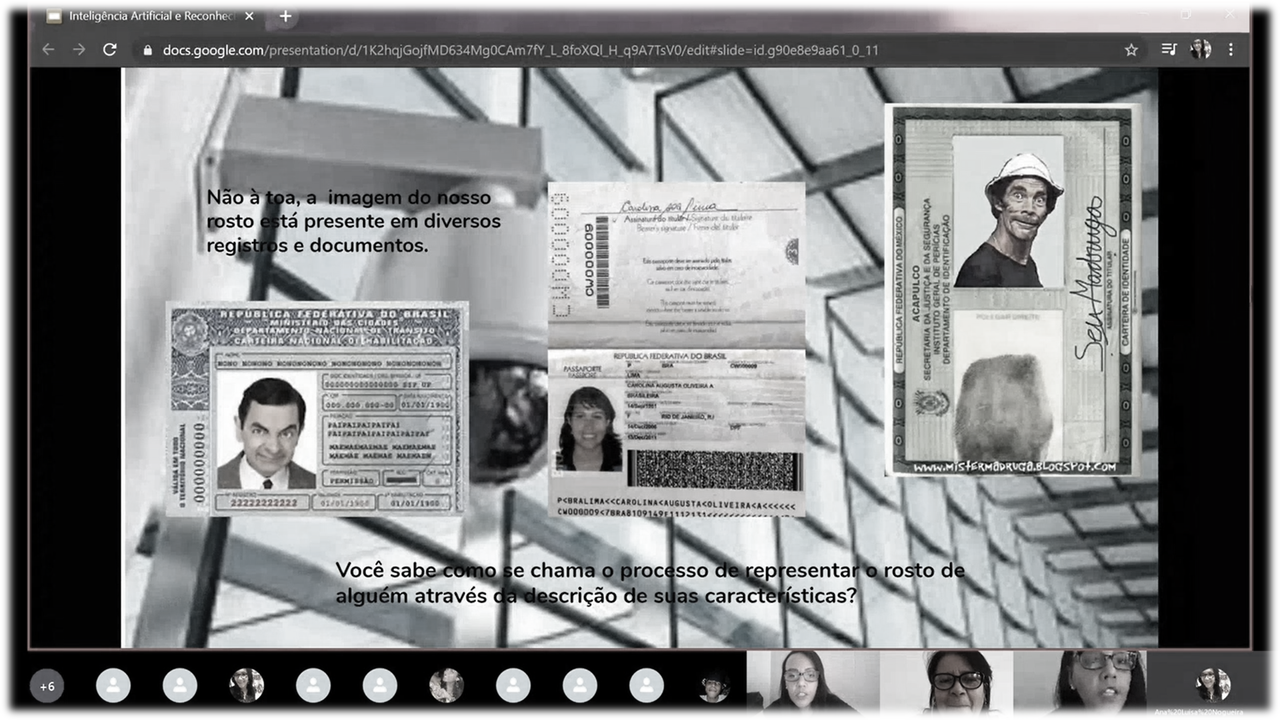
\includegraphics[width=17.78in]{images/image121} \caption{Registro do encontro da disciplina Introdução à Inteligência Artificial em 01 de setembro, com o tema Reconhecimento Facial.}\label{fig:cafe}
\end{figure}

\hypertarget{construuxe7uxe3o-da-disciplina-inteliguxeancia-artificial}{%
\section{Construção da disciplina Inteligência Artificial}\label{construuxe7uxe3o-da-disciplina-inteliguxeancia-artificial}}

Considerando a natureza eletiva de parte das disciplinas oferecidas no ensino médio, o Colégio Estadual Henriqueta Martins Catharino, na pessoa da professora Alzira Melo, propôs a oferta de uma disciplina na área de Ciência de Dados. De forma a atrair a atenção e interesse das/os estudantes, juntamente com a equipe do projeto foi proposta a disciplina de Inteligência Artificial. Além desse colégio, o Estadual Evaristo da Veiga, na pessoa da professora Érica Nascimento, propôs oferecer a mesma disciplina. Uma proposta de ementa foi elaborada no início de 2020.
A aproximação dessas professoras ao tema de Inteligência Artificial foi iniciada através da produção de textos/resumos baseados em artigos científicos, vídeos, reportagens e cursos relacionados a esses temas. Tal atividade foi conduzida por um membro do projeto vinculado à equipe de protagonismo. No total, foram elaborados 02 resumos baseados em vídeo conferências, 02 resumos baseados em artigos científicos, 01 resumo baseado em vídeo reportagem e 10 resumos baseados em reportagens de revistas e jornais online. As referências utilizadas para a produção dos resumos são apresentadas na Sessão Bibliográfica. A lista de resumos é apresentada no Apêndice 12.2 e os resumos completos podem ser acessados no \href{https://drive.google.com/drive/folders/1J2h6ljxDrwNOSu66Wzr-V13JCXEHWzHv?usp=sharin}{Drive}.

Inicialmente, a equipe de Inteligência Artificial iria apenas apoiar as professoras e instituições na disciplina. No entanto, por ter que ser conduzida de modo virtual, foram percebidas as necessidades de adaptar a ementa inicialmente proposta para a quantidade de encontros previstos e para a dinâmica de um encontro virtual. Assim, ficou acordado que seriam realizados encontros semanais dentro do período de 18 de agosto a 24 de novembro de 2020. Aliado ao discurso das professoras que se mostraram inseguras em alguns pontos da liderança do encontro, também ficou definida a alternância quinzenal da liderança desses encontros com a equipe do projeto. Nos encontros liderados pelas professoras, passaram a ser abordadas as aplicações e implicações da inteligência artificial enquanto a equipe do projeto passou a se dedicar aos tópicos mais teóricos e conceituais. Nos encontros das professoras, elas utilizaram a experiência adquirida com a produção dos resumos para propor os temas e discussões dos seus encontros. Para a discussão dos tópicos e de eventuais dúvidas das professoras, também ficaram combinadas reuniões semanais ou quinzenais com as professoras e uso do grupo do WhatsApp para diálogos e compartilhamentos. A ementa da disciplina é apresentada no Apêndice 12.3.
As inscrições para a disciplina foram feitas através de um formulário do Google compartilhado com um card para divulgação da iniciativa. O link foi divulgado pelas professoras e coordenadoras entre os estudantes e foi divulgado pela equipe do projeto entre os estudantes bolsistas.
Ao todo, foram feitas 43 inscrições. Contudo, 20 estudantes nunca compareceram. Essas faltas foram averiguadas e, geralmente, apresentaram justificativas relacionadas à pandemia. Foi observada uma frequência máxima de 23 estudantes no encontro do dia 01/09/2020, e mínima de 11 estudantes no encontro do dia 13/10/2020, variando entre esses valores e entre os mesmos estudantes. Vale ressaltar que temos estudantes sem faltas.
Na Figura \ref{fig:diagramaAI} é apresentada uma representação das discussões de Inteligência Artificial e a formação de futuros protagonistas de transformação da sociedade.

\begin{figure}
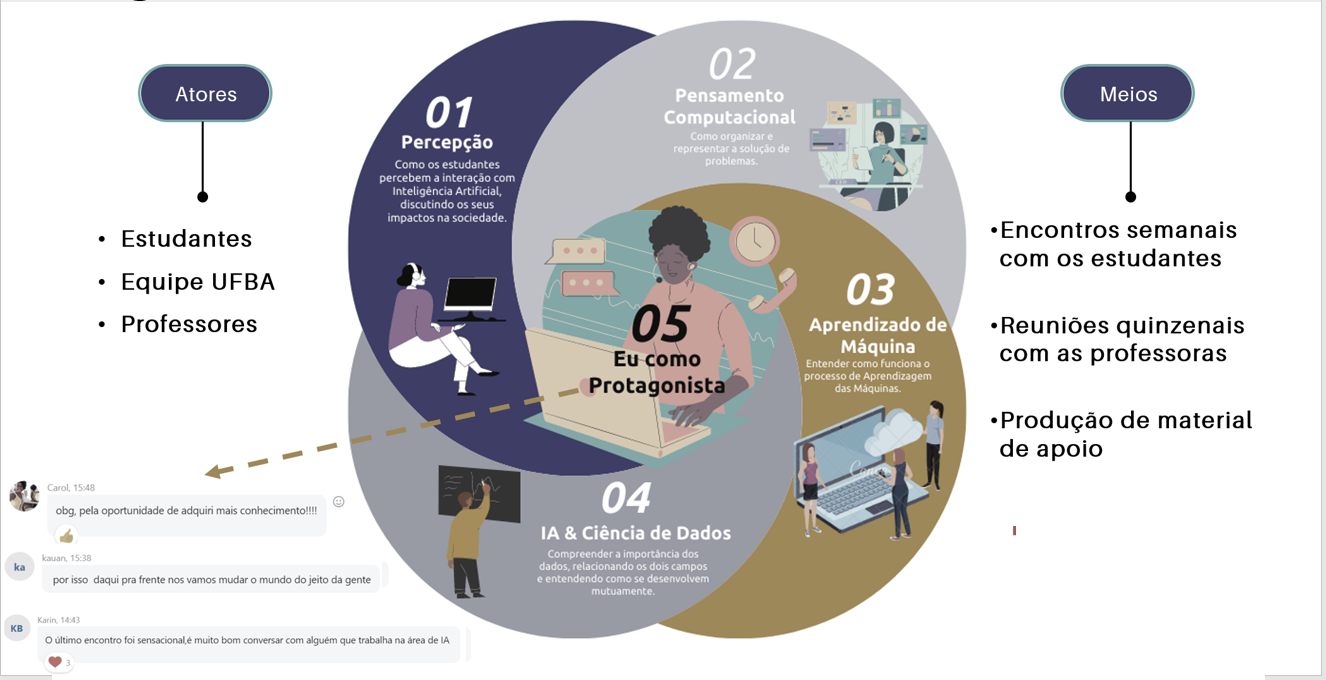
\includegraphics[width=18.42in]{images/image123} \caption{Discussão dos vários aspectos da IA e os resultados na formação de protagonistas de transformação da sociedade. Textos no extremo esquerdo: “obg pela oportunidade de adquirir (sic) mais conhecimento!!!”; “por isso daqui pra frente nós vamos mudar o mundo do jeito da gente”; “o último encontro foi sensacional, e muito bom conversar com alguém que trabalha na área de IA”.}\label{fig:diagramaAI}
\end{figure}

\hypertarget{construuxe7uxe3o-de-uma-parceria-com-professorases-do-iat}{%
\section{Construção de uma parceria com professoras/es do IAT}\label{construuxe7uxe3o-de-uma-parceria-com-professorases-do-iat}}

No dia 14/12/2020, a equipe de protagonismo realizou uma reunião com quatro professores e uma coordenadora de uma escola pública no interior da Bahia. A reunião teve como objetivo promover a escuta dos professores e levantar suas expectativas sobre parceria com Projeto Ciência de Dados na Educação Pública com vistas a elaborar proposta conjunta de ação para estimular o protagonismo juvenil em sala de aula segundo uma perspectiva transdisciplinar em suas respectivas escolas.
Durante a reunião, as integrantes da equipe de protagonismo convidou os professores participantes a preencherem coletivamente e online um material contendo as questões abaixo:

\begin{itemize}
\tightlist
\item
  Qual a importância do protagonismo juvenil?
\item
  Por que o protagonismo juvenil deve ser inserido no currículo escolar?
\item
  Qual o perfil dos alunos com quem eu trabalho?
\item
  Quais as expectativas em relação ao trabalho em parceria com a equipe do Projeto Ciência de Dados na Educação Pública?
\end{itemize}

As respostas dos professores estão disponíveis neste \href{https://pad.riseup.net/p/CDnaEP}{link da pasta}.
Os professores manifestaram interesse em rever e dar nova roupagem a projetos já existentes na escola (ex. experiência da Aprendizagem Criativa), às disciplinas eletivas nas quatro grandes áreas (ex. Itinerário Formativos) e outras não eletivas. Há receptividade em relação ao engajamento e à formação dos demais professores para construir coletivamente as estratégias, ao invés de levar propostas prontas, definidas sem sua participação.
Ao final, foi firmada a manutenção do contato dos professores com a equipe do projeto prevista para 2021, considerando a manutenção do contexto pandêmico e incertezas das diretrizes do ensino nas escolas estaduais.

\hypertarget{encontros-virtuais-com-estudantes-bolsistas}{%
\chapter{Encontros virtuais com estudantes bolsistas}\label{encontros-virtuais-com-estudantes-bolsistas}}

\hypertarget{metodologia}{%
\section{Metodologia}\label{metodologia}}

A preparação do material para os encontros com as/os estudantes requereu a realização de pesquisa sobre o tema, a elaboração de slides, a discussão e elaboração de planos de aula, bem como a preparação de disparadores complementares (jogos, cards etc.). Para cada encontro, estima-se um tempo médio de dedicação da equipe correspondente a 8h.

A metodologia desenvolvida buscou a motivação e o engajamento das/os partícipes, tornando cada um/a protagonista do processo, através da mediação dos saberes. A construção de saberes está baseada, especialmente, nas metodologias ativas, com o estímulo para que as/os estudantes aprendam através de desafios sobre temas atrelados à ciência de dados, inteligência artificial, conhecimento científico e questões transversais, como gênero, raça e sociedade. Assim, há um esforço da/o estudante para propor possíveis soluções para os problemas trazidos pelas/os facilitadoras/es de modo colaborativo, a fim de instigar um perfil crítico, reflexivo e investigativo, conscientizando a construção do conhecimento.

Para o estudo de cada conteúdo, a/o estudante tem acesso antecipadamente a materiais -- textos, vídeos, imagens, histórias em quadrinhos etc. - sobre o tema a ser apresentado a cada encontro. Tal atitude busca instigar dúvidas, despertar o desejo de pesquisar mais sobre o assunto, dialogar com as/os colegas, contribuindo, assim, para a formação de sujeitos que fazem a diferença em seu contexto social.

Assim, o trabalho se apoia na construção de saberes dialógica e processual e na intertextualidade de linguagens audiovisuais distintas (poesias, fotos, músicas, vídeos, textos, pinturas etc.).
Todo o material elaborado para apoiar as atividades com os estudantes pode ser acessado em \href{https://cienciadedadosep.wixsite.com/estudantes}{}.
Encontros semanais com as/os estudantes
Iniciadas em 23/03/20, por conta da pandemia, as reuniões virtuais com as estudantes bolsistas do projeto eram realizadas uma vez por semana, com duração média de 60 minutos, utilizando ambientes virtuais de discussão gratuitos, acessados através do aplicativo Hangouts (disponível para computadores, tablets, laptops e celulares). Os encontros reuniram aproximadamente 15 a 20 estudantes, distribuídas em quatro subgrupos, cada qual conduzido por uma estudante de graduação membro do projeto. Em três destes grupos, houve a participação regular de três professoras oriundas das escolas parceiras. Os temas abordados nestes encontros eram voltados para a discussão de mulheres extraordinárias que mudaram o Brasil e o mundo, em continuação a uma atividade bastante apreciada pelas estudantes e iniciada no segundo semestre de 2019 de forma presencial. Como fruto dessas discussões, Podcasts foram produzidos por estudantes e postados inicialmente no YouTube e recentemente no \href{https://open.spotify.com/show/4hHoJYZVxVPOYrAT2OGuB8}{Spotify}.
Em agosto/2020, as distintas frentes de trabalho passaram a compor equipes específicas, responsáveis por conduzir reuniões temáticas correspondentes com as estudantes, considerando os eixos: Produção do Conhecimento Científico, Inteligência Artificial, Protagonismo e Ciência de Dados. Em paralelo, a metodologia anterior de realizar reuniões online com as alunas em pequenos grupos, organizados por escola, foi substituída pela organização de um único grupo reunindo todas as estudantes bolsistas.
A inclusão de estudantes do sexo masculino no projeto ocorreu também em agosto/2020, os quais não haviam participado do processo anterior de sensibilização das estudantes bolsistas. Assim, buscou-se estimular nas alunas uma postura receptiva e colaborativa diante dos recém-chegados, nos quais foram exercitados valores como respeito, cooperação, sensibilidade e adoção de posturas de combate às injustiças de gênero. Os conteúdos foram adaptados para promover a participação dos garotos nas discussões e entrosá-los aos demais colegas. Os ajustes se traduziram em uma nova abordagem sobre o protagonismo social, racial e de gênero, ampliando o foco anterior na atuação de determinadas figuras femininas para outros atores sociais.
Em 10/08/20, a equipe executora do projeto ampliou o tempo de contato/interação com os/as estudantes ao dar início à realização de duas reuniões semanais com as alunas, ao invés de apenas uma, como ocorria até o momento. Desde então, cada uma das cinco equipes de trabalho - o que inclui os profissionais responsáveis por organizar o site (Re)Conhecendo Salvador - se revezam na condução de encontros online com as/os estudantes.
Esses marcos temporais são úteis para compreendermos as mudanças ocorridas na condução e na periodicidade das reuniões online. Assim, entre 23/03/20 e 10/08/20, os encontros online foram realizados semanalmente, em subgrupos separados por escolas, sendo conduzidos por quatro facilitadoras distintas. Entre 10/08/20 e 21/12/20, os encontros passaram a ser realizados três vezes por semana, reunindo todas as estudantes em um único grupo, conduzido por 2 ou 3 facilitadoras/es de cada equipe. Na Tabela \ref{tab:quadro3} o número de encontros realizados por tema e sua associação com os e-books e site. A lista dos temas dos encontros com as/os estudantes é apresentada no Apêndice 12.3.

\begin{table}

\caption{\label{tab:quadro3}Encontros realizados com as/os estudantes.}
\centering
\begin{tabular}[t]{l|l|l}
\hline
Temas & Nº de encontros & E-book e capítulo associado aos assuntos discutidos\\
\hline
Protagonismo & 12 + 3 & Assuntos abordados diretamente ou tangencialmente no E-book 4\\
\hline
Ciência de Dados & 5 & E-book Ciência de Dados - Capítulos 1, 2, 6\\
\hline
Produção do Conhecimento Científico & 8 & E-book Produção do conhecimento científico - Capítulos - 1,2 e 3\\
\hline
(Re)Conhecendo Salvador / Exploração Gráfica & 4 & Site (re)Conhecendo Salvador - Temáticas: População, Turismo, Segurança Pública.\\
\hline
Inteligência Artificial & 9 & E-book Inteligência Artificial - Capítulos 1, 2, 3\\
\hline
\end{tabular}
\end{table}

\emph{12 encontros realizados de março a julho e 3 encontros realizados de agosto a outubro. Encontros da disciplina Inteligência Artificial, mas abertos a todos os estudantes bolsistas. 4 estudantes bolsistas do ensino fundamental II participam deste curso.}

Nas Figuras \ref{fig:meetenctprot} a \ref{fig:meetenctsite} são apresentados alguns registros desses encontros.

\begin{figure}
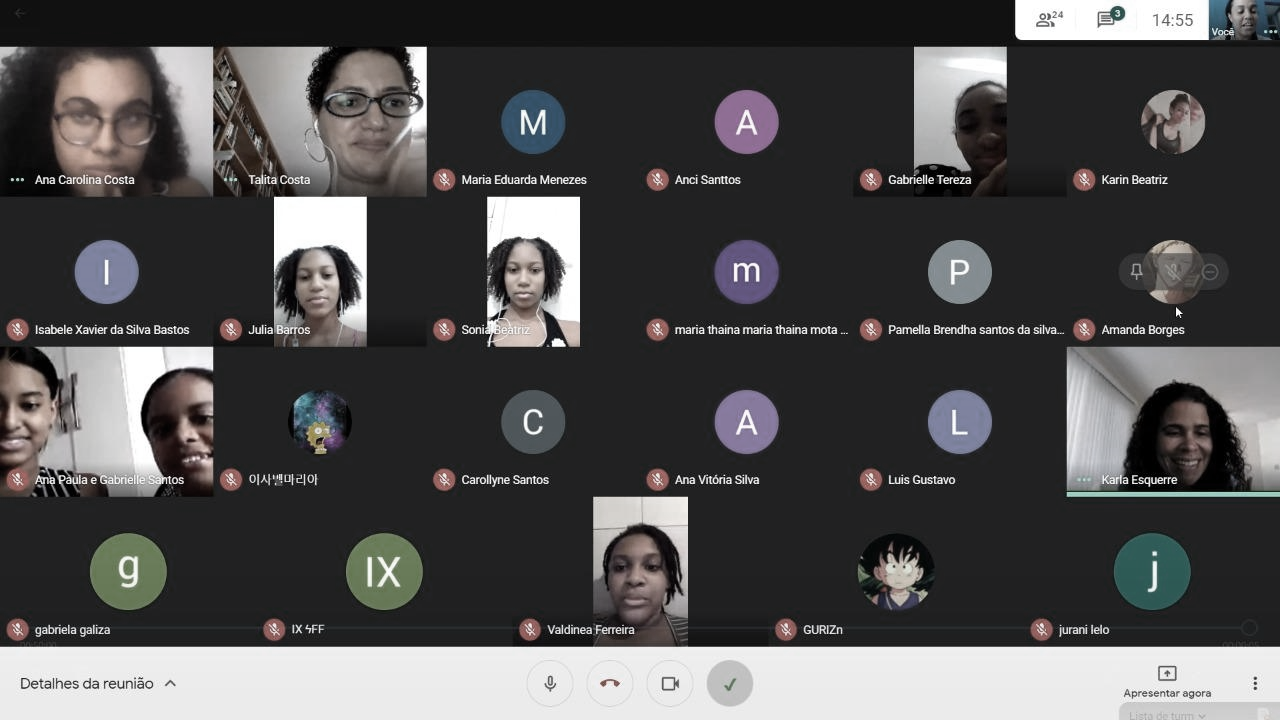
\includegraphics[width=17.78in]{images/image125} \caption{Registro de um dos encontros com a equipe de Protagonismo.}\label{fig:meetenctprot}
\end{figure}

\begin{figure}
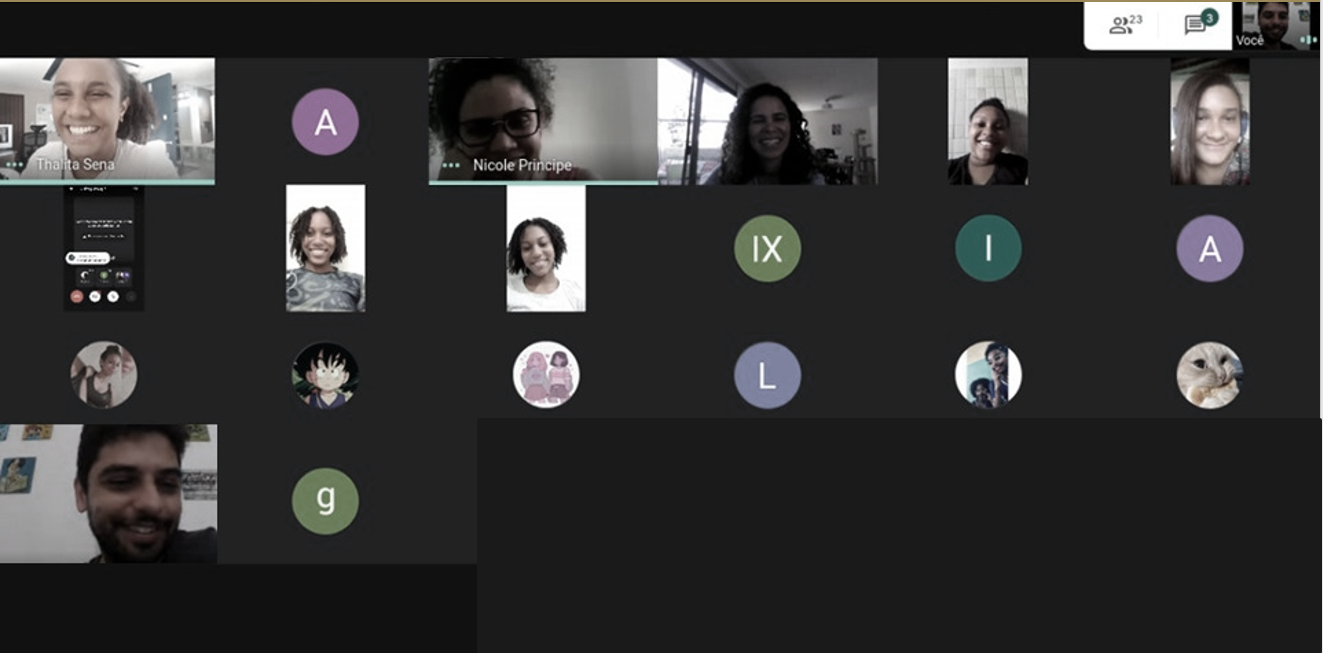
\includegraphics[width=18.38in]{images/image126} \caption{Registro de um dos encontros com a equipe do site (re)Conhecendo Salvador.}\label{fig:meetenctsite}
\end{figure}

\hypertarget{produuxe7uxe3o-de-podcasts-mulheres-extraordinuxe1rias}{%
\section{Produção de Podcasts: Mulheres Extraordinárias}\label{produuxe7uxe3o-de-podcasts-mulheres-extraordinuxe1rias}}

O objetivo desta atividade consistiu em fortalecer o protagonismo das estudantes; estimulá-las a mediar o aprendizado para seus pares e envolvê-los, ainda que indiretamente, nas ações do projeto.
Foi proposto às estudantes que, à distância, motivassem colegas (não vinculadas ao projeto) para produzir podcasts (áudios curtos passíveis de edição, disponibilizados via internet, dedicados a tratar de um tema específico) sobre as mulheres extraordinárias discutidas durante as reuniões do projeto, com base nos textos e pontos-chave elaborados pela equipe.
Cada episódio do podcast aborda a vida de três diferentes mulheres extraordinárias através dos áudios enviados pelas estudantes. Os temas dos podcasts produzidos pelas estudantes em 2020 são apresentados no Quadro \ref{tab:quadro4}. Eles podem ser acessados no \href{https://open.spotify.com/show/4hHoJYZVxVPOYrAT2OGuB8}{Spotify} (Figura \ref{fig:podcast}).

\begin{table}

\caption{\label{tab:quadro4}Podcasts produzidos pelas estudantes durante o período de abril a outubro de 2020.}
\centering
\begin{tabular}[t]{l|l|l}
\hline
Episódios & Data de publicação & Mulheres extraordinárias\\
\hline
4 & 03/06/2020 & Carolina Maria de Jesus, Antonieta de Barros e Maria Lenk\\
\hline
5 & 18/06/2020 & Dorina Nowill, Anne Frank, Graziela Maciel Barroso\\
\hline
6 & 20/08/2020 & Margarida Maria Alves, Indianara Siqueira e Jaqueline Góes\\
\hline
7 & 27/10/2020 & Sônia Guajajara, Malala, Djamila Ribeiro\\
\hline
\end{tabular}
\end{table}

\begin{figure}
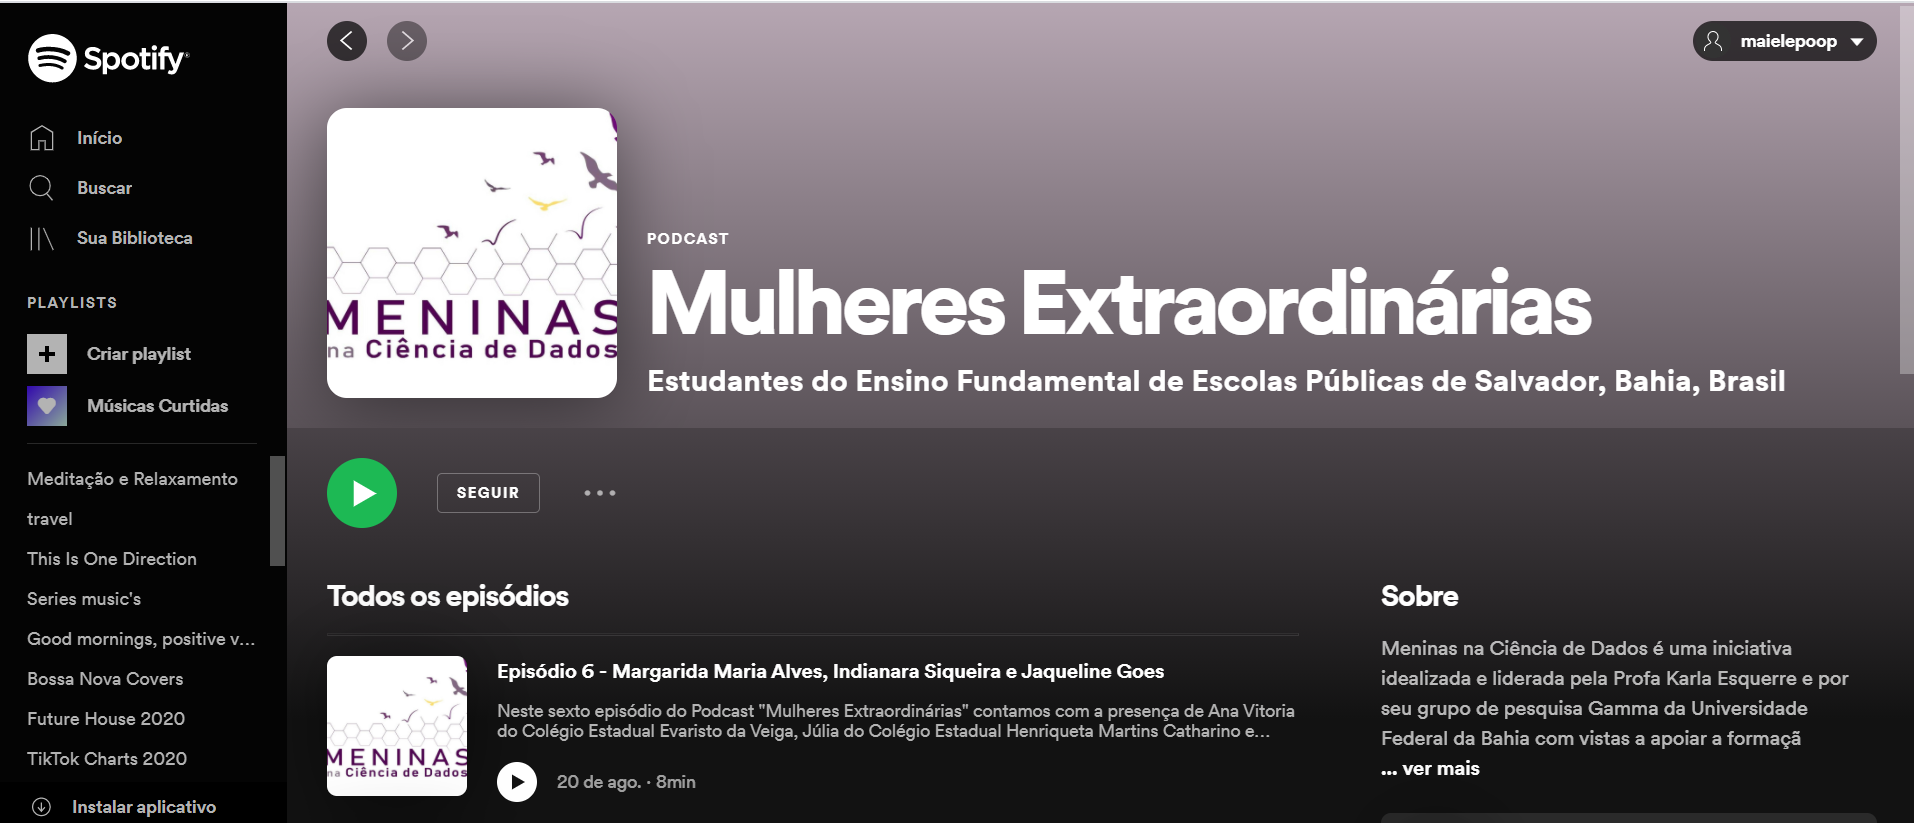
\includegraphics[width=26.58in]{images/image95} \caption{Podcast Mulheres Extraordinárias publicado pelas estudantes no Spotify. A edição dos áudios e as publicações no Spotify são de responsabilidade da estudante do 9º ano do ensino fundamental Maíra Oliveira Esquerre (voluntária).}\label{fig:podcast}
\end{figure}

\hypertarget{encantamento-do-puxfablico-escolar}{%
\section{Encantamento do público escolar}\label{encantamento-do-puxfablico-escolar}}

Uma preocupação contínua durante todo o projeto tem sido criar meios
de encantar e apoiar a formação de toda a comunidade escolar,
especialmente, estudantes, professoras/es e coordenadoras/es, das
escolas participantes do projeto, e futuramente de outras escolas.
Sendo o encantamento a etapa inicial e fundamental, uma nova
estratégia foi proposta e realizada, considerando as limitações da
pandemia. A partir da segunda semana de agosto (dia 10), visando este
público escolar das escolas participantes do projeto, a equipe do
projeto passou a compartilhar diariamente vídeos curtos (de 5 a 6
minutos de duração), disponíveis na internet e de fontes consideradas
confiáveis, relacionados aos temas explorados nos encontros com
estudantes e nos E-books em construção. Com isso, professoras/es e
coordenadoras/es das cinco escolas participantes se responsabilizaram
por compartilhar com suas/eus respectivas/os estudantes. Os vídeos
estão disponíveis no \href{https://cienciadedadosep.wixsite.com/estudantes/videos}{site do projeto} e
foram compartilhados nos grupos de WhatsApp do projeto. Na Figura
\ref{fig:exemplosvideo}
são apresentados exemplos de alguns vídeos. As estatísticas de acesso
aos vídeos não foram estimadas por falta de dados, visto que os vídeos se encontram em websites de acesso público.

\begin{figure}
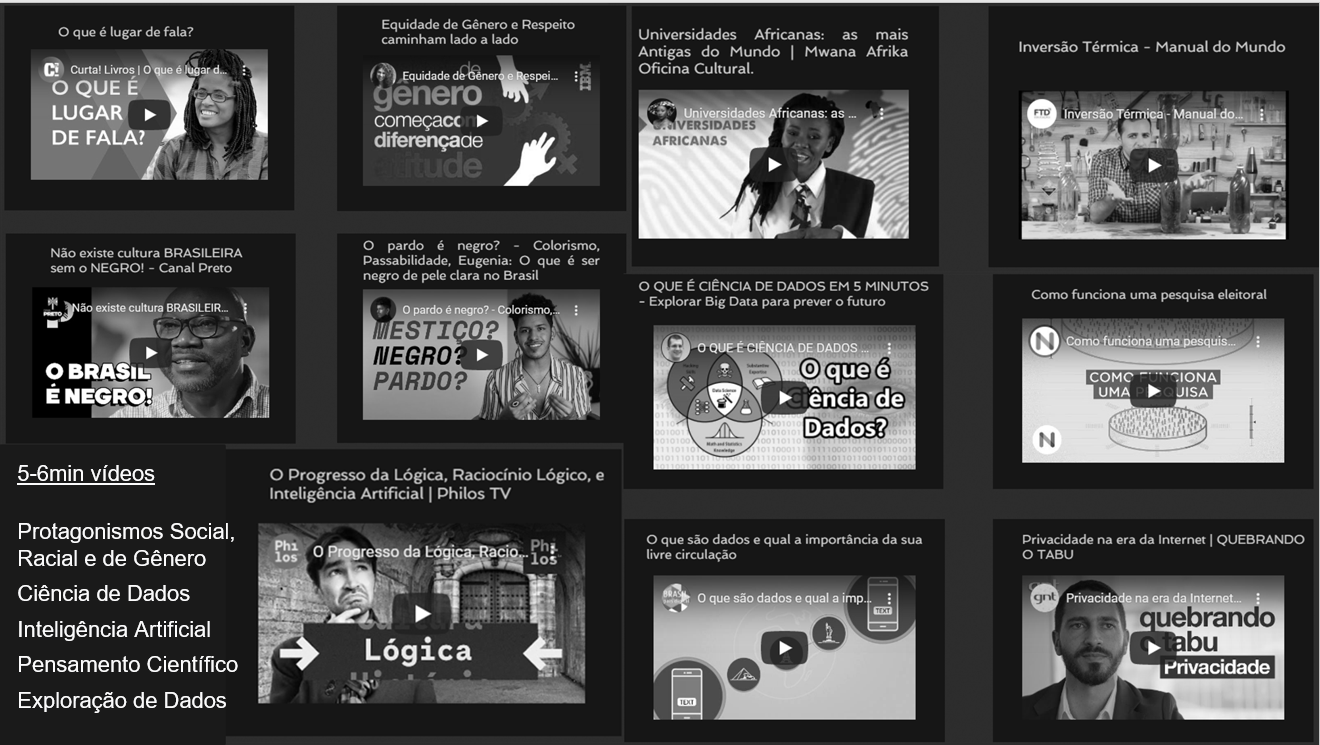
\includegraphics[width=18.33in]{images/image96} \caption{Exemplos de vídeos compartilhados com as/os estudantes e professores.}\label{fig:exemplosvideo}
\end{figure}

Visando acessar um público escolar ainda maior, além dos que fazem parte das cinco escolas que colaboram com o Projeto, a equipe colaborou de forma expressiva na Semana Nacional de Ciência e Tecnologia, promovida pela UFBA e realizada entre os dias 17 a 23 de outubro de 2020 - \href{http://www.snct.ufba.br/programacao-semana-ufba/}{(SNCT)}. Durante toda a semana, professores, estudantes e técnicos administrativos das diversas Unidades Acadêmicas da UFBA, de Salvador e Camaçari, bem como professores e estudantes da rede pública de ensino, estadual e municipal dessas cidades, participaram de encontros virtuais (palestras, mesas-redondas, bate-papos, etc) com o intuito de proporcionar discussões a respeito da Inteligência Artificial e temas afins.\\
No Quadro \ref{tab:quadro5} apresenta-se o calendário das apresentações lideradas pela equipe do Projeto, assim como o seu respectivo número de participantes. As apresentações podem ser acessadas no \href{https://www.youtube.com/playlist?list=PLdPylXX7C_XhxUyoDBxeEIOR0hbLNHbqX}{Youtube.}

\begin{table}

\caption{\label{tab:quadro5}Seminários apresentados pela equipe na Semana Nacional de Ciência e Tecnologia da UFBA 2020.}
\centering
\begin{tabular}[t]{l|l|l|l}
\hline
Data & Tema & Equipe responsável & Número de participantes total / Estudantes do projeto\\
\hline
19/10/20 10h30-11h40 & Onde está a IA no dia-a-dia: Aplicações da Inteligência Artificial & Inteligência Artificial & 60 / 14\\
\hline
19/10/20 15h-16h & O que é Inteligência Artificial e Jogos & Inteligência Artificial & 30 / 12\\
\hline
19/10/20 16h-17h & O que é Ciência de Dados? & Ciência de Dados & 26 / 11\\
\hline
20/10/20 17h-18h & Exploração Gráfica – (re)Conhecendo Salvador (Parte 1 – Mapas, população e números) & (re)Conhecendo Salvador & 24 / 10\\
\hline
20/10/20 16h-17h & Anedotas ou dados: como basear nossas conclusões? & Ciência de Dados & 23 / 10\\
\hline
20/10/20 17h-18h & Exploração Gráfica – (re)Conhecendo Salvador (Parte 2 – Gráficos e Estatísticas – Transporte, segurança e turismo) & (re)Conhecendo Salvador & 16 / 6\\
\hline
21/10/20 17h-18h & Discriminação racial algorítmica & Protagonismo & 24 / 12\\
\hline
22/10/20 14h-15:30h & Projeto Científico na Prática & Pensamento Científico & 37 / 14\\
\hline
20/10/20 & Protagonismo Feminino na Ciência de Dados & Protagonismo & 22 / 11\\
\hline
\end{tabular}
\end{table}

A Figura \ref{fig:ondeestaAI} apresenta um registro da participação da equipe nos eventos: Onde está a IA no dia-a-dia: Aplicações da Inteligência Artificial e Projeto Científico na Prática. O primeiro contou com a liderança compartilhada das professoras Érica Nascimento e Alzira Melo, dos colégios Evaristo da Veiga e Henriqueta Martins Catharino e no segundo com a participação da estudante bolsista Isabele Xavier, do Colégio Ypiranga, que apresentou um relato da sua experiência ao elaborar o seu projeto apresentado na Feira de Ciências do Agreste Pernambucano. Esses encontros oportunizaram a equipe UFBA (graduandas/os e pós-graduandas) e das escolas (professoras e estudantes) a compartilharem a fala em um evento aberto ao público, organizado pela universidade. A Figura \ref{fig:encerrSNCT}, extraída da cerimônia de encerramento, destaca-se os relatos das estudantes presentes no ambiente do chat, em que declaram os seus sentimentos em participar do Projeto, e de uma estudante no formulário de inscrições. O Projeto Meninas na Ciência de Dados é um braço forte do atual Projeto. Ressalta-se a importância da participação dos estudantes em um evento organizado pela universidade, mesmo de forma virtual, pois para a maioria o acesso à universidade ainda é muito distante.

\begin{figure}

{\centering 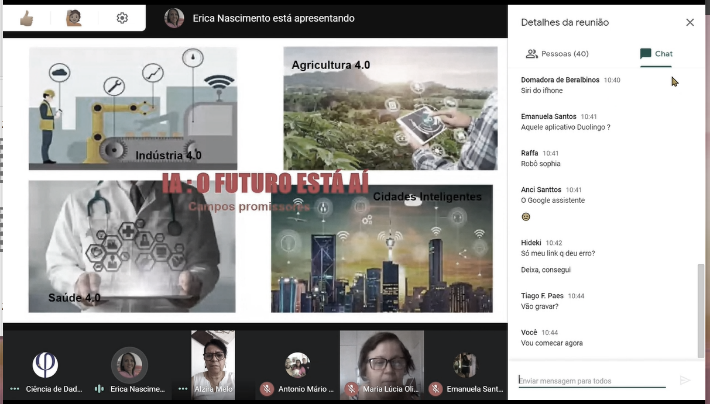
\includegraphics[width=0.49\linewidth,height=0.2\textheight]{images/image98} 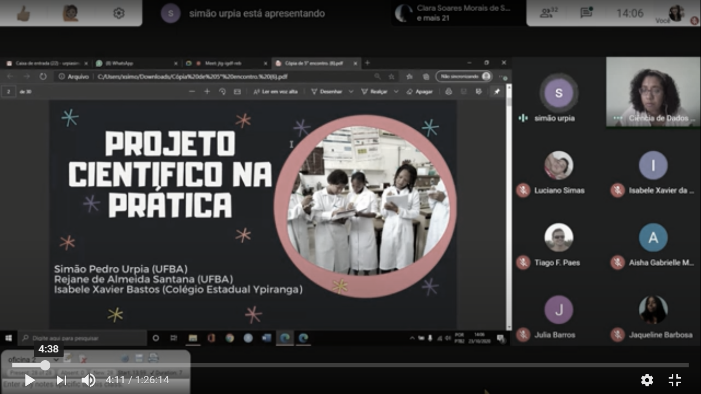
\includegraphics[width=0.49\linewidth,height=0.2\textheight]{images/image99} 

}

\caption{Registro do encontro no tema Onde está a IA no dia-a-dia: Aplicações da Inteligência Artificial, liderado pelas professoras Érica Nascimento e Alzira Melo dos Colégio Evaristo da Veiga e Henriqueta Martins Catharino, respectivamente, e pela equipe e do encontro no tema Projeto Científico na Prática, liderado pela equipe e com a participação da estudante Isabele Xavier.}\label{fig:ondeestaAI}
\end{figure}

\begin{figure}
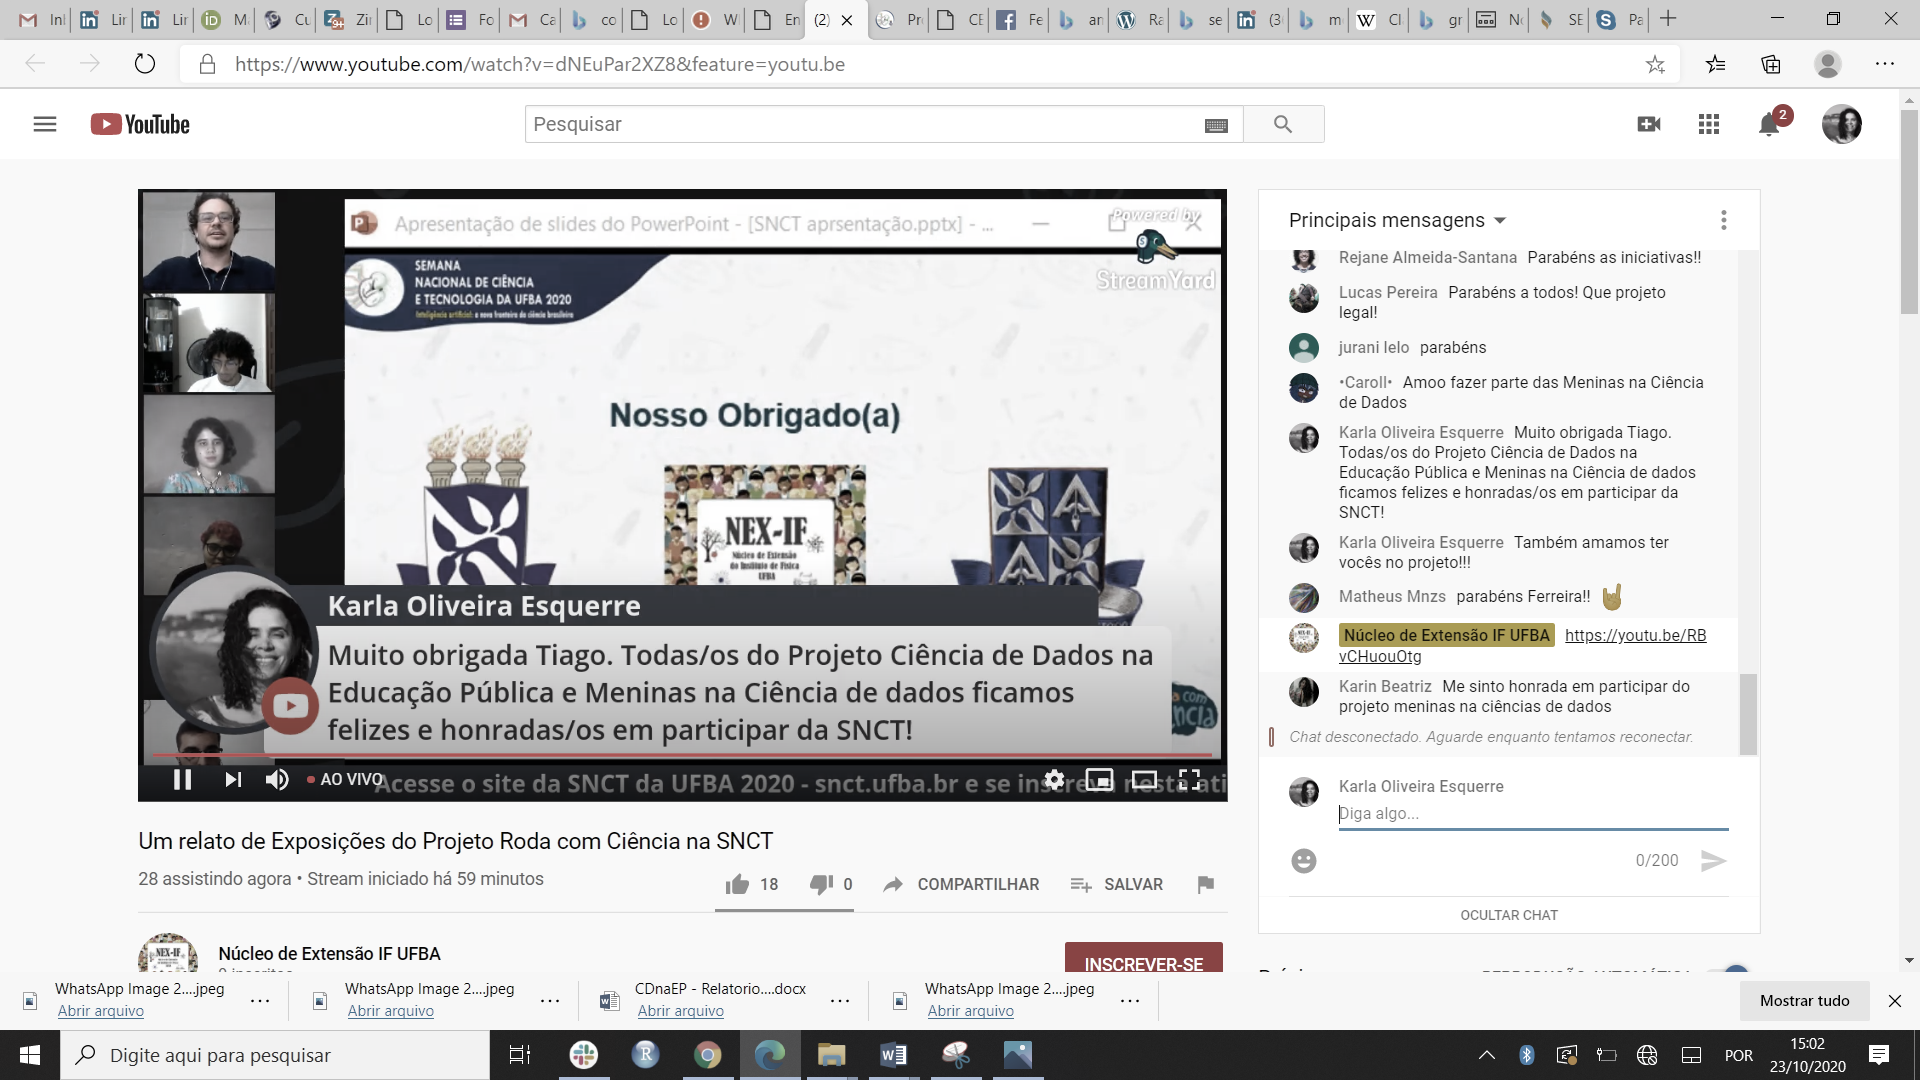
\includegraphics[width=26.67in]{images/image101} \caption{Registro da cerimônia de encerramento da SNCT. Com destaque o relato no chat das estudantes Caroll (Carollyne Dourado) “Amoo fazer parte das Meninas na Ciência de Dados” e Karin Beatriz (de Souza) “Me sinto honrada em participar do projeto meninas na ciências de dados” (esquerda) e o depoimento de um estudante no formulário de inscrições - informação compartilhada pela coordenação do evento; autoria não divulgada (direita).}\label{fig:encerrSNCT}
\end{figure}

\hypertarget{avaliauxe7uxe3o-de-impacto}{%
\chapter{Avaliação de Impacto}\label{avaliauxe7uxe3o-de-impacto}}

Tratando-se da avaliação de impactos de projetos sociais é fundamental estabelecer quais os resultados esperados, métricas e instrumentos para verificar o status deles e métodos para contornar vieses. A teoria da mudança é um método que facilita a construção de uma cadeia de elementos que parte dos insumos necessários para as atividades de um projeto e chega até os efeitos estimados no público-alvo. Métricas devem ser relevantes para o público-alvo, tão fáceis quão possível de obter e precisas no que estão medindo. Além disso, é importante ponderar que podem haver características não-observadas no público alvo e que afetam as métricas escolhidas (INSPER METRICIS, 2018).
Os principais resultados que esperamos observar como consequência das atividades que as/os estudantes participaram são:

\begin{enumerate}
\def\labelenumi{(\alph{enumi})}
\tightlist
\item
  estudantes ganham instrumentos na luta contra a desigualdade,
\item
  estudantes adquirem novas perspectivas e habilidades socioemocionais e
\item
  estudantes adquirem habilidades de letramento científico e em dados.
\end{enumerate}

\textbf{A avaliação dos impactos do Projeto está sendo construída. Neste relatório são apresentadas percepções com base qualitativa obtidas a partir dos encontros com as/os estudantes e professoras/es e dos materiais produzidos por eles. Para mensurar tais resultados foram planejadas avaliações qualitativas e quantitativas cujos resultados são apresentados no relatório anual.}
Os professores também tomaram parte em atividades no Projeto, entretanto a pandemia demandou uma mudança de planos da equipe. A intenção inicial para o ano de 2020 era maior foco no contato com os professores para que ferramentas da ciência de dados e questões sobre protagonismos social, racial e de gênero foram integradas aos conteúdos discutidos em sala de aula. Uma vez que a quarentena impediu a realização de aulas presenciais e até mesmo à distância nas escolas, a atividade liderada pelos professores não foi realizada como esperado. Não obstante, duas professoras, passaram a ministrar a disciplina de Inteligência Artificial para estudantes do ensino médio de suas respectivas escolas, e passou a ministrar palestras em eventos públicos sobre o tema. Elas têm sido exemplos de lideranças para as/os demais professoras/es.

\hypertarget{percepuxe7uxf5es-com-base-qualitativa}{%
\section{Percepções com base qualitativa}\label{percepuxe7uxf5es-com-base-qualitativa}}

\hypertarget{questuxf5es-sociais}{%
\subsection{Questões sociais}\label{questuxf5es-sociais}}

As/os estudantes demonstraram uma percepção mais aguçada em relação a questões sociais ao longo dos encontros realizados no ano. Assim, atas das reuniões semanais contendo impressões da equipe e paráfrases do que foi dito pelas/os alunas/os evidenciam essa habilidade adquirida. É importante notar que as/os estudantes desconheciam ou tinham pouca ciência acerca da atuação decisiva das mulheres em diversos campos de atuação, o que destituiu a ideia fabricada pela sociedade patriarcal que marca o local feminino em áreas estritamente ligadas ao cuidado ou ainda a concepção de mulheres como donas de casa, mães, esposas\ldots{} Por isso, ao serem apresentadas a mulheres (chamadas de extraordinárias) atuando em diversas áreas, em diferentes contextos sociais, geográficos, culturais e de época, o construto do papel da mulher na sociedade passou a ser questionado e deslocado. Foi imprescindível para garotas perceberem que elas podem assumir o papel de protagonistas nas mais diversas áreas, inclusive destituindo o que imaginavam para si, reproduzindo os papéis desenvolvidos por familiares, especialmente mães e avós, sem muitas perspectivas de subversão da realidade. É importante salientar que as garotas partícipes do projeto são de comunidades em condição de vulnerabilidade social, nas quais, as mulheres ainda são vistas sob a égide do patriarcado.\\
Em um encontro que tratou do esforço para garantir a acessibilidade a deficientes visuais, foi apresentada a educadora e ativista Dorina Norwill, as/os estudantes foram além do escopo das perguntas orientadoras. Eles pensaram a acessibilidade de uma escola para além da estrutura física e chamaram a atenção para a importância de ``que elas (deficientes visuais) socializem e não sejam excluídas e que deviam frequentar a mesma escola''. Uma das estudantes acrescentou ``que se deve evitar o bullying''.
Em outro encontro, tratando da adolescente alemã, vítima do holocausto, Anne Frank e o diário que ela escreveu relatando suas experiências em meio à guerra os estudantes foram capazes de associar as ameaças do passado com os problemas do presente. Apesar de Anne Frank ter sido uma menina perseguida na Europa devido à sua etnia e cultura judaica, as/os estudantes chamaram a atenção para pessoas podem ser perseguidas por ``seguir uma religião'', por ser homossexual ou por não gostar de uma opinião política, por exemplo.
As/os estudantes também manifestaram perceber como a representação dos negros pode reforçar estereótipos. Em um encontro (24/04) sobre Ruth de Souza, atriz negra e ativista, uma das estudantes criticou um papel que a atriz assumiu representando uma escrava. A estudante afirmou que ``papéis como esse dão a ideia de que todo negro é escravo''.
Uma estudante também demonstrou perceber de maneira intuitiva parte do conceito de interseccionalidade. Ao ser indagada sobre diferenças como o machismo incide sobre mulheres negras e brancas ela indicou que ``mulheres negras sofrem machismo e racismo ao mesmo tempo''.
Diversas estudantes relataram experiências de racismo em primeira mão, seja como vítimas ou testemunhas, adotando uma postura empática, algumas até buscaram trazer os agressores à luz do conhecimento.
O destilado dos vários aprendizados das/os estudantes foram os glossários coletivos. Esses documentos apresentam definições de palavras importantes para entender as questões sociais, raciais e de gênero. Tal documento foi uma construção coletiva baseado nas dúvidas e na pesquisa prévia realizada pelas estudantes. A elaboração foi feita em uma plataforma visível para todos. Algumas palavras definidas pelas/os estudantes foram: branquitude, matriz de dominação, representatividade e homem universal.

\hypertarget{letramento-cientuxedfico-e-em-dados}{%
\subsection{Letramento científico e em dados}\label{letramento-cientuxedfico-e-em-dados}}

Os encontros das equipes de Ciência de Dados, do Site e Produção do Conhecimento Científico foram estruturados de forma que os objetivos fossem explícitos nos relatos das equipes em ata. Esses documentos indicam que objetivos foram considerados pela equipe como alcançados com sucesso.

Em termos de letramento científico, foi relatado que as/os estudantes:

\begin{itemize}
\tightlist
\item
  Demonstraram interesse na discussão sobre onde, como e quem faz ciência;
\item
  Aqueles que tiveram experiência anterior com projetos científicos se empolgaram em compartilhar sua experiência com os colegas;
\item
  Participaram de atividades de formulação de problemas, levantamento de hipóteses de solução e estratégias para testá-las;
\item
  Discutiram métodos (entrevistas, observações, etc.) de coleta de dados e ferramentas (livros, balanças, etc.) para tal. Bem como estabeleceram um cronograma de ações.
\end{itemize}

Em termos de letramento em dados, foi relatado que as/os estudantes:

\begin{itemize}
\tightlist
\item
  Tiveram facilidade e curiosidade para identificar e analisar os elementos de mapas e gráficos apresentados sobre a cidade de Salvador;
\item
  Puderam perceber tempo, espaço e transformação de um local da cidade através da apresentação de fotos;
\item
  Interpretaram com facilidade e discutiram coletivamente elementos como o padrão de cores dos mapas, a importância da legenda, os diferentes tamanhos e cores das regiões e dos círculos nos mapas;
\item
  Confrontaram opiniões prévias que tinham quanto à proporção de estudantes matriculados do sexo feminino e masculino com dados coletados e foram capazes de incorporar as informações novas às suas noções;
\item
  Foram capazes de sugerir mudanças relevantes para aprimorar os gráficos de matrículas apresentados como: padrão das cores, escala mais exata, aumento da fonte da legenda, uso das tabelas, etc.;
\item
  Algumas/ns estudantes demonstraram interesse, discutiram e construíram análises sobre os sistemas de notificação de infrações de trânsitos de Salvador e perceberam a mudança de comportamento do número de ocorrências desses eventos por meio de gráficos (barras e boxplot), bem como os recortes temporais que os colocam frente ao momento da pandemia;
\item
  A compreensão da importância do turismo gerou curiosidade sobre estratégias de identificação de padrões como a exploração da intensidade de cores e reordenação de informações do domínio temporal de estrutura linear para o modelo de blocos periódicos. Assim, eles reconheceram os meses do ano que há mais ocupação da rede hoteleira e reconheceram a quebra de padrão como os eventos especiais como Copa do Mundo e pandemia;
\item
  Aprenderam o significado de medidas centrais (média, moda, etc.) e de dispersão (amplitude, desvio padrão, etc.) em um contexto mais próximo (idade dos colegas);
\item
  Foram expostos aos conceitos de população, amostra, intervalo de confiança, aleatoriedade e margem de erro através do tema de pesquisas eleitorais. Os conceitos de inferência estatística e intervalo de confiança foram reforçados através de uma atividade lúdica;
\item
  As manifestações de algumas/ns estudantes revelam indícios que houve o processo introdutório do letramento em dados, as perguntas geradas por informações anteriormente não citadas nos encontros, a abordagem de problemas com base em evidências são algumas das formas percebidas.
\end{itemize}

As/os estudantes também realizaram tarefas de casa que envolviam representação gráfica, cálculo de medidas e reflexão sobre dados. Elas/es passaram a reconhecer a importância das grades em um gráfico, mas mantendo uma parcimônia para não tornar a figura cheia (ver Figura 19, superior esquerda), bem como a importância da legibilidade dos eixos e a escolha de um padrão de cores para informações que correspondem a mesma categoria. Nessa atividade, surgiram diferentes métodos de representação da informação; a Figura 19 (superior direita) mostra um bom exemplo. Nessa figura também se destaca a simplicidade e elegância da representação, bem como o uso inteligente de cores no título do gráfico como maneira de comunicar facilmente o tema apresentado. Em outra atividade, as/os estudantes calcularam medidas centrais das idades de colegas. Um estudante incluiu intuitivamente em sua resolução um gráfico de pontos ou dot-plot para identificar a moda (ver Figura \ref{fig:exercestud}, inferior).

\begin{figure}
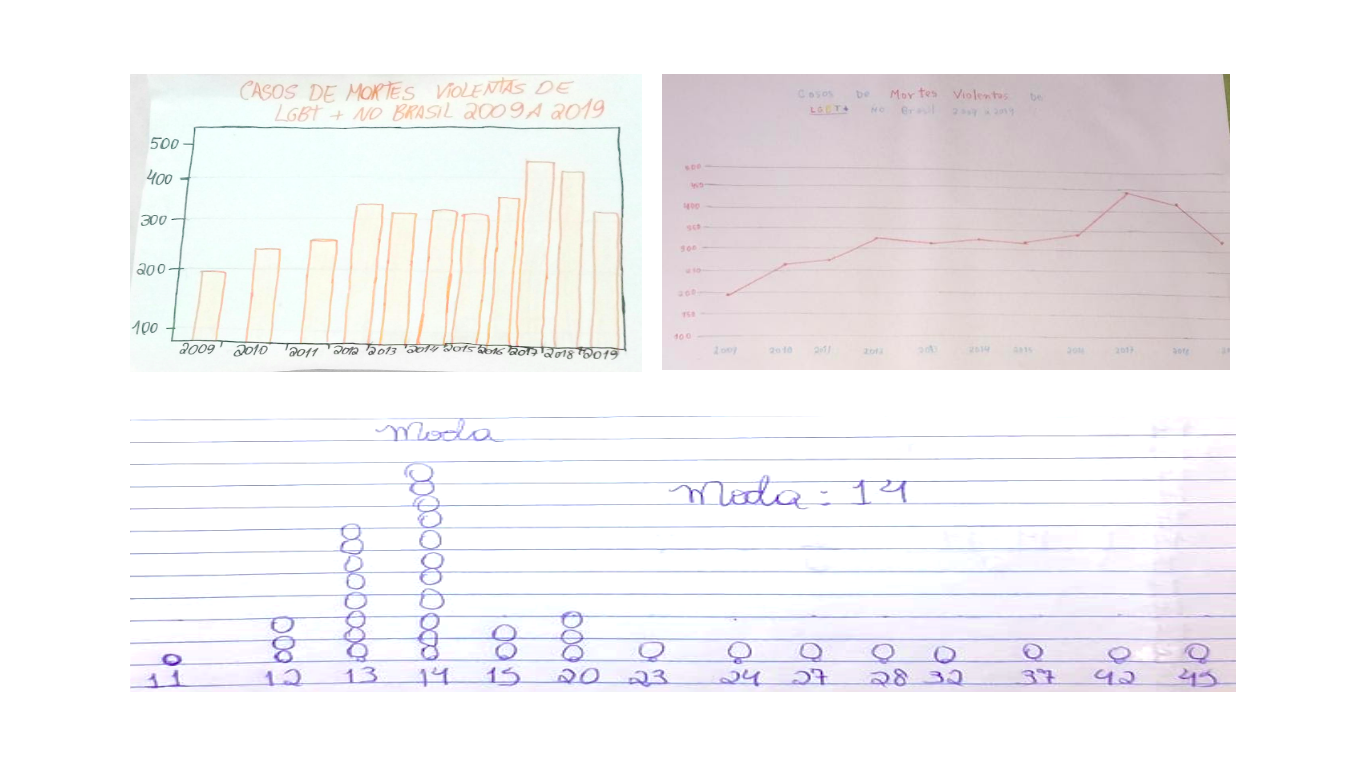
\includegraphics[width=18.97in]{images/exercico_estudantes} \caption{Gráficos produzidos pelas/os estudantes.}\label{fig:exercestud}
\end{figure}

\hypertarget{apuxeandice}{%
\chapter*{Apêndice}\label{apuxeandice}}
\addcontentsline{toc}{chapter}{Apêndice}

  \bibliography{book.bib,packages.bib}

\end{document}
